\chapter{Multi-Paradigm Integration for the \acs{BDI} Resurgence}

At the beginning of the millennium,
scenarios typical of autonomic and self-* systems
seemed to be better tackled with techniques designed for \ac{MAS},
among them, \acl{BDI} cognitive model was considered particularly promising.
%
As the years went by, however, interest decreased
in the community of self-* systems for the \ac{BDI} approach
despite new proposals still sharing a strong resemblance
with the defining features of BDI agents.
%
We argue that this trend is not a sign of the inadequacy of \ac{BDI} paradigm itself, 
rather, it is a sign of the inadequacy of the tools and frameworks available for its adoption.

% \section{Introduction}
% Computational agents are \emph{autonomous} entities~\cite{OmiciniRV08}
% situated into an \emph{environment} they can perceive and affect;
% they interact either directly or through the environment~\cite{cartago-jaamas23} by means of stigmergy.
% %
% There are several ways to model agents,
% and one of the most popular in the dedicated literature is the \ac{BDI} model.
% %

\section{An unfulfilled promise}

Since their very inception,
\ac{BDI} agents have been considered as
a promising tool for modelling autonomous or intelligent entities
via high-level \emph{cognitive} abstractions.
%
Thus,
when \ac{BDI} was turned into a programming paradigm,
at the beginning of the millennium,
the expectation of the community was for it to gain its spot among other prominent paradigms,
such as \ac{OOP} and \ac{FP},
and gain momentum specifically for systems requiring autonomy and self-management.

However,
several years later,
we observe that,
although \ac{BDI} \ac{AOP}~\cite{DBLP:journals/ai/Shoham93} had an impact on the field of \ac{MAS} and \ac{AI},
it still fails at becoming a common technique for self-* systems,
even in contexts where the dynamicity and concurrency of the application scenario would make it
a good choice to design autonomous behaviour
with high-level cognitive abstractions.

The reasons behind such a limited adoption have been openly investigated by the
\ac{BDI} programming community~\cite{DBLP:journals/sigsoft/MascardiWR19}
without reaching a consensus.
%
In 2014, Hindriks suggested to pay greater attention to the quality of the tools for engineering \acp{MAS}~\cite{DBLP:conf/dalt/Hindriks14}.
%
Four years later, the ``Agent Programming Manifesto''~\cite{DBLP:journals/ijaose/Logan18} reached apparently opposite conclusions:
although the tools are recognised as a critical factor,
the main issue seems to lie in the fact that the cost of
learning a new paradigm
is greater than implementing complex self-* behaviour in more traditional paradigms.

Indeed, in the context of autonomic computing,
extensions and modifications of the original paradigm have been proposed in the past~\cite{DBLP:conf/smc/JunJZBCJ04,DBLP:conf/prima/LiaoJG06,DBLP:journals/symmetry/KaradumanTC22},
providing evidence that, at the same time,
the paradigm can be suitable, but it may need amendments and adaptations to be effectively used in such scenarios.

\section{The road ahead}

We argue that the call for better tools
and for declinations of \ac{BDI} specific for autonomic and self-* systems are not conflicting,
rather, they are complementary:
paradigms are not immutable objects, they evolve with time and widespread use,
which cannot be attained without proper support tools.
%
Additionally,
the learning curve of a different paradigm may be reduced considerably if,
instead of a sudden mindset change,
the novel abstractions get introduced gracefully, in a way that is \emph{seamlessly integrable}
with other paradigms.

Consequently,
we believe that it is worth investigating the construction of \ac{BDI}-based toolkits
integrated into mainstream programming languages,
which could then be more easily get integrated with tools
(simulators, libraries, etc.)
used in the self-* systems community.
%
Then, feedback from the community could be used to improve the paradigm itself,
in a virtuous cycle of co-evolution between paradigm and tools.

A step in the direction of \ac{BDI} \ac{AOP} injected into mainstream programming languages is
JS-son~\cite{DBLP:conf/emas/KampikN19},
an agent programming library for JavaScript.
%
In this work,
we introduce the community to \jakta{}~\cite{BaiardiBCP23},
a further step forward in this direction,
leveraging a recent, quickly-growing, multi-paradigm language:
Kotlin,
released first in 2016,
and with a fast-growing community due to its versatility and robustness.
%
\jakta{} is an attempt to integrate the \ac{BDI} \emph{within} Kotlin
in form of an internal \ac{DSL},
thus inheriting all Kotlin-native mechanisms,
an approach successfully used by other tools used in the self-* systems community, such as Scafi~\cite{DBLP:journals/softx/CasadeiVAP22}.
%
\jakta{} is meant to improve:
%
\begin{itemize}
    \item the interoperability among \ac{BDI}/\ac{AOP} and other programming paradigms;
    \item the reuse of existing tools supporting the development of \emph{complex} \ac{BDI} codebases
    (e.g.,~\acp{IDE}, testing suites, etc.);
    \item the support for simulating and debugging \acs{BDI} agents;
    \item the concurrency and communication options.
\end{itemize}
%
\jakta{} is still in its early stages;
although experimental,
it has been open-sourced for the community to experiment with\footnote{https://github.com/jakta-bdi/jakta}.

One first step towards the integration of \jakta{} with other tools in the self-* systems community
has been its integration with the Alchemist Simulator~\cite{PianiniJOS2013},
which we used to build a drone coordination scenario as a reference scenario to understand how the \ac{BDI} paradigm
could be amended to simplify the construction of complex systems.
%
In future work,
we intend to experiment \jakta{} integration with other tools,
trying to shape its evolution based on practical use cases.

\chapter{Blending BDI Agents with \acs{OOP} and \ac{FP} with \jakta{}}
\label{chap:jakta}

This chapter focuses on the engineering choices behind embedding \ac{BDI} abstractions into mainstream languages via domain-specific languages. 
%
We define and contrast the trade-offs of \emph{internal} and \emph{external} \acp{DSL},
motivate the choice of Kotlin as a host language, 
and introduce \jakta{}, 
our Kotlin-based internal \ac{DSL} for \ac{BDI} agents.

Modern general-purpose languages increasingly support multiple paradigms, 
allowing developers to mix \ac{OOP} and \ac{FP} idioms where convenient. 
%
\ac{GPL} with flexible syntax (e.g., Scala, Groovy, Kotlin) 
also make it feasible to design expressive \emph{internal} \acp{DSL},
capturing problem-specific abstractions but still letting the user transparently fall back to the underlying
language native abstractions when needed.
%
The construction of internal \acp{DSL} plays particularly well with statically and strongly typed languages,
for which the \ac{IDE} can usually provide better contextual assistance.

Although, originally,
\acp{DSL} were meant to provide dedicated abstractions for specific domains,
there is no principled reason for them not to be used to model a full-fledged paradigm.
%
Arguably,
one reason discouraging such practice in most cases relates to the final ergonomics of the resulting \ac{DSL}:
since the \ac{DSL} is built on top of the host language,
it is bound to the syntactic constraints of the latter,
which may end up hindering the expressiveness of the \ac{DSL} too much compared to a dedicated language.

Oppositely,
most AOP languages are implemented as \emph{external} \acp{DSL},
-- commonly on top of some \ac{GPL} such as Java or Python --,
typically featuring the possibility to call the underlying \ac{GPL} code
via a \ac{FFI},
a dedicated mechanism allowing calls to code written in a different language.
%
Arguably,
the interaction between an external \ac{DSL}
and its host language through a \ac{FFI} is not as seamless as the one between an internal \ac{DSL} and its host language,
as GPL code is isolated from the \ac{DSL},
and ad-hoc syntactical features are required to ``call'' it from the \ac{DSL}.
%
Furthermore,
an external \ac{DSL} requires users (resp. developers),
to spend additional effort in learning (resp. realising and maintaining)
both a new language (parser) and
an ecosystem of tools
(e.g., debugger, syntax coloring, linter, \acp{IDE}, etc.).

To the best of our knowledge,
no mainstream programming language prior to this work 
\emph{natively} supports the \ac{AOP} paradigm,
especially the \ac{BDI} model.
%
The current state of the art includes several stand-alone programming languages
that support \ac{BDI} agents programming following the well-known
\agentspeak{}~\cite{rao1991bdi} semantics---such as
\jason~\cite{BordiniHW2007}, \astra~\cite{CollierRL15}, and \goal~\cite{Hindriks2009}.
%
However,
using and maintaining stand-alone languages can be burdening,
especially when the community of contributors is small, since
languages usually require several tools to be usable in practice
(e.g., content assistants, syntax highlighters, linters, debuggers, etc.)
whose development and maintenance adds upon the cost of the language itself---%
potentially causing the ecosystem to evolve slowly,
thus hindering adoption.

This chapter presents \jakta{}, 
a Kotlin internal \ac{DSL} that aims to combine the expressiveness of \ac{BDI} abstractions 
with the practical benefits of a mainstream host language. 
%
The objectives motivating this design are:
\begin{inlinelist}
    \item preserve a familiar \ac{BDI}-style programming model for practitioners, 
    while making it idiomatic to Kotlin developers;
    \item reuse existing tooling and libraries to lower the adoption and maintenance costs of the language; and
    \item enable interoperability between \ac{BDI} code and ordinary \ac{OOP}/\ac{FP} code, 
    supporting multi-paradigm systems and easier integration with simulators and other tooling.
\end{inlinelist}

We introduce \jakta{} as an implementation that demonstrates these trade-offs. 
%
The \ac{DSL} is implemented as a Kotlin library and reuses its language features
(type-safe builders, lambdas with receiver, extension functions) 
to provide a compact, 
type-checked syntax for declaring 
agents, 
beliefs, 
plans, 
and environments.
% 
Where appropriate, 
the chapter highlights practical benefits such as \ac{IDE} support, 
code reuse, and safer composition with Kotlin code.

The remainder of the chapter describes the \ac{DSL} design and the interpreter architecture (Section~\ref{sec:jaktadsl}), illustrates the approach via examples (Section~\ref{sec:running-example}), and discusses limitations and future directions (Section~\ref{sec:conclusion}).

\section{Background}
\label{sec:background}

This work lays on two pillars: \ac{DSL} engineering (specifically, internal Kotlin \acp{DSL}) and \ac{BDI} agents programming.
%
In this section,
we briefly introduce them by discussing the principles behind the creation of \acp{DSL}
and we explain how and why modern languages support the creation of \textit{internal} \acp{DSL}.
%
We also provide a comparison among a selection of existing \ac{BDI} programming frameworks from the literature,
discussing how syntactical aspects may impact their interoperability and versatility.
% \sbsidenote{ho aggiunto due frasi solo perché non mi piaceva restare estremamente scarno, liberi di tagliare di nuovo se non vi piace}

\subsection{\ac{DSL} engineering}
\label{subsec:internal-vs.-external-domain-specific-languages}
\acp{DSL} are programming languages tailored to specific domains:
they expose the domain model entities and their interactions as first-level abstractions.
%
However, there is no rule on which amount of domain-specificity makes a language a \ac{DSL}:
at some level, every language is domain-specific,
with the specific domain being the \emph{paradigm} the language is rooted in.
%
For instance,
we argue that even the \ac{ASL}
can be seen
as a \ac{DSL} modelling the domain of \ac{BDI} agents.

From a technical perspective,
\acp{DSL} can be classified into two broad categories~\cite{Riti2018}:
\emph{external}, if they are stand-alone, with their own custom syntax and compiler/interpreter;
and \emph{internal}, if they are embedded in a host language and rely on the syntactic and semantic features of the host.
%
From the point of view of the host language,
internal \acp{DSL} are indistinguishable from ordinary libraries
(indeed, as C++ inventor Bjarne Stroustrup used to say, ``library design is language design''~\cite{Stroustrup1997}),
their distinction is usually driven by their \emph{purpose}\footnote{
    \href{https://archive.is/xAeiX}{Martin Fowler's blog post on DSL Boundary archived at https://archive.is/xAeiX}
}.
%
Consequently,
internal \acp{DSL} might \emph{in principle} be realised in any language;
\emph{in practice}, however,
the host language syntactic flexibility directly reflects on the ergonomics of any internal \ac{DSL}.
For this reason,
several recent languages (e.g., Scala, Kotlin, Ruby, Groovy)
provide syntactic features specifically tailored to the constructions of internal \acp{DSL}.
%
Although these features make internal \acp{DSL} viable,
they can hardly provide an expressiveness comparable to that of an external \ac{DSL},
as they are still bound to the host language syntax.

A notable example of a feature designed for \ac{DSL} engineering which is at the same time an enabler and a limit
is the lambda expression syntax of Kotlin and Groovy.
%
In both languages, the following evaluates to an anonymous function:
\lstinline[language=Kotlin,breaklines=false]|{ arguments -> body }|%
,
which can be further simplified to
\lstinline[language=Kotlin,breaklines=false]|{ body }|
for 0-ary lambdas or 1-ary lambdas using
\lstinline[language=Kotlin,breaklines=false]|it|
as implicit name for the single argument.
%
This peculiar syntax is designed to be used effectively in conjunction with the \emph{trailing lambda convention},
by which any function accepting a lambda expression as its last argument can be invoked by moving the lambda expression outside the round parentheses;
additionally, if the lambda expression is the only argument, the round parentheses can be omitted altogether.
%
For instance, a function with signature
\lstinline[language=Kotlin,breaklines=false]|fun myBlock(body: () -> Any)|
taking a single 0-ary lambda expression as its argument can be invoked as
\lstinline[language=Kotlin,breaklines=false]|myBlock{"I love DSLs"}|%
,
providing the feeling of a custom block of code named as the higher-order function
\lstinline[language=Kotlin,breaklines=false]|myBlock|%
.
%
Although this feature makes the construction of new \ac{DSL} blocks particularly easy,
the price to pay is that most \ac{DSL} constructs must be enclosed in curly braces,
thus limiting the \ac{DSL} design freedom.

Selecting whether an internal or external \ac{DSL} is best for the problem at hand is a matter of trade-offs:
as discussed, internal \acp{DSL} have limited syntactic flexibility that could result in a less expressive language,
but, in turn, they inherit from their host:
\begin{inlinelist}
    \item the tooling
        (IDE support, build systems, linters, debuggers, profilers, and so on),
        reducing the maintenance burden;
    \item the libraries,
        reducing the need for ad-hoc solutions; and
    \item the abstractions,
        allowing the \ac{DSL} to be used in conjunction with other paradigms.
\end{inlinelist}
%
Together, these aspects may also lower the learning curve for those already acquainted with the host language,
possibly favouring wider adoption.

In fact,
besides the language ergonomics itself,
the success of a language is also determined by the availability of a rich ecosystem of libraries and tools
(syntax highlighting, code completion, live error detection, assisted refactoring, debuggers, linters, profilers, etc.),
lowering the learning curve and supporting advanced practical uses.
%
Here lies a key motivation for favouring internal \acp{DSL} over external ones:
most (often, all) of the pre-existing tooling for the host language can be reused for the new internal \ac{DSL},
reducing \emph{both} maintenance costs and learning curve.
%
From the point of view of developers and maintainers,
time and resources that would have been spent into developing and maintaining part of the tooling and documentation can be redirected to other improvements;
from the point of view of users,
pre-existing knowledge of the host \ac{GPL} language and its tooling can be leveraged to quickly start with the new \ac{DSL},
and, for the newcomers, most of the documentation and tutorials for the host language can be reused.

\subsection{Kotlin as a Host Language for Internal \acp{DSL}}
\label{sec:dsl}

Internal \ac{DSL}-like solutions may be realised in virtually any GPL, for instance by defining a \emph{fluent} \ac{API}~\cite{Riti2018}.
%
In that case, users would write their \ac{DSL} code by chaining method calls, while still using ordinary \ac{OOP} constructs.
%
However, recent languages such as Scala, Kotlin, or Ruby come with a flexible syntax which gives \ac{DSL} designers great flexibility in extending the hosting GPL with new constructs.

In the particular case of Kotlin as the hosting \ac{GPL},
internal \ac{DSL} design leverages primarily the following set of features%
\footnote{
    A comprehensive review of Kotlin's features that can be exploited for building \acp{DSL}
    is beyond the scope of this chapter,
    but we refer the interested reader to the Kotlin documentation about the so-called ``type-safe builders'',
    archived at \url{https://archive.is/El3fE}.
}~\cite{kotlindsi4prolog-woa2020}:
%
\begin{description}
    \item[Operator overloading\footnotemark] ---
        allowing ordinary arithmetic, comparison, access, assignment, and function invocation operators to change their ordinary meaning on a per-type basis;
        \footnotetext{Kotlin Operator overloading documentation, archived at \url{https://archive.is/m36Pl}}
    \item[Block-like lambda expressions and trailing lambda convention\footnotemark] ---
        see \Cref{subsec:internal-vs.-external-domain-specific-languages}
        \footnotetext{\label{itm:lambda}Kotlin Higher-order functions and lambdas documentation, archived at \url{https://archive.is/ym8Gf}}
    \item[Extension methods\footnotemark] ---
        allowing pre-existing types to be extended with new instance methods whose visibility is scope-sensible.
        \footnotetext{Kotlin Extensions documentation, archived at \url{https://archive.is/G9DDM}}
    \item[Function types/literals with receiver\footnoteref{itm:lambda}] ---
        allowing functions and methods to accept lambda expressions within which the \kotlinInline{this} variable references a different object than the outer scope;
\end{description}
%
Crucially for our purpose,
Kotlin-based \acp{DSL} inherit all the host language's features and libraries.
%
%Furthermore, if properly engineered, these \acp{DSL} may be executed on all the platforms supported by Kotlin%
%---which include the \ac{JVM}, JavaScript, Android, and native code for the most common platforms.
%
% This is for instance the case of our \ac{DSL} proposed in \cref{sec:contribution}.

%%HERE

\section{A Kotlin \ac{DSL} for BDI Agents}
\label{sec:jaktadsl}

We identify the core features that we need into an
implementation of a \ac{DSL} for \ac{BDI} agents familiar to \ac{BDI} experts
and idiomatic to the community of mainstream developers.
%
Thus, as first step,
we want it to be \agentspeak{}-compliant
and, at the same time,
based on a mainstream language, hence, an \emph{internal} \ac{DSL}.

Then, the language should be statically and strongly typed,
possibly featuring type inference to reduce ceremonial code.
%
Among the other features,
we considered the target platform and its portability across multiple platforms
(as we wanted to maximise the range of potential target runtimes),
the existing ecosystem (as we wanted to leverage existing libraries and tools),
the language's popularity (as we want to let the agent-orientation be available to the widest possible audience),
and the specific language features that could be leveraged for the construction of a \ac{DSL}.

We considered several languages, including Java, Scala, Kotlin, Python, Ruby, C\#, and Typescript.
%
From the point of view of syntactic flexibility we favoured Scala, Kotlin, and Ruby,
as they provide machinery specifically meant to allow the construction of \acp{DSL}.
%
We then discarded Ruby, as we wanted a statically typed language.
%
We picked Kotlin over Scala despite the latter having a richer type system
(supporting, for instance, path-dependent and higher-kinded types~\cite{JohannP19})
for merely practical reasons:
%
\begin{enumerate}
    \item Scala 3 recently broke retro-compatibility with Scala 2,
    and, at the time this work was realised,
    many libraries and tools were not yet available for the new version;

    \item we expect Kotlin's popularity to grow faster than Scala's in the future,
    as Google picked Kotlin as reference language for the Android ecosystem\footnote{
        Android’s Kotlin-first approach, archived at \url{https://archive.is/C8aR8}
    }, and

    \item Kotlin has better support for multi-targeting
    (\ac{JVM}, JavaScript, and native code including Apple-specific platforms).
\end{enumerate}

The framework has been released under a permissive \ac{FOSS} licence.
%
It is available on GitHub\footnote{
    \url{https://github.com/jakta-bdi/jakta}
} and Maven Central\footnote{
    \url{https://search.maven.org/artifact/it.unibo.jakta/jakta-dsl}
};
to ensure future references and reproducibility,
every new release is also archived on Zenodo~\cite{BaiardiCP23}.

\subsection{Overview of \jakta{}'s syntax}
\label{subsec:language-description}

In this subsection we provide an overview of \jakta{} from a syntactical perspective.
%
Details about \jakta{}'s architecture and implementation giving semantics to the syntax are left to \Cref{sec:implementation}.

The \jakta{}'s \ac{DSL} syntax is strongly inspired by Jason and it is \agentspeak{}-compliant.
%
We will not cover all details of the syntax and semantics of \agentspeak{} here,
the interested reader may refer to~\cite{BordiniHW2007}.

%At the technical level, \jakta{} source files are in fact Kotlin source files.
%%
%These could, in turn, consist of self-contained Kotlin scripts, or be part of a larger Kotlin projects.
%%
%In the following, we focus on \jakta{} compliant snippets describing \ac{MAS} specifications.

\paragraph{Program entrypoint}

The entrypoint of a \ac{MAS} specification is the \kotlinInline{mas} block,
inside whose scope all the elements composing a \ac{BDI} \ac{MAS} can be defined:
%
\lstinputlisting[
    basicstyle=\footnotesize\ttfamily,
    linewidth=\linewidth,
    language=Kotlin,
]{listings/sncs24/jakta-examples/mas_dsl.kt}
%
Commonly, users configure the environment, and provide initial agents' specifications within this block.
%
Intuitively, The environment is configured in the \kotlinInline{environment} block,
and it may impact all agents
in the \ac{MAS}.
%
Single agent specifications are provided by means of the \kotlinInline{agent} block,
specifying the agent's name.

From this first snippet,
it is evident how the Kotlin syntactic features are being leveraged to build the \ac{DSL}.
%
More specifically, both \kotlinInline{mas} and \kotlinInline{environment} are a 1-ary functions taking,
as a single parameter,
a function (with receiver), which in this example is provided as a lambda expression
(notice the curly braces syntax);
since it is the sole parameter, the round braces of function invocation can be omitted altogether
as per the trailing lambda convention.
%
Similarly, \kotlinInline{agent} is a binary function function taking a \kotlinInline{String} as first parameter
and a function (with receiver) as the second parameter.
%
In this case, the round braces of function invocation cannot be omitted,
yet the lambda expression can be passed outside them
(again, trailing lambda convention),
providing the feeling of a custom keyword and related code block.
%
Through this kind of mechanism,
\jakta{} injects \ac{AOP} in the form of perfectly legitimate Kotlin code.

Finally, the snippet shows how the \ac{MAS} can be directly executed, by invoking the \kotlinInline{start} method.
%
As \jakta{} is an internal \ac{DSL}, the whole specification is done through valid Kotlin code.
%
We can though distinguish two phases:
\begin{inlinelist}
    \item first, the Kotlin code within the \kotlinInline{mas} block is executed
        assembling the structure of the \ac{MAS} from its declarative definition
    \item then, when the \kotlinInline{start} method is invoked, the MAS is executed by the BDI interpreter described in \Cref{sec:implementation}.
\end{inlinelist}.
%
%The execution and the \ac{MAS} definition can also happen in two different times:
%the programmer can firstly define the \ac{MAS} specification and then, successively, execute it.
%\mbsidenote{Per samubura, ti piace?}

\paragraph{Agents}

Agents are named entities created with the \kotlinInline{agent} function. %\sbsidenote{keyword?}
%
Inside the \kotlinInline{agent} block
(the lambda expression passed as last parameter)
\kotlinInline{beliefs}, \kotlinInline{goals}, internal \kotlinInline{actions} and \kotlinInline{plans},
can be defined in homonym blocks.

These few syntactic elements are enough to show a hint of how blending paradigms can be leveraged to build complex systems in a few lines of code.
%
In the following example, we mix \ac{OOP}, \ac{FP}, and \ac{AOP}:
we fetch the athletes' names from a public web page indexing Olympic athletes,
we extract ten names through a regular expression,
and then we create one agent for each athlete:
\lstinputlisting[
    linewidth=\textwidth,
    language=Kotlin,
]{listings/sncs24/jakta-examples/blending.kt}
%
In this example, we exploit \jakta{} for the \ac{MAS} definition,
the \ac{OOP} paradigm to deal with the regular expression match and data extraction from the group,
and the functional paradigm to monadically map web URLs to athletes.

\paragraph{Beliefs}

Beliefs are represented as a logic theory,
namely, a collection of \emph{facts} and \emph{rules} expressed in a logic programming fashion.
%
\jakta{} directly leverages (and exposes as an \ac{API})
the logic programming toolkit for Kotlin \twopkt{}~\cite{2pkt-swx16} and its internal \ac{DSL} for Prolog~\cite{kotlindsi4prolog-woa2020}.

For instance,
in the following, we define a belief base containing information about paths in a graph,
by means of logic facts, as well as logic rules for computing whether some location
\prologInline{X} is reachable from another location \prologInline{Y}:
%
\lstinputlisting[
    basicstyle=\footnotesize\ttfamily,
    linewidth=\textwidth,
    language=Kotlin,
]{listings/sncs24/jakta-examples/beliefs_dsl.kt}

Under the assumption that the graph represents some sort of map from the real world,
the above belief base can be exploited by the agent to reason about reachability among
any two locations in the map;
in fact, through \twopkt{},
\jakta{} fully supports Prolog's unification and resolution mechanisms.

\paragraph{Goals}

Goals can indicate either something that the agent wants to
\kotlinInline{achieve}
by finding an appropriate plan,
or something that it wants to \kotlinInline{test} (discover),
prioritising the consultation of the knowledge base over the execution of plans.

Similarly to \jason{},
\jakta{} supports the definition of agents' \emph{initial} goals
(further goals may arise during the execution of the \ac{MAS})
by means of the \kotlinInline{goals} block:
%
\lstinputlisting[
    basicstyle=\footnotesize\ttfamily,
    linewidth=\textwidth,
    language=Kotlin,
]{listings/sncs24/jakta-examples/goals_dsl.kt}
%
%As discussed in the next paragraph, the syntax of goals in plans' heads is exactly the same.

\paragraph{Plans}

Plans describe which operations the agent is capable to perform to reach its goals.
%
Inheriting the successful model of \jason{},
in \jakta{}, plans are composed of
a \textbf{triggering event} deciding whether the plan is \emph{relevant},
an optional \textbf{context} restricting its \emph{applicability},
and a \textbf{body} listing the operations to be performed whenever the plan is executed.

The triggering event can be
a goal/belief invocation/addition (\kotlinInline{+}) or failure/deletion (\kotlinInline{-}),
in the form:
{\texttt{[+|-]~<triggering~event>~onlyIf~\{<context>\}~then~\{<body>\}}}.
%
We inherit from \jason{} the usage of a prefix unary \kotlinInline{+} to indicate invocation or additions,
and a prefix unary \kotlinInline{-} to indicate failures or deletions.

If a logical expression is present in the context block (prefixed by \kotlinInline{onlyIf}),
it is then used to vet the relevant plan.
%
The condition therein expressed should be a logic formula to be tested against the belief base
via logic resolution.

Finally, if the plan is selected for execution,
the sequence of operations and actions contained in its body
(prefixed by \kotlinInline{then}) is performed by the agent.
%
There, actions may consist of edits (additions or deletions) to the belief base,
as well as additions of further achievement or test goals,
or invocations of external or internal actions (see next paragraphs).
%
\lstinputlisting[
    basicstyle=\footnotesize\ttfamily,
    linewidth=\textwidth,
    language=Kotlin,
]{listings/sncs24/jakta-examples/plans.kt}
%

\paragraph{Internal Actions}

Actions are (usually imperative) operations
that agents may invoke within plans.
%
They are meant to be used when some computation
can not be encoded conveniently in a declarative way.
%
They may also be used to get ``under the hood''
and inspect or modify the \ac{MAS} internals.

In particular, \emph{internal} actions
come with an ad-hoc \acp{API} for inspecting or modifying the agent's state,
whereas external actions provide \acp{API} for inspecting or modifying the environment.

\jakta{} provides an ad-hoc syntax for defining and invoking internal actions.

Definitions occur within an agent's \kotlinInline{actions} block,
requiring name, arity, and body
(the latter, as usual, in form of a lambda expression).
%
Inside the body,
the programmer can call
Kotlin \acp{API} dedicated to access and modify the agent's state,
and to manipulate \ac{BDI} data structures (beliefs, goals, plans, intentions).

Actions execution may occur within plans' bodies, by means of the \kotlinInline{execute} function.
%
This function takes as input the name of the action to be executed and (if any) the actual arguments to be passed.
%
The same syntax is used to invoke \emph{external} actions.

The main difference between internal and external actions is that
the former are agent-specific,
while the latter are shared.
%
In practice, this means that
each agent may only invoke internal actions defined within its \kotlinInline{actions} block,
whereas it may invoke any external action defined in the environment.

In the following snippet, we exemplify the general syntax for defining internal actions,
and the operations therein supported for agents' state manipulation.
%
Since this snippet is meant to be a general example,
we the syntax \meta{} to enclose placeholders for actual code.
%
We will use such syntax also in other snippets that follow this one.
%
\lstinputlisting[
    basicstyle=\footnotesize\ttfamily,
    linewidth=\textwidth,
    language=Kotlin,
]{listings/sncs24/jakta-examples/internal_action_dsl.kt}
%
More precisely,
internal actions provide primitives that can change the overall agent's state, not limited to its belief base, by:
\begin{inlinelist}
    \item add/remove intentions,
    \item add/remove events, that will become new agent's goals,
    \item add/remove plans,
    and
    \item pause or stop the agent.
\end{inlinelist}

Conversely, in the following snippet we exemplify the general syntax for invoking actions:
%
\lstinputlisting[
    basicstyle=\footnotesize\ttfamily,
    linewidth=\textwidth,
    language=Kotlin,
]{listings/sncs24/jakta-examples/internal_action_dsl_inv.kt}

Internal actions in \jakta{} are used frequently,
thus,
it is common for developers to share them across multiple agents,
or even across agents of different projects,
building libraries of actions.
%
Although Kotlin provides multiple means that favour reuse,
the way we recommend as \jakta{} developers is to create a Kotlin \kotlinInline{object}
(a singleton object under the \ac{OOP} abstraction)
implementing the \kotlinInline{InternalAction} \kotlinInline{interface}
and possibly extending the \kotlinInline{AbstractInternalAction} \kotlinInline{abstract class}.
%
Such \kotlinInline{object} would provide a reusable internal action,
which, as any other Kotlin \kotlinInline{object}, can be shared across agents,
shipped within libraries, and imported in other projects.
%
For instance, the \kotlinInline{Print} internal action, shown below, lets agents log on the console:
%
\lstinputlisting[
    basicstyle=\footnotesize\ttfamily,
    linewidth=\textwidth,
    language=Kotlin,
]{listings/sncs24/jakta-examples/print.kt}
%
Internal actions defined in this way can be imported in one agent's \kotlinInline{actions} block,
similarly to actions defined on the fly, and invoked
%as any other action:
%%
%\lstinputlisting[
%    basicstyle=\footnotesize\ttfamily,
%    linewidth=\textwidth,
%    language=Kotlin,
%]{listings/jakta-examples/print-usage1.kt}
%%
%However, to simplify the notation invocation-side, \jakta{} supports
%executing internal actions
by means of the corresponding Kotlin object's name:
%
\lstinputlisting[
    basicstyle=\footnotesize\ttfamily,
    linewidth=\textwidth,
    language=Kotlin,
]{listings/sncs24/jakta-examples/print-usage2.kt}

To support the most common use cases,
\jakta{} comes with several ready-to-use internal actions out of the box.
%
\kotlinInline{Print}, exemplified above, is one of them,
additional ones include
\kotlinInline{Fail}, forcibly failing the current plan;
\kotlinInline{Stop}, forcibly terminating the current agent's lifecycle;
\kotlinInline{Pause}, pausing the execution of the agent indefinitely;
and \kotlinInline{Sleep}, pausing the execution of the agent for an amount of milliseconds.

\paragraph{Environment}

Environments are first-class citizens in \jakta{}.
%
Each \ac{MAS} must have one environment, which can be configured once for the whole \ac{MAS},
by means of the \kotlinInline{environment} function.
%
Technically speaking, a \ac{MAS} environment is an instance of a class implementing the \kotlinInline{Environment} interface.
%
All agents in the \ac{MAS} have access to the environment,
which decides what agents can perceive,
how they may act,
and how agent-to-agent messages are delivered.
%
Environments may also store custom data
(in the form of key-value pairs),
which may be made visible to (or modifiable by) agents
by means of ad-hoc external actions.
%
In the \kotlinInline{environment} configuration block,
users may define or reference the \emph{external} actions that \emph{all} agents may use,
or reference a custom implementation of the \kotlinInline{Environment} interface.

The following snippet exemplifies the environment configuration.
%
\lstinputlisting[
    basicstyle=\footnotesize\ttfamily,
    linewidth=\textwidth,
    language=Kotlin,
]{listings/sncs24/jakta-examples/env.kt}
%
Custom implementations of \kotlinInline{Environment} may be used if passed to the
\kotlinInline{from} function.
%
To simplify the construction of custom environments,
we provide in the \jakta{} \ac{API} an \kotlinInline{AbstractEnvironment} \kotlinInline{abstract class};
also in \Cref{sec:running-example} we provide examples of custom environments.
%
When omitted, the system falls back to the default implementation,
working well in the majority of the cases.
%
The \kotlinInline{actions} function, in this context, is used to define or reference external actions.
%
The \kotlinInline{data} property is used to define custom data that may be accessed by agents
(either for reading or writing) by means of perception or external actions.
%
Finally, the \kotlinInline{perception} block may be used to define which percepts
shall pop up in the agent's belief bases at runtime.
%
Of course, these percepts may read any information stored into the aforementioned
\kotlinInline{data} property.

\paragraph{External actions}

External actions are the \emph{only} way for the agents to affect the environment
or to communicate with other agents.
%
Their design is akin to internal actions,
despite the fact that they come with different capabilities, and therefore a different \ac{API}
that can be exploited to
\begin{inlinelist}
    \item add/remove agents,
    \item send/broadcast messages,
    or
    \item add/remove/update data in the environment.
\end{inlinelist}
as shown in the following snippet:
\lstinputlisting[
    basicstyle=\footnotesize\ttfamily,
    linewidth=\textwidth,
    language=Kotlin,
]{listings/sncs24/jakta-examples/external_action_dsl.kt}
%
As for internal actions,
external actions can be defined in Kotlin by implementing the \kotlinInline{ExternalAction} interface,
typically using \kotlinInline{object}s,
and possibly extending the \kotlinInline{AbstractExternalAction} \kotlinInline{abstract class}.
%
For instance, the \kotlinInline{Send} external action, shown below, sends messages to other agents, given their name:
%
\lstinputlisting[
    basicstyle=\footnotesize\ttfamily,
    linewidth=\textwidth,
    language=Kotlin,
]{listings/sncs24/jakta-examples/send.kt}
%
External actions defined in this way can be imported in environments' \kotlinInline{actions} blocks,
similarly to actions defined on the fly, and invoked as any other action by agents:
%
\lstinputlisting[
    basicstyle=\footnotesize\ttfamily,
    linewidth=\textwidth,
    language=Kotlin,
]{listings/sncs24/jakta-examples/send-usage.kt}
%
%However, to simplify the notation on the invocation side, \jakta{} also supports
%executing external actions too by means of the corresponding Kotlin object's name.

\paragraph{Message-passing}

In \jakta{}, messages are exchanged through the environment,
message passing capabilities are modelled as external actions.
%
Thus, \jakta{} requires all environment implementations to handle
agents' inboxes and dispatch messages,
which enables customisation of message-passing protocols
(including distributed ones)
through the construction of personalised environments.
%
%In other words, what actually happens when an agent sends a message to another agent
%is that the environment takes the message in charge, identifies the recipient,
%and puts the message in the recipient's inbox.
%%
%This behaviour may be customised by developers of custom environments,
%for instance to support different low-level message-passing protocols.

%Regardless of the low-level technicalities,
%however,
Technically, all environment implementations must support the following functionalities:
%
\begin{enumerate}
    \item \kotlinInline{sendMessage}, which delivers a message to a specific recipient agent,
    and
    \item \kotlinInline{broadcastMessage}, which delivers the message to all agents in the \ac{MAS}.
\end{enumerate}
%
In both cases, the message consists of triplet containing:
\begin{enumerate}
    \item the name of the sender agent,
    \item an illocutionary force (ILF) tag, which specifies how the message should be interpreted by the recipient,
    and
    \item the payload, i.e., the actual content the sender wants to communicate%
    ---in the general case, a logic term.
\end{enumerate}
%
The syntax is exemplified in the following example:
%
\lstinputlisting[
    basicstyle=\footnotesize\ttfamily,
    linewidth=\textwidth,
    language=Kotlin,
]{listings/sncs24/jakta-examples/message_action_dsl.kt}
%
Once delivered to the recipients' message box,
the message will be processed by the agent's reasoning cycle in compliance with the value of the ILF tag.
%
\jakta{} supports the following ILF values:
\prologInline{tell} and \prologInline{achieve},
which -- according to the KQML~\cite{finin1994KQML} specification --
aim to share beliefs and delegating goals among agents, respectively.
%
Summarising, the ILF tag impacts the way the recipient agent will process the message.
%
The recipient agent reacts to
the reception by means of a plan whose triggering event is the addition of a belief
(\prologInline{tell}) or a goal (\prologInline{achieve}).

For instance, the following snippet exemplifies a \ac{MAS} where a couple of agents
enact one round of the ping-pong protocol.
%
When the sender tags a message with the \prologInline{tell} ILF,
the intended effect is to add a belief to the recipient's belief base.
%
The recipient then reacts similarly to how it would have reacted to the addition of a belief.
%
The only difference lays in the fact that the belief, on the recipient side,
is tagged with a logic structure denoting the source of the message%
---i.e., the sender agent's name.
%
\lstinputlisting[
    basicstyle=\footnotesize\ttfamily,
    linewidth=\textwidth,
    language=Kotlin,
]{listings/sncs24/jakta-examples/ping-pong.kt}
%
Notably, beliefs' source tags can be specified through the
\kotlinInline{.source()},
\kotlinInline{.fromSelf},
or \kotlinInline{.fromAnyone} methods.

\paragraph{\ac{AOP} implementation of \ac{OOP}/\ac{FP} specifications}

In the following example,
we showcase how blended paradigms can be leveraged to implement a portion of a software system
using the most appropriate tool for the job.
%
In particular, we implement a Kotlin function \kotlinInline(collatz) which
verifies the Collatz conjecture~\cite{collatz} for the provided number.
%
Without using any \ac{FFI},
we implement the function by means of a \ac{MAS} specification,
in a way completely transparent to the caller.
%
\lstinputlisting[
    basicstyle=\footnotesize\ttfamily,
    linewidth=\textwidth,
    language=Kotlin,
]{listings/sncs24/jakta-examples/collatz.kt}
%
This sample serves as an example of how \jakta{} can be used to implement
even small portions of large systems using \ac{AOP}, if convenient.

% \subsubsection{About syntactic choices}
% \dpnote{per me sta sezione può pure saltare male, serve a poco/niente}

%MOVED IN LIMITATIONS WHERE IT MAKES MORE SENSE

\subsection{Under the hood of \jakta{}}
\label{sec:implementation}

\jakta{} is a full fledged, \agentspeak{}-compliant \ac{BDI} technology.
%
As such, it comes with its own \ac{BDI} execution engine, giving semantics to the \ac{DSL}.
%
The choice of realising a fresh implementation of a \ac{BDI} execution engine
instead of reusing an existing one
was driven by two major design goals:
\begin{enumerate}
    \item to explore paradigm blending of AOP -- and in particular \ac{BDI} -- with mainstream programming languages,
    and
    \item to support modularity and pluggability of any aspect involving the execution of \ac{BDI} systems%
    ---there including reasoning capabilities, message passing mechanisms, concurrency models, and the like.
\end{enumerate}
%
Accordingly, the execution engine of \jakta{} was
designed and implemented from scratch to
decouple agent specifications and their execution.
%,
%and opened to the possibility to study the interplay about the various aspects of \ac{BDI} systems execution and main-stream programming languages,
%as well as to target multiple platforms by leveraging the Kotlin capability to do so.
%
\begin{figure}%[b]
    \centering
    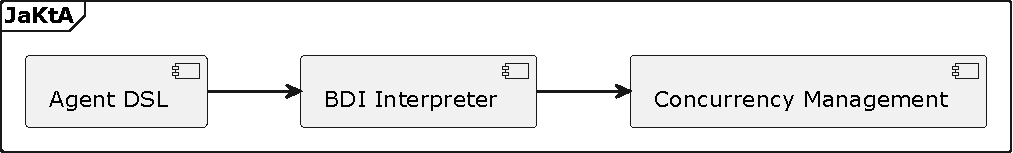
\includegraphics[width=\textwidth]{figures/sncs24/jakta_modules.pdf}
    \caption{\jakta{} modules and their relations. Arrowheads indicate dependencies (depends-on relationship).}
    \label{fig:framework-modules}
\end{figure}

Architecturally, the \jakta{} framework is composed by three main modules, namely:
%
\begin{enumerate}
    \item the \ac{DSL} module, which defines the syntax of the language;
    \item the \ac{BDI} interpreter, which governs the execution of agents and environments,
    regardless of the particular syntax used to define them;
    and
    \item the concurrency management module, which regulates runtime, concurrency, and scheduling aspects for
    any system run by the \ac{BDI} interpreter.
\end{enumerate}
%
As depicted in \Cref{fig:framework-modules}, the three modules are inter-dependent in a layered way:
the \ac{DSL} module is built on top of the \ac{BDI} interpreter,
which in turn is built on top of the concurrency management module.

The \ac{DSL} module is separate from the \ac{BDI} interpreter module
as it implements one possible syntax of many for \ac{BDI} \ac{MAS} specification.
%
Other languages could be plugged in the same \ac{BDI} interpreter,
for instance, the \jason{}'s parser can be, in principle, plugged on top of \jakta{}'s \ac{BDI} interpreter,
using the latter as engine.
%
Similarly, Scala developers may design a different internal \ac{DSL}
and plug it on top of the existing \ac{BDI} interpreter,
realising in shorter time a way to write \ac{BDI} agents in Scala.
%
Summarising, the neat modularisation of \ac{DSL} and \ac{BDI} interpreter opens to many possible \ac{BDI}
agents implementations, of which the current \jakta{} DSL is a possible instance.

\subsubsection{The \ac{DSL} module}

The \ac{DSL} module contains the syntactic constructs described in \Cref{subsec:language-description}.
%
Inside this module, \ac{BDI} abstractions from the interpreter module are mapped into the set of Kotlin classes and functions
enabling users to write \ac{MAS} specifications in Kotlin.
%

\subsubsection{The \ac{BDI} interpreter module}
\label{subsec:bdi-interpreter}

The \ac{BDI} interpreter is the component where the many abstractions of the \ac{BDI} model are reified into actual code,
giving semantics to the \ac{DSL} defined in \Cref{subsec:language-description}.
%
Put it simply, the \ac{BDI} interpreter module provides interfaces and implementations for the many abstractions
involved in the execution of a \ac{MAS}, there including the ones which are not visible in the \ac{DSL} syntax.
%
It provides ways to extend and inject abstractions which are meant to be personalised by \ac{MAS} developers
(such as actions, or environments),
and it encapsulates the abstractions which are not meant to be customised (e.g., the agents' control loop),
as per the best practices in the field~\cite{DBLP:journals/ase/DennisFWB12}.

\paragraph{Main abstractions}

In particular, the \ac{BDI} interpreter module provides interfaces and default implementations for the following abstractions:
%
\begin{itemize}
    \item beliefs and belief bases,
    \item goals,
    \item events and event pools,
    \item plans and plan libraries,
    \item intentions and intention pools,
    and
    \item side-effects (i.e., the admissible consequences of actions),
%    %
%    It also includes low-level abstractions such as agent identifiers.
%    %
%    All such abstractions are the basic bricks of the \ac{BDI} interpreter,
%    and they are \emph{not} meant to be customised by \ac{MAS} developers.
%    %
%    However, they could be reused by researchers willing to customise the \ac{BDI} interpreter itself.
%    %
%    Most notably, the module includes interfaces and abstract implementations for abstractions such as:
    \item (internal and external) actions,
    \item environments,
    \item agents,
    and
    \item message passing mechanisms.
\end{itemize}
%
In this case, the module prescribes what each abstraction may (or may not) do,
hence simultaneously enabling and constraining \ac{MAS} developers' customisations.
%
Most notably, all these abstractions are designed with immutability as a core design principle,
including those whose state must vary over time
through the \emph{copy-on-write} strategy.
%
This is key to support inspectability and reproducibility of the \ac{MAS} execution,
as well as to ease the introduction of parallelism in the execution of the \ac{MAS}.

\paragraph{Agent lifecycle and MAS}

Among the many abstractions provided by the \ac{BDI} interpreter module,
the most important ones are the \emph{agent lifecycle} and the \emph{\ac{MAS}}.
%
These are where all other abstractions are combined together to support the execution of \ac{BDI} systems.
%
In particular, the agent lifecycle is the component that dictates the execution of each single agent,
whereas the \ac{MAS} is the component which orchestrates the execution of all agents in the system,
as well as their interaction with (and through) the environment.

As far as the agent lifecycle is concerned,
this is the component that defines the control loop of each agent.
%
Assuming the internals of each agent include:
%
\begin{enumerate}
    \item a belief base,
    \item a plan library,
    \item a set of internal actions,
    \item an event pool,
    and
    \item an intention pool
\end{enumerate}
%
the default implementation of the agent lifecycle prescribes that
each iteration of each agent's control loop should encompass the following steps:
%
\begin{enumerate}
    \item percepts and messages for the current agent are collected from the environment;
    \item \label{lifecycle:bb-revision}
    the belief base is revised according to the new percepts and messages;
    \item events corresponding to added/removed beliefs or goals are generated and added to the current agent's event pool;
    \item \label{lifecycle:event-selection}
    one event is extracted (and removed) from the event pool;
    \item \label{lifecycle:plan-selection}
    relevant plans for the event are selected from the current agent's plan library;
    \item the guard of each selected plan is evaluated against the current agent's belief base;
    \item \label{lifecycle:applicable-plan-selection}
    one plan is selected for execution among the ones whose guard is satisfied;
    \item the plan is assigned to either a new or pre-existing intention in the current agent's intention pool;
    \item \label{lifecycle:intention-selection}
    one intention is selected for execution in the current agent's intention pool;
    \item \label{lifecycle:actuation}
    the next operation in the top-most plan of the selected intention is executed, and then discarded;
    \item any side-effect produced by the execution of the operation is collected and returned as output of the single iteration of the control loop.
\end{enumerate}

Most notably, steps
\ref{lifecycle:bb-revision},
\ref{lifecycle:event-selection},
\ref{lifecycle:plan-selection},
\ref{lifecycle:applicable-plan-selection},
and
\ref{lifecycle:intention-selection}
are designed to be customisable by users.
%
It is also with mentioning that step~\ref{lifecycle:actuation} is where the execution of internal or external actions occurs.
%
So, this is where the execution of custom \ac{OOP}/\ac{FP} code is performed.
%
As a byproduct, actions may provoke side-effects, whose management is described in the following.

The \ac{MAS} component is where the lifecycles of all agents in a system are tied together and coordinated,
along with any computational activity involving the environment (e.g., message dispatching).
%
Put it simply, this component is in charge of keeping track of which and how many agents compose the system.
%
For each of these, the \ac{MAS} shall govern the unlimited repetition of their control loop,
following the aforementioned steps.
%
In which order the many control loops of the many agents are interleaved is a matter of implementation%
---and several implementations are available in \jakta{},
as enabled by the concurrency management module (cf. \Cref{sec:concurrency-module}).

Regardless of the particular order by which agents' control loops interleave,
the \ac{MAS} is responsibile to ensure the reification in the environment
of any side-effect produced at each iteration of any agent's control loop.
%
There, side-effects essentially consist of message exchanges among agents,
or changes in the environment's data.
%
Of course, the actual semantics of side-effects reification depends on the particular implementation of the environment.

\paragraph{Environment and message-passing mechanism}

The environment is a first-class abstraction in \jakta{}.
%
However, the notion of environment is highly dependant on the particular application domain at hand.
%
Hence, we designed a minimal environment which developers may customise depending on their need
with the following responsibilities:
%
\begin{itemize}
    \item keeping track the agents in the system;
    \item governing the perception of each agent by deciding which percepts to deliver to each agent;
    \item governing the actuation of each agent by making external actions available to each agent;
    \item governing the communication among agents by deciding how messages are delivered to each agent;
    \item enabling the stigmergic interaction among agents by making the environment's data available to each agent.
\end{itemize}

Of course, \jakta{} also provides a default implementation of the environment,
very simple and general purpose, where agents can perceive knowledge, act on its state, or send messages to other agents%
---assuming that other agents are running inside the same OS process.

To support inter-process or inter-machine communication, users must provide their custom environment implementation.
%
This design choice was mainly driven by flexibility,
especially related to network concerns;
in fact,
different users may be willing to leverage different communication protocols.
%
%For instance, users may be willing to distribute their \ac{MAS} via HTTP, or via a message queue%
%---possibly backed by some message-broker leveraging the XMPP or AMQP protocols.

\paragraph{Actions and side-effects}

Just as for other notable \ac{BDI} languages, agents' specification in \jakta{} are \emph{declarative},
%
%The \ac{DSL} mostly exploits functional and object-oriented programming constructs to provide such declarativity.
%
%However,
except in the case of (internal and external) actions.
%, the role of functional, object-oriented, or imperative programming is different.

To agents, actions are -- conceptually -- the way to make things happen (either in the environment or on themselves).
%
However, ``making things happen'' may imply expressing computations which are not convenienty represented via declarative constructs.
%
There, actions aim to bridge the gap between the declarative world of \ac{BDI} agents and mainstream programming constructs.
%
Thus, actions are the means by which agents can declaratively invoke functional, object-oriented, or imperative code.

\begin{figure}
    \centering
    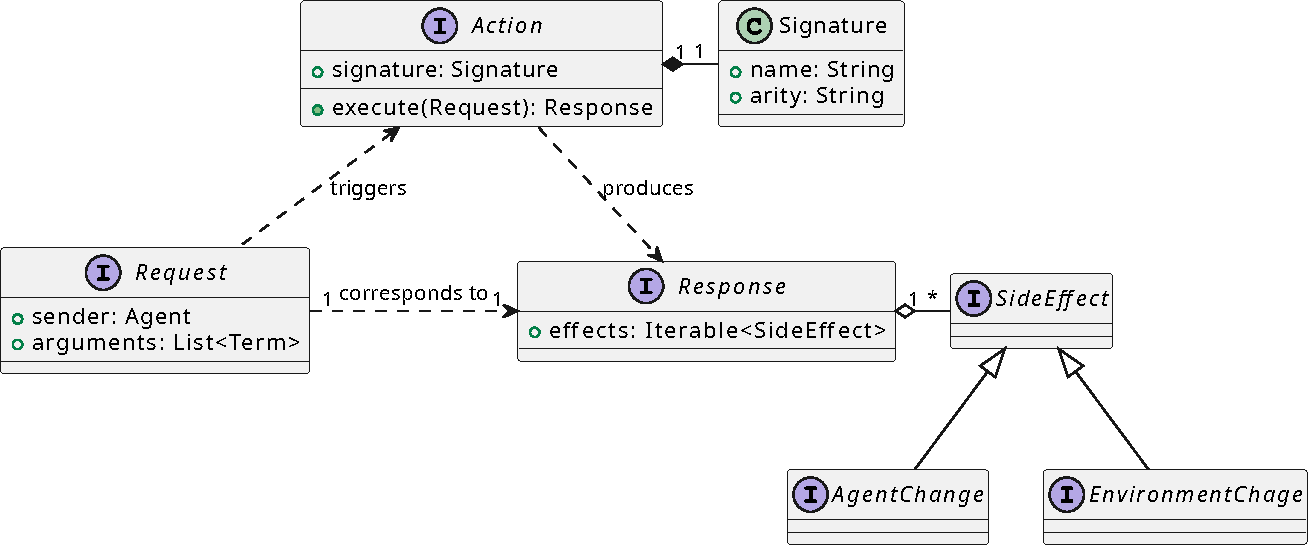
\includegraphics[width=.7\textwidth]{figures/sncs24/action_interface.pdf}
    \caption{\jakta{} Action interface hierarchy.}
    \label{fig:action-hierarchy}
\end{figure}

Technically speaking, actions are arbitrary functionalities, written in Kotlin, which may provoke side-effects%
---either on the agent itself, or on the environment.
%
To support this feature, the \ac{BDI} interpreter module provides ad-hoc type hierarchy, represented in \Cref{fig:action-hierarchy}.
%
Actions are functional interfaces triggered by a request (coming from an agent) and producing a response in return.
%
Each action as a signature, which denotes the name and arity by which it is known to agents.
%
Each request contains a reference to the triggering agent, and a list of actual arguments.
%
Each response contains a list of side-effects, each one describing an edit to be performed on the agent's state, or on the environment.
%
Admissible changes to the agent's state include: addition or removal of beliefs, goals, plans, or intentions, as well as the stopping or pausing of the agent itself.
%
Admissible changes to the environment include: addition or removal of agents, update of data in the environment, or sending of messages to other agents.
%
The way by which the action produces the response is up to the action implementors,
which may exploit Kotlin to do whatever they want.



\subsubsection{The concurrency management module}
\label{sec:concurrency-module}

The concurrency management module aims at letting users customise the concurrency model of their \ac{MAS}.
%
To put it simply, the module lets users choose \emph{how} agents are scheduled and executed%
---i.e., how they can be allocated on top of threads.
%
One may for instance choose to have a single thread per agent, or to have a thread pool shared by all agents,
depending on the application at hand.
%
In the second case, implementers may also choose the atomicity of agents' control loops:
they may for instance make the single iteration of the loop atomic,
hence allowing multiple agents interleave their execution in the most fine-grained way possible.
%
The module also takes care of virtualising relevant aspects related to agents execution, such as the flow of time.
%
For the sake of conciseness,
we do not details in this work all the concurrency models supported by \jakta{}'s \ac{BDI} interpreter;
the interested reader may refer to the documentation of the framework for further details~\cite{Baiardi2023}.
% \dpnote{qua mettere un link, eventualmente anche a un readme del cazzo, o alla tesi di martina se è in inglese, poi a regime mettiamo AAMAS}

One key take-away here is that the \ac{BDI} interpreter is built on top the concurrency module.
%
Decoupling the BDI interpreter and the concurrency modules is based on the idea that the
former decides \emph{what} to execute,
leaving to the latter the decision on \emph{how} to execute it.
%
% For instance, a simple concurrency model that continuously schedules agents in a round-robin fashion will invoke the execution of a reasoning cycle iteration for each agent, one after the other, in a loop.

\section{\jakta{} in practice: running example}
\label{sec:running-example}

In this section, we show how \jakta{} compares with a reference AOP technology
(\jason{})
through a running example in terms of
%
\begin{inlinelist}
    \item multi-paradigm integration, and meta-programming,
    \item abstraction, re-use and type safety; and
    \item tooling and ecosystem.
\end{inlinelist}

\paragraph{Learning \jakta{}}

For the sake of conciseness,
we keep the example deliberately minimal.
%
% The choice of $N \times N$ TicTacToe is deliberately simple, as it let as concisely demonstrate the benefits of the internal \ac{DSL} approach.
%
The full code of the example is available on a public repository\footnote{
    \url{https://github.com/jakta-bdi/jakta-examples}
}.
%
In the same repository,
the reader can find several running examples of \jakta{} applications,
which can be used as a starting point to learn the framework.
%
Since \jakta{} is Kotlin-internal \ac{DSL},
knowledge of the host language is needed to be proficient with the framework.
%
For those who do not know Kotlin, we recommend to first learn Kotlin through the official documentation\footnote{
    \url{https://kotlinlang.org/docs/home.html}
},
exercising with the Kotlin Koans Online\footnote{
    \url{https://play.kotlinlang.org/koans/overview}
}, then move to our example repository to learn Jakta.


\subsection{Reference scenario}\label{sec:reference-scenario}

We selected a scenario to highlight the benefits of paradigm blending:
we want to write a multi-agent modelling a TicTacToe match played on a $N \times N$ board,
where $N$ is only known at runtime.
%
The agent may perceive the environment (the board) via percepts of the form \prologInline{cell(X, Y, Z)},
where \prologInline{X} and \prologInline{Y} are the coordinates of the cell,
and \prologInline{Z} $\in$ \{\prologInline{e}, \prologInline{x}, \prologInline{o}\} is the symbol contained in the cell.
%
The agent may also perceive the beginning of a turn via the \prologInline{turn(x)} (resp., \prologInline{turn(o)}) percept,
and may place a symbol in a cell of the environment using the \prologInline{put(X, Y, Z)} \emph{external} action---which also passes the turn.
%
The agent's play strategy is the following:
%
\begin{inlinelist}
    \item if there are $N$ of your (resp. the other player's) marks aligned in a row, declare victory (resp. defeat);
    \item if there are $N-1$ of your (resp. the other player's) marks aligned
    and the $N^\text{th}$ cell in the same direction is empty,
    write your mark in that cell;
    \item put a cross in random empty cell.
\end{inlinelist}

There are four alignment directions, so the agent's belief base can host:
\\
\begin{minipage}[c]{\textwidth}
    \prologImport[linerange={1-4},basicstyle=\footnotesize\ttfamily]{listings/sncs24/tictactoe-directions-meta.asl}
\end{minipage}
%
The critical part of the scenario, however, is dealing with a grid of \emph{unknown size}.
%
For a simple $3 \times 3$ case, the problem can be dealt with via four couples of rules in the form:
\\
\begin{minipage}[c]{\textwidth}
    \prologImport[linerange={5-8},basicstyle=\footnotesize\ttfamily]{listings/sncs24/tictactoe-directions-meta.asl}
\end{minipage}
%
where meta-variable \meta{alignment} can be:
\pl{vertical},
\pl{horizontal},
\pl{diagonal},
and \pl{antidiagonal},
while \meta{dx},
\meta{dy} are in 1, 0, or -1.
%
Under these premises, for a $3 \times 3$ simplified scenario,
the plans dealing with victory, loss, and random choice may be written in \jason{} as:
\\
\begin{minipage}[c]{\textwidth}
    \prologImport[linerange={1-3},basicstyle=\footnotesize\ttfamily]{listings/sncs24/tictactoe-plans.asl}
\end{minipage}
%
whereas plans making the final move can be written as:
\\
\begin{minipage}[c]{\textwidth}
    \prologImport[linerange={5-7},basicstyle=\footnotesize\ttfamily]{listings/sncs24/tictactoe-plans.asl}
\end{minipage}
%
Plans impeding the victory of the opponent would be very similar.

This way of writing plans, however, does not scale well with the size of the board:
a $N \times N$ board would count $2N + 3$ plan statements with a guard mentioning $N$ cells.
%
%The way these situations are usually dealt with is by creating AOP code generators in other languages, a condition that blending paradigms can prevent.
%
There are no good strategies to handle these situations in pure \jason{} (i.e. without using external tools to generate code), while they can be managed by relying on alternative paradigms in \jakta{}.

\subsection{Multi-paradigm integration and meta-programmability}\label{subsec:behaviour-parametrization}

The same application in \jakta{} could be created by defining a
\emph{parametric} \ac{MAS} via an ordinary Kotlin function with a parameter:
\\
\begin{minipage}[c]{\textwidth}
    \kotlinImport[linerange={1-9},basicstyle=\footnotesize\ttfamily]{listings/sncs24/tictactoe-mas.kt}
\end{minipage}
%
The function declares a \ac{MAS} whose environment of type \kotlinInline{GridEnvironment}
of size \kotlinInline{gridSize} supporting an external action \kotlinInline{Put}.
%
The \kotlinInline{Put} action is defined as a Kotlin object, in another file,
and extends the \kotlinInline{AbstractExternalAction} provided by the framework:
\\
\begin{minipage}[c]{\textwidth}
    \kotlinImport[linerange={62-70},basicstyle=\footnotesize\ttfamily]{listings/sncs24/tictactoe-mas.kt}
\end{minipage}
%
The action takes three arguments, which are the position where to insert the mark and the mark itself.
%
Finally, it update the environment's data, by the means of the \kotlinInline{updateData} environment's side effect.

The two players are agents returned by the \kotlinInline{player} extension function:
%
\\
\begin{minipage}[c]{\textwidth}
    \kotlinImport[linerange={11-29},basicstyle=\footnotesize\ttfamily]{listings/sncs24/tictactoe-mas.kt}
\end{minipage}
%
Notably, the function exploits multiple paradigms to construct agent specifications via AOP meta-programming.
%
For instance,
predicate \pl{aligned/1} is defined in a \kotlinInline{forEach} loop,
while predicates \pl{vertical/1}, \pl{horizontal/1}, and (\pl{anti})\pl{diagonal/1} are defined
by calling the \kotlinInline{alignment} function,
which parametrically builds rules to compute alignments along the four major directions:
\\
\begin{minipage}[c]{\textwidth}
    \kotlinImport[linerange={31-43},basicstyle=\footnotesize\ttfamily]{listings/sncs24/tictactoe-mas.kt}
\end{minipage}
%
With no paradigm blending,
based on the bare \agentspeak{} syntax,
the rules would have needed to be copied and modified to support multiple cases instead.

Plans are defined by means of Kotlin functions as well:
\jakta{} plans can have names, meta-parameters, and leverage decomposition.
%
For instance,
victory and defeat detection are implemented with functions parametric in the symbol of the player and size of the grid:
\\
\begin{minipage}[c]{\textwidth}
    \kotlinImport[linerange={45-48},basicstyle=\footnotesize\ttfamily]{listings/sncs24/tictactoe-mas.kt}
    % \kotlinImport[linerange={33-38}]{listings/sncs24/tictactoe-mas.kt}
\end{minipage}
% \\
% \begin{minipage}[c]{\textwidth}
%     \kotlinImport[linerange={35-36}]{listings/sncs24/tictactoe-mas.kt}
% \end{minipage}
and both rely on a generic \kotlinInline{detect} function implementing a \emph{template plan}:
\\
\begin{minipage}[c]{\textwidth}
    \kotlinImport[linerange={49-50},basicstyle=\footnotesize\ttfamily]{listings/sncs24/tictactoe-mas.kt}
\end{minipage}
%
%====================================
% SB: Ho rimosso questo perché mi sembra che in realtà la abbiamo messa alla fine quindi mi stonava
%====================================
% A similar technique has been used to build plans
% detecting victory and defeat,
% which we omit for the sake of brevity.
%
Finally,
we show how \emph{plan generation} can be realised in \jakta{}
by showing the implementation of \kotlinInline{makeWinningMove}:
\\
\begin{minipage}[c]{\textwidth}
    \kotlinImport[linerange={52-55},basicstyle=\footnotesize\ttfamily]{listings/sncs24/tictactoe-mas.kt}
\end{minipage}
%
There, \kotlinInline{gridSize} plan statements are generated,
one for each possible position of the empty cell in a line containing $N-1$ cells with the same mark.
%
Once again, the definition is parametric in the size of the grid and the symbol of the current agent.
%
In this way, the \jakta{} code would work with all possible values $N>0$,
whereas the corresponding \agentspeak{} code would need to be tailored on a single value of $N$.

We believe that reusable units of agent behaviour
such as template plans and plan generation,
made possible by intertwining multiple paradigms,
promote abstraction, reuse, and allow for improved code-organization.

\subsection{Code organisation, reuse, and type safety}

Proper organisation is important to the understandability and extensibility of any program.
%
For instance, in our example, separating the belief base from the plan library
may be useful to change the latter in order to implement different strategy.
%
The main reuse technique in \jason{} (similar for many other external AOP \acp{DSL}) is plain file inclusion,
performed with statements of the form {\prologInline{include("path/to/file.asl")}}.
%
The mechanism is simple, but arguably limited and relatively unsafe,
as the actual result of the inclusion will be known at runtime.
%

Instead, \jakta{} inherits the abstraction mechanisms of Kotlin:
programs can be suitably split into different pieces,
at different levels of granularity
(package, file, class, function).
%
Pieces may be either individual beliefs, plans, actions, or agents, or even groups of them.
%
Furthermore, \jakta{}'s (Kotlin's) reusable abstractions are \emph{type-safe}:
one cannot, for instance, include a belief where a plan is expected,
and consistency is verified at compile time by the Kotlin compiler.

\subsection{Tooling and ecosystem}

\begin{figure}[t]
    \centering
    \caption{
        IDE support for \jason{} and \jakta{} compared Visual Studio Code (top)
        and IntelliJ Idea (bottom).
        By inheriting the tools made for Kotlin,
        \jakta{} is fully supported in both IDEs with no need for additional development or maintenance.
    }
    \label{fig:ca}
    \subfloat[\jason{} on Visual Studio Code]{
        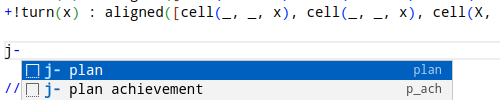
\includegraphics[width=.48\linewidth]{figures/sncs24/code-jason.png}
        \label{fig:code-jason}
    }
    % \hfill
    \subfloat[\jakta{} on Visual Studio Code]{
        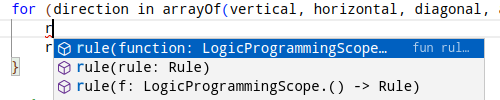
\includegraphics[width=.48\linewidth]{figures/sncs24/code-jakta.png}
        \label{fig:code-jakta}
    }
    \\
    \subfloat[\jason{} on IntelliJ Idea]{
        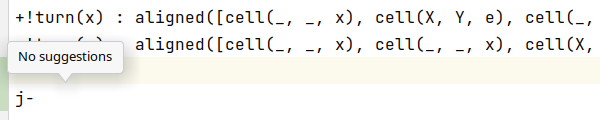
\includegraphics[width=.48\linewidth]{figures/sncs24/idea-jason.png}
        \label{fig:idea-jason}
    }
    % \hfill
    \subfloat[\jakta{} on IntelliJ Idea]{
        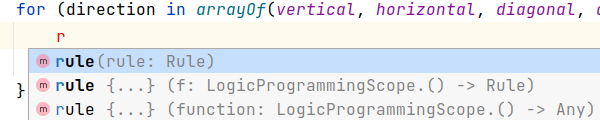
\includegraphics[width=.48\linewidth]{figures/sncs24/idea-jakta.png}
        \label{fig:idea-jakta}
    }
\end{figure}

An indirect benefit of internal \acp{DSL} is the availability of inheriting the rich ecosystem of tools of the host language.
We quickly exemplify in \Cref{fig:ca}
comparing how \jakta{} and \jason{} are supported by two commonly used IDEs:
Visual Studio Code (VSCode) and IntelliJ Idea.
%
We install, in both cases, the latest version of the \jason{} and Kotlin plugins;
notably, we developed nothing specific for \jakta{},
so everything that is displayed came with no development and maintenance cost.
%
As the figure shows,
we get code highlighting and content assist for both languages in VSCode,
although, thanks to Kotlin's type system,
we obtain better completion suggestions.
It is also worth noting that the suggestions for \jason{} are in the form of code snippets and have no real contextual relevance.
%
On IntelliJ Idea, however, we have no highlighting or assist of any kind for \jason{}
beyond the tools the IDE provides for plain text files:
in fact, no \jason{} plugin for Idea exists,
users coming from that IDE need to adapt to a new one,
or developers need to invest time and resources into developing one.
%
Oppositely, \jakta{} is fully supported in any IDE featuring Kotlin support
(at the time of writing, this includes VSCode, Idea, Android Studio, Eclipse, and Atom\footnote{
    \href{https://archive.is/eXUuT}{https://kotlinlang.org/docs/kotlin-ide.html}
}).

Additionally,
leveraging Kotlin as host language allows \jakta{} code to be smoothly embedded in Android applications.
%
The TicTacToe example described above has also been tested on Android\footnotemark, as demonstrated by \Cref{fig:tictactoe-android}.
%
\footnotetext{code available at: \url{https://github.com/jakta-bdi/jakta-android-example}}
%
\jakta{} is available on Maven Central,
and can thus be imported as an ordinary dependency in any Android project,
at the cost of a single line in the projects' Gradle build file.

\begin{figure}
    \centering
    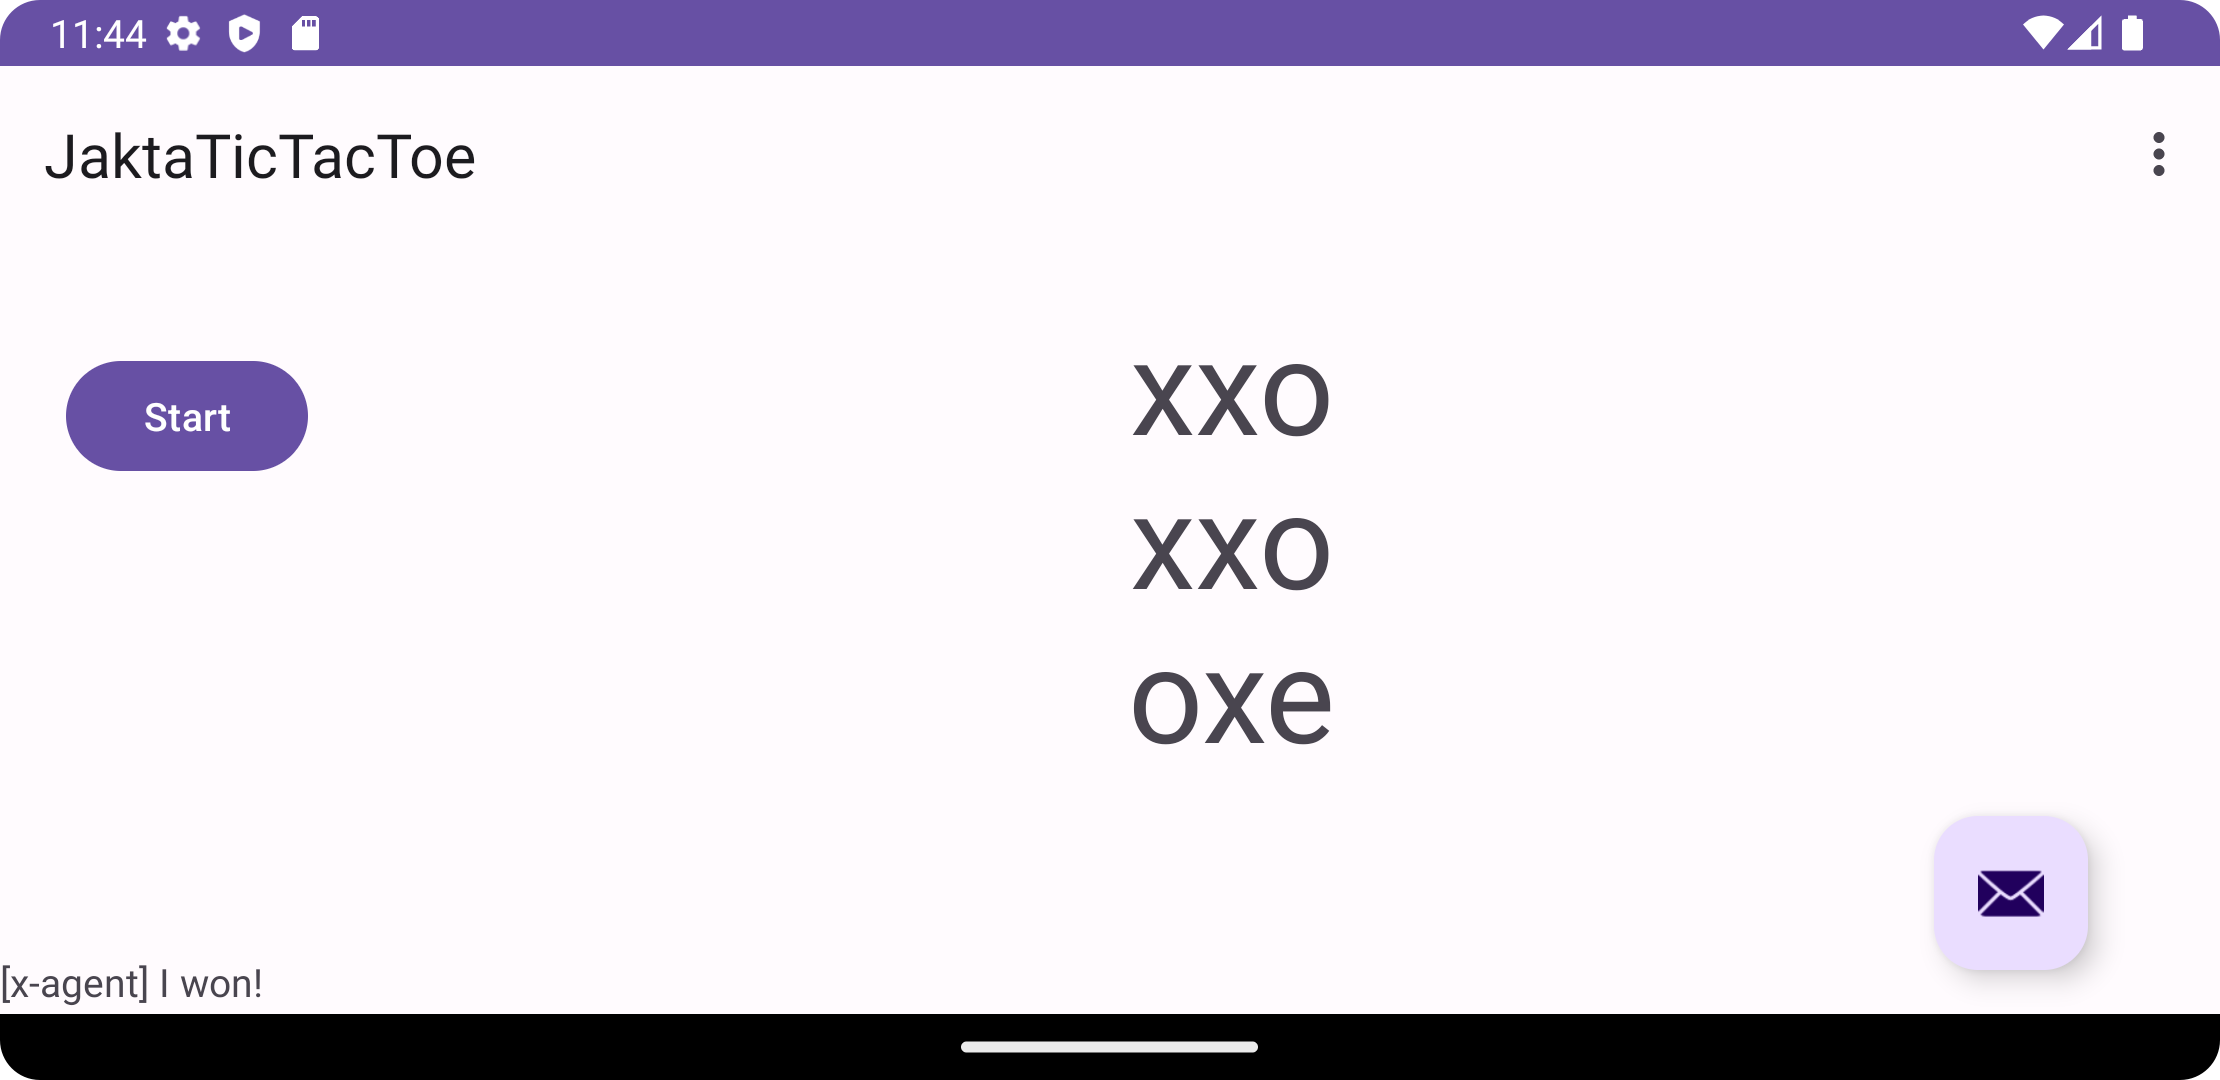
\includegraphics[width=0.5\linewidth]{figures/sncs24/tictactoe-android.png}
    \caption{The TicTacToe \ac{MAS} running on Android.}
    \label{fig:tictactoe-android}
\end{figure}


\section{Conclusion, limitations, and future work}\label{sec:conclusion}

In this chapter,
we introduced \jakta{}:
an internal Kotlin \ac{DSL} for \ac{BDI} agent programming that strives to achieve
true paradigm blending of \ac{AOP}, \ac{OOP}, and \ac{FP}
within a mainstream general-purpose programming language.
%
We show how \jakta{} can be used to implement a simple \ac{BDI} agent
and how paradigm blending can be used to achieve improved modularity
and reusability,
including reusable \ac{BDI} elements,
thus providing value to the authors of AOP software.
%
Moreover,
we show that,
with no need for dedicated components or tools,
and thus with no additional development and maintenance cost for the language developers,
\jakta{} is already supported by most popular IDEs,
as it can rely on the existing infrastructure of its host language.
%
Additionally,
we argue that \jakta{} could enable more developers to get in touch with AOP,
since it does not require newcomers to learn a new syntax or adopt new tools.

\jakta{} is thus a first step towards the full integration of \ac{AOP}
in a modern programming language,
achieving paradigm blending.
%
This research direction opens up many interesting problems that can be explored going forward:
in this section,
we will thus start from the current limitations of \jakta{}
to discuss future work.

\paragraph{DSL Syntax}

Since the target users of \jakta{} are both
experienced agent developers familiar with the \ac{BDI} style of programming
and novice programmers coming from traditional \ac{OOP} languages,
when designing the \ac{DSL} syntax for \jakta{}
we tried to balance between familiarity with existing agent technologies and expressiveness.

Given its popularity in the community,
we draw inspiration from \jason{},
producing a syntax with several similarities.
%
The differences are partly deliberate and partly
consequential to the syntactic boundaries imposed by
the host language.
%
For instance, only a small subset of symbols representing operators in Kotlin can be customised:
as an example,
while the symbol \kotlinInline{!} is an overridable operator,
the symbol \kotlinInline{?} cannot be used nor defined.

At the same time, we believe these limitations allowed us to use explicit keywords
such as \kotlinInline{achieve} and \kotlinInline{test}
over dedicated symbols that could be considered cryptic for novice users.
%
More generally,
in many cases, we had to pick syntactical design choices harmonizing the \jason{}'s syntax with the Kotlin one.
%
As a result, the \jakta{} syntax is more verbose compared to \jason{}'s,
but we believe that this is a reasonable trade-off
to get the benefits of using Kotlin as hosting language.

As the \ac{DSL} module is independent of the interpreter,
we plan to experiment with the syntax in order to refine the current version
and make it more pleasant to use.
%
We will thus be open to collecting feedback from other research groups experimenting with \jakta{}
as well as from students approaching \ac{AOP} for the very first time.

We also believe that the freedom given by the \jakta{} \ac{DSL} implementation
could allow for different \textit{dialects} to co-exist,
building on the same interpreter.
%
This is especially interesting when considering porting \jakta{}
to different platforms other than the \ac{JVM},
a matter deserving its own paragraph.

\paragraph{Kotlin multiplatform support}

Although the multiplatform targeting supported by Kotlin
is among the reasons why the technology was chosen,
the current implementation of \jakta{} is available only for the \ac{JVM}.

In the future,
we plan to fully leverage this capability,
thus enabling the exploitation of a single language and interpreter for running \ac{BDI} systems
inside web browsers (Kotlin/JavaScript),
mobile (Kotlin/Android, Kotlin/Native for iOS),
wearable and low-power (Kotlin/Native),
and general-purpose (Kotlin/JVM) applications,
retaining cross-platform interoperability.

This would make \jakta{} a desirable solution for emerging scenarios with heterogeneous devices,
especially when this feature is combined with the freedom of customisation
given by the fact that most architectural components can be swapped with custom implementations.
%and we believe that developers could leverage the \textit{pluggability} features of \jakta{}
%to implement even more idiomatic APIs for the target languages,
%thus easing the use of \ac{AOP} not only for Kotlin developers,
%but also for developers more acquainted with working on other platforms and languages.

\paragraph{Paradigm blending}

Approaching the interesting problem of paradigm \textit{blending},
we mainly considered the benefits that mixing \ac{OOP} and \ac{FP} constructs
could bring to the development of multi-agent systems.

There are, however, some limitations in the way \jakta{}
handles blending that might be interesting to address with further iterations on the language.
%
% \dpnote{le seguenti erano due frasi prive di senso in inglese. Non banale capire cosa si volesse dire. Ho provato a riscriverlo. Pregasi rileggere e, in caso, seccare o fare rollback.}
For instance, some \acs{BDI} languages such as \jason{} and \astra{}
introduce syntactic constructs akin to those of imperative languages
(e.g., \texttt{for}, \texttt{foreach}, and \texttt{if} statements)
to ease the definition of procedural plans,
as an attempt to become more developer-friendly.
%
These constructs are not part of the common formalization of \ac{BDI} languages.
%
They are \textit{syntactic sugar} aimed to reduce the verbosity of plans,
or the need to define auxiliary actions.

As the \jakta{} \acs{DSL} is embedded in the Kotlin language,
agents specifications
-- and, in particular, plans definitions --
may contain Kotlin's imperative constructs too%
---such as \kotlinInline{for} loops, and \kotlinInline{if} or \kotlinInline{when} statements
(cf. \Cref{subsec:behaviour-parametrization} for an example on \emph{meta-programmability}).
%
However, this may produce surprising behaviours in the eyes of inexperienced developers.
%
In fact,
in our \acs{DSL},
any piece of Kotlin code just aims at \emph{building} the declarative specification of a \acs{MAS}%
---there including agents and plans.
%
Yet, such specification may only contain \agentspeak{}-compliant, declarative constructs,
as those are the only ones the \jakta{} interpreter supports.
%
The code used within a \acs{MAS} definition is executed only after
the \acs{MAS} structure has been assembled,
not when the interpreter runs the \acs{MAS} itself.
%
Although this is arguably a desirable effect,
we reckon that it may be astonishing for novice developers,

Along this line,
it would be interesting to explore whether
\jakta{}'s \acs{BDI} interpreter can be extended to natively support
as one further step towards full feature equivalence w.r.t. \jason{} or \astra{}.

At the same time,
in this work,
we do not explore what benefits an \ac{AOP} portion of code could bring
to the development of an \ac{OOP}/\ac{FP} project.
%
We believe that, to achieve true blending,
it might be interesting to explore this option more in depth;
as it could bring to even more intertwined connections among paradigms.
%
For instance,
a bunch of agents may be employed to cooperatively execute a parallelisable task,
whose result may be returned asynchronously to the \ac{OOP}/\ac{FP} world
%to compute an asynchronous result
(e.g., via promises).
% thus interacting with the object-oriented portion of a program.
%
Despite being technically straightforward,
such a functionality would come with many challenging theoretical implications%
---e.g., when should each agent terminate?
when should the \ac{MAS} terminate?
what is the best way to propagate results back to the \ac{OOP}/\ac{FP} realm?
%
At the same time,
we believe features of this kind might strengthen the link between paradigms,
and truly support \textit{blending}, giving even more choices
to developers in picking the paradigm, and the abstraction,
they find themselves more comfortable with for each specific task.

\paragraph{Debugging}

Among the main benefits of choosing an internal \ac{DSL},
we mentioned the possibility of reusing the tools
available for the host language without the need to implement
new ones from scratch.
%
This includes debugging tools,
which are essential for robust software engineering.

While \jakta{} programs can already be debugged through the existing the Kotlin debuggers,
available for many mainstream \ac{IDE},
the abstractions observed inside the inspector are those internal to Kotlin.
%
This means, for instance,
that when stopped on a breakpoint the tool will show Kotlin objects and references
instead of \jakta{}'s higher-level \ac{AOP} constructs.

Moreover, using breakpoints is trickier than in ordinary Kotlin,
a breakpoint positioned without care might be triggered at a surprising moment
(typically, before the \ac{MAS} is even started).
%
This is a consequence of the strategy used to construct the \ac{DSL}:
we heavily rely on lambda expressions
whose code is evaluated at \ac{MAS} \emph{construction}
to produce an executable system whose actual execution is performed later by the interpreter,
so breakpoints set on those lines will be triggered at construction time%
---indeed, it is not a coincidence that internal \acp{DSL} in Kotlin are
called ``type-safe builders''.

A third issue that makes the native Kotlin debugger suboptimal concerns the stack inspection.
%
As the abstractions visualised in the tool are those of the host language,
so the stack frames will be those native of Kotlin,
producing stacktraces harder to inspect than those mapping \ac{AOP} abstractions directly.

Debugging of BDI agents is indeed an open issue in the community,
different platforms adopt different approaches;
as an example, \jason{} famously offers a graphical interface
for a \textit{mind inspector}
showing the current beliefs and intentions that are
present in the agent's ``mind'' during execution.

We believe that,
although initial debugging support
in the form of the native Kotlin debugger is useful,
it might be interesting to investigate how to support the developers
producing more meaningful error messages and dedicated debugging tools
that preserve the abstractions of the agent program.

\paragraph{Concurrency management}

Concerning runtime behaviour,
\jakta{}'s architecture has been designed to separate the concurrency model
from the agent specification.

Currently, we only support a handful of alternatives,
including the widely used \acs{1A1T} execution strategy that runs
agents concurrently on separate threads (one per agent),
as well as \acs{AA1T}, where the whole MAS runs on a single thread.
%
As the latter may be useful for debugging and simulation scenarios,
\jakta{} also supports a virtualised-time mode,
where the flow of time is detached from the real time.
% \dpnote{che è la discrete-time mode? Intende la modalità dove il tempo è virtuale?}

Accordingly,
the concurrency module of \jakta{} enables exploring and comparing the impact of concurrency abstractions
on the design of a \ac{MAS}.
%
Along this line, we plan to
%
\begin{inlinelist}
    \item  widen the set of execution strategies supported by \jakta{},
    possibly including more advanced ones such as \acs{AA1E},
    and to
    \item investigate how \jakta{} can be integrated with mainstream simulation and concurrency frameworks
    to provide better support to the development of simulated or parallel \ac{MAS}.
\end{inlinelist}

\paragraph{Distributed Multi-Agent Systems and Messaging}

Many applications in the field of \ac{MAS} are distributed systems,
where agents move or communicate across networked computers.
%
At the time of writing, though,
\jakta{} does not support agents communicating or moving across the network,
as the only message-passing mechanism currently implemented is in-process.

Although we acknowledge this limitation,
\jakta{} already supports full customisation of the message-passing mechanism%
---a feature that we plan to exploit soon
by including a \emph{distributed} message-passing mechanism in the
default distribution of our framework.

The same goes for the limited set of performatives that are currently supported:
a richer set is fundamental to support the adoption of \jakta{} by \ac{MAS} developers;
our goal mid-term is to support the same set of performatives supported by \jason{}. %in the coming versions.

In the long run,
we may also modularise the \ac{ACL} supported by \jakta{},
paving the way towards the possibility of supporting multiple \ac{ACL}.
% This would make customisation of the message-passing mechanism
% even easier from the developers' point of view.

% \sbnote{Over promising?}

\paragraph{Action libraries}

For any new programming framework, the surrounding ecosystem of libraries is essential to thrive.
%
\jakta{} benefits from the possibility of integrating easily with the Kotlin ecosystem and libraries.

At the same time,
we understand that \acp{MAS} developers may benefit from the existence
of a rich standard library of internal actions,
as well as from sets of easily importable and reusable external actions
for specific problems (e.g., integrating with Web services or databases).

Creating and distributing such libraries of actions is trivial in \jakta{},
as developers can directly reuse the build tools and software repositories commonly used
in the development of vanilla Kotlin programs,
such as Gradle and Maven Central.

Currently,
\jakta{} is shipped with a very minimal core set of features that we plan to expand over time .
%
Moreover,
\jakta{} is an open-source project:
we warmly welcome contributions,
including those in the form of libraries,
and we plan to collect and promote projects affiliated with and extending \jakta{},
hence encouraging the creation of an active community.

\paragraph{Performance evaluation and optimisation}
In this chapter, our focus is on a software engineering perspective,
discussing the application of internal \acp{DSL} to \ac{BDI} agent programming,
demonstrating feasibility, design challenges, and benefits of the approach.
%
However, for the tool to be practically useful,
future work need to evaluate its performance in detail.
%
We internally conducted some initial profiling,
discovering that (expectedly) most of the performance burden is due to \jakta{}'s immutable-by-default design,
which purposedly trades performance for thread-safety by leveraging on copy-on-write data structures%
---in order guarantee the agents' interpreter works correctly regardless of the concurrency model of choice.
%
We believe that performance can still be heavily improved,
thus, we are delaying performance measurement until a reasonably optimised version of the tool is ready.
%
In future work,
we will first analyse in detail and tackle the performance bottlenecks of \jakta{},
then run benchmarks to compare the performance of \jakta{} with other \ac{BDI} tools,
primarily \jason{}.

\chapter{External Concurrency in BDI Framework Implementations}

This chapter focuses on a practical and often overlooked question: 
how do existing \ac{BDI} framework implementations 
manage concurrency in real deployments. 

We analyse the \ac{BDI} frameworks (see \Cref{subsec:agentspeak-frameworks}) whether, 
and to what extent, they 
expose, 
configure, 
or hide the mapping between agent abstractions 
and the underlying concurrency primitives.
%
In this chapter we refer to the mapping between \ac{BDI} abstractions 
and the underlying concurrency primitive
as the \emph{concurrency model} of the framework.

We use the term ``\emph{external} concurrency'' to denote the policy 
that maps whole agents (their control loops) 
onto platform-level concurrent constructs such as 
threads, 
processes, 
or event loops. 
%
External concurrency complements the ``\emph{internal} concurrency'' of an agent 
(i.e., how an agent interleaves or parallelises its own 
sensing, 
deliberation, 
and acting stages), 
and we claim that the interaction between the two 
has important practical consequences for performance, 
determinism, 
and reproducibility.

The goal of this chapter is software engineering-oriented: 
we systematically examine a representative set of \ac{BDI} frameworks to understand
\begin{inlinelist}
    \item whether they make the external concurrency model explicit or configurable,
    \item and
    \item which primitives they rely upon (one-thread-per-agent, shared thread-pools, single-threaded event loops, etc.).
\end{inlinelist}

Our analysis produces a taxonomy of external concurrency models, 
a classification of notable \ac{BDI} implementations against this taxonomy, 
and a set of practical engineering recommendations for the development of \ac{BDI} technologies, suggesting to make concurrency choices visible and controllable.

We start this chapter describing the terminology we rely on (Section~\ref{sec:background}) and then present the taxonomy of external concurrency models (Section~\ref{sec:taxonomy}). Section~\ref{sec:comparison} applies the taxonomy to a set of real frameworks and discusses practical trade-offs; Section~\ref{sec:discussion} draws lessons and recommendations for framework design and use.
%
We analyse concurrency models commonly adopted in modern software development,
then (\Cref{sec:taxonomy}) we discuss how agents (and their internal components) can be mapped onto them,
evaluating the pros and cons.
%
In \Cref{sec:comparison} we evaluate several \ac{BDI} technologies from the \ac{AOP} community from a concurrency-related perspective,
eliciting the available concurrency models and their degree of configurability.
%
Finally,
in \Cref{sec:discussion} we elaborate on the importance of configurable concurrency models
well-separated from the agent's behaviour specification.

\section{Background}\label{sec:background}

In this section,
we first recall basic notions frame the concepts of \emph{internal} and \emph{external} concurrency,
then
look at the existing work specifically addressing concurrency in the context of \ac{BDI} \ac{AOP},
thus framing our contribution with respect to the state of the art.
%
Then
we discuss the lower-level concurrency abstractions required to understand the remainder of the chapter.

\subsection{Internal vs.\ External Concurrency}

A multi-\ac{BDI}-agent system can be modelled in \ac{CCS}~\cite{Milner80} as a set of agents running in parallel.
%
Each agent is essentially an infinite loop where, at each iteration step, the three main stages of the agent's control loop are executed%
---sensing, deliberating, and acting.
%
More formally:
%
\begin{equation}\label{eq:external_concurrency}
\begin{array}{rcl}
  \V{mas} & \defeq & \V{agent}_1 \parallel \ldots \parallel \V{agent}_N \\
  \V{agent} & \defeq & \T{sense} \cdot \T{deliberate} \cdot \T{act} \cdot \V{agent} \\
\end{array}
\end{equation}
%
where
%
\begin{inlinelist}
  \item operation $\T{sense}$ handles new percepts and incoming messages, generating update events accordingly,
  \item operation $\T{deliberate}$ chooses how to handle those events and picks the next action to be executed
  and
  \item operation $\T{act}$ executes the selected action%
  ---e.g. sending a message, affecting the environment, or changing the agent's internal state.
\end{inlinelist}

This simple modelling focuses on the control loop of agents,
while hiding another key aspect of \ac{MAS}: interaction among agents%
---i.e. how each agent's actions may influence other agents.
%
Interaction may consist of either communication 
(e.g. direct message passing) 
or stigmergy 
(e.g. indirectly altering the environment to affect other agents).
%
In both cases, 
interaction implies one agent acting and another agent perceiving the effects of that action,
so, as far as concurrency and control-loops are concerned,
the modelling above is sufficient.

\subsubsection{Internal Concurrency} is the way in which those operations are modelled,
there including whether they are further decomposable or not, their degree of concurrency, and their interleaving.
%
For instance, in~\cite{ZatelliRH2015}, two major patterns are identified:
the \emph{synchronous} one,  where \emph{all} percepts and messages are \emph{sequentially} handled in the sensing stage,
and \emph{only one} action is selected by the deliberation stage and executed by the action stage:
%
\begin{equation}\label{eq:sequentialIC}
  \begin{array}{rcl}
    \V{agent} & \defeq & \V{sense} \cdot \V{deliberate} \cdot \V{Act} \cdot \V{agent} \\
    \V{sense} & \defeq & \T{sense}_1 \cdot \ldots \cdot \T{sense}_M \\
    \V{deliberate} & \defeq & \T{deliberate} \\
    \V{act} & \defeq & \T{act} \\
  \end{array}
\end{equation}
%
and the \emph{asynchronous} one, where \emph{multiple} percepts and messages are \emph{concurrently} handled in the sensing stage,
and deliberation and action stages are executed concurrently as well:
%
\begin{equation}\label{eq:parallelIC}
  \begin{array}{rcl}
    \V{agent} & \defeq & \V{sense} \parallel \V{deliberate} \parallel \V{act} \\
    \V{sense} & \defeq & (\T{sense}_1 \parallel \ldots \parallel \T{sense}_M) \cdot \V{sense} \\
    \V{deliberate} & \defeq & (\T{deliberate}_1 \parallel \ldots \parallel \T{deliberate}_L) \cdot \V{deliberate} \\
    \V{act} & \defeq & (\T{act}_1 \parallel \ldots \parallel \T{act}_K) \cdot \V{act} \\
  \end{array}
\end{equation}
%
Other patterns may be defined in this framework;
e.g., the single step of the control-loop can be modelled as a fork/join,
where all percepts are handled concurrently,
then all deliberations are handled concurrently, and then all actions are executed concurrently.
%
Yet, the key point is that all models focus on the execution of the agent's control loop,
and, by extension, on the interleaving of the agent's intentions.
%
For instance, 
a system modelled as in \Cref{eq:sequentialIC} would only support \emph{simulated} parallelism%
---e.g., a very common implementation is: 
each cycle of the control-loop executes a single action from a single intention.
%
Conversely, a system modelled as in \Cref{eq:parallelIC} would support \emph{true} parallelism%
---so, in principle, two or more action could be executed in the same moment.

\subsubsection{External Concurrency,} conversely, is what we focus on in this chapter---i.e., the way the control loops of multiple agents are mapped onto the underlying concurrency abstractions
(\Cref{sec:concurrency_abstractions}).
%
In other words, we are interested in understanding how \Cref{eq:external_concurrency} can be -- and commonly is -- implemented in practice.
%
Arguably,
understanding and explicitly modelling external concurrency is crucial,
as the external concurrency model constrains and supports the admissible internal concurrency models:
the relationship between the two is bi-directional.
%
Also,
we argue that the external concurrency model has the most impact on the overall system properties.
%
For instance,
even a massively-parallel agent internal concurrency model would not lead to any speedup 
compared to a sequential execution
if the external concurrency model enforces execution in a single control flow.
%
At the same time, even if agents are internally sequential and predictable,
an external model mapping them on multiple threads may lead to unpredictable interleaving of actions, 
thus affecting predictability of the whole MAS.

We further elaborate on this in \Cref{sec:taxonomy}, 
where we present different models of external concurrency that are at the core of this contribution.

%%% FINO A QUI

\subsection{Related Work}\label{sec:related_agent_concurrency}

The existing literature on concurrency in \ac{BDI} systems mainly focuses on
\emph{internal} concurrency.
%
For instance,
a recent survey~\cite{SilvaML20} provides an overview of \ac{BDI} architectures,
including considerations on how different platforms deal with the interleaving of agents' intentions.
%
Moreover,
the discussion about concurrency in \ac{BDI} systems 
typically concerns the \emph{interleaving} of sequentially-executed intentions,
rarely about their \emph{parallel} execution---also known as \emph{true concurrency}~\cite{Silva2020AnOS}.
%
Interaction among agents that need to share mutable data has also received attention.
%
In particular,
the shared data has been modelled with the abstraction of \emph{artifact}~\cite{ricci13-akifest},
capturing \emph{safety} and \emph{synchronisation};
adopting specialised abstractions can in turn impact internal concurrency~\cite{aloo-agere2013}.
%
Finally, the impact of concurrency on performance has been investigated in~\cite{ZatelliRH2015},
focussing on the effects that different concurrency configurations mapping the agent control loop can have on both  individual agents and the whole MAS.

\subsection{Underlying Concurrency Mechanisms}
\label{sec:concurrency_abstractions}

The structured programming theorem~\cite{BohmJacopini1966} states that any computable function can be expressed in terms of
selection (executing one of two subprograms depending on a condition),
iteration (repeatedly executing a subprogram until a condition is met),
and
\emph{sequence} (executing a subprogram after another).
%
The latter is the foundation of the so-called \emph{control flow} of a program,
and it is rooted in the assumption that instructions are \emph{totally} ordered.
%
In concurrent programs, instead,
the execution of instructions is rather \emph{partially} ordered~\cite{Lamport1978}:
although subprograms are executed in a given order,
instructions of different subprograms may interleave,
producing a different total ordering.
%
Concurrent execution can be especially beneficial
(and difficult to govern~\cite{Batty2017})
when the underlying architecture supports multiple control flows
(multiple processors, cores, or portions of the execution pipeline).

The realisation of concurrent programs
boils down to
minimising the amount of ordering constraints imposed on the execution of instructions
while guaranteeing correctness,
and
can be performed through formal or practical tools. %encompasses theoretical and practical aspects.
%
Formalism dedicated to concurrent programming include process algebras~\cite{Hoare78}, \ac{CCS}~\cite{Milner80}, Petri nets~\cite{Petri1966}, and actors~\cite{Agha1986}.
%
From a practical perspective,
some of them are captured by programming languages,
with either a dedicated syntax or libraries,
sometimes adopting a custom naming convention,
ultimately preserving the underlying semantics.
%
In the following,
we introduce the most common concurrency abstractions available in most modern programming languages.

\paragraph{Threads.}

Threads are a facility provided by \acp{OS} to execute sequential programs that share memory;
they are considered the basic unit of concurrency~\cite{Dijkstra1965}.
%
Although the code executed by each thread is sequential,
multiple threads run concurrently
(scheduled by the \ac{OS} onto multiple logical cores and/or in a time-sharing fashion),
thus the execution of multiple threads may interleave arbitrarily.
%
Since they share memory,
threads may easily interact with each other by reading/writing the same memory locations,
causing race conditions and other concurrency-related issues.
%
Thus, multi-threaded programs commonly require synchronisation,
typically achieved by means of arguably low-level primitives
such as \emph{locks}, \emph{semaphores}, and \emph{monitors},
enforcing partial ordering among instructions of different threads.
%
Other concurrency abstractions are constructed by coordinating threads by means of these and similar mechanisms.

\paragraph{Processes.}

Processes are similar to threads,
but (normally, in modern \acp{OS}) they do not share memory;
rather,
inter-process communication occurs through \ac{OS} mediation via mechanisms
such as \emph{pipes}, \emph{sockets}, or the \emph{file system}.
%
%
Internally, processes can spawn multiple threads:
thus, from a concurrency perspective,
they can be intended as containers of threads sharing the process' memory space.

\paragraph{Event Loops.}

In event-driven programming~\cite{DabekZKMM2002},
event loops are abstractions to express concurrent programs while hiding the intricacies of low-level thread synchronisation.
%
An event loop is a single thread executing multiple tasks (subprograms) sequentially from different sources
(users, the \ac{OS}, or other parts of the program).
%
Tasks can be scheduled by registering the corresponding subprogram on the event loop;
internally, this operation appends the subprogram to a \ac{FIFO} queue internal to the event loop.
%
The event loop's thread executes the tasks in the queue in order,
waiting if the queue is empty:
any task scheduled on the event loop is \emph{eventually} executed.
%
The perception of parallelism of an event loop come from the fact
that new tasks can be scheduled with no need to wait for any previous one to be completed.
%
On the other hand,
the sequential nature of event loops becomes evident in case of long-running tasks
(e.g., I/O operations),
that may lead subsequent ones to starvation.
%
To mitigate this issue,
event-loops are commonly coupled with non-blocking I/O~\cite{BuettnerKL09},
where blocking read/write primitives are replaced with asynchronous events.

Notably, 
event loops are the backbone of many interesting features that are popping up in modern programming languages
-- there including JavaScript, Python, C\#, etc. --,
such as \texttt{Promise}s, \texttt{async}hronous functions, and \texttt{await} operators (cf.~\cite{LoringML17}).
%
In these languages, 
the event loop is hidden under the hood,
and developers are not required to interact with it directly,
but rather by means of the aforementioned features.
%
As far as this chapter is concerned, 
we stick to the low-level abstraction of the event loop,
as our goal is to make concurrency controllable for \ac{AOP} developers%
---rather than hiding it via syntactic sugar.

\paragraph{Executors.}

Borrowing from the Java's nomenclature,\footnote{\url{https://archive.is/zF1FL}}
executors generalise event loops by supporting multiple threads.
%
From the user viewpoint, 
executors are essentially event loops with a configurable number of threads.
%
They support tasks to be enqueued in the same way as event loops do,
yet consumption of tasks from the queue is transparently performed by multiple threads
(thus, potentially, in parallel).
%
Executors may be further categorised depending on whether their backing thread count can change at runtime.
%
Fixed-sized executors are created with a specific count number of threads $N$,
which imposes an upper bound on the maximum degree of parallelism,
as at most $N$ tasks may be executed in parallel at any given moment.
%
Conversely, variable-sized executors may \emph{dynamically} change the number of threads in response to the runtime conditions.
%
A typical case where variable-sized executors are preferable is in the presence of multiple long-running blocking tasks.
%
For instance,
assume $N$ such tasks to be selected for parallel execution:
the fixed-sized executor would be blocked, starving the other tasks and leaving resources unused;
the variable-sized executor, instead, could spawn new threads to execute the other tasks,
and let them terminate once no blocking tasks are being run.

\subsubsection{Concurrency Abstractions in Practice.}

Although all the aforementioned concurrency abstractions are equivalent in terms of expressiveness,
there are relevant practical implications associated with any choice.

Consider, for instance, the \ac{CCS} system
$\T{a} \cdot \T{b} \cdot \T{c} \parallel \T{x} \cdot \T{y} \cdot \T{z}$,
modelling two parallel suprograms performing a sequence of atomic tasks.
%
Such a system, as specified, allows tasks to interleave arbitrarily,
as far as their order within the subprogram is respected
(for instance, $\T{b}$ can never happen before $\T{a}$, but $\T{a}, \T{x}, \T{y}, \T{z}, \T{b}, \T{c}$ is a perfectly valid execution).
%
When subprograms are executed by independent threads, this semantics is respected.
%
When using an event loop,
instead, some combinations become impossible,
as the execution of the next task is scheduled after the previous one's completion;
consequently,
if both $\T{a}$ and $\T{x}$ are enqueued,
only two round-robin inter-leavings are possible,
depending on which one is on the top of the queue:
$\T{a}, \T{x}, \T{b}, \T{y}, \T{c}, \T{z}$ or $\T{x}, \T{a}, \T{y}, \T{b}, \T{z}, \T{c}$.
%
So, we say that implementing the concurrent system on an event loop reduces the non-determinism as well as developers' degrees of control.
%
With an executor,
all possible interleavings are still possible,
but the degree of parallelism can be selected.

Generalising on this observation, 
we may state that the choice of concurrency abstraction has an impact on the determinism and controllability of the concurrent system.

\subsubsection{About \ac{BDI} Technologies}

Since the introduction of the \acl{BDI} framework~\cite{bratman1988bdi},
the community produced many technologies for programming \ac{BDI} agents,
most of which are based on (or inspired by) the \agentspeak{} semantics~\cite{rao1996maamaw}.
%
In the remainder of this chapter,
we compare several major \ac{BDI} technologies from a concurrency perspective.
%
We focus on those technologies that appear to have some running software implementation
that is actively maintained and used by the community.
%
Hence,
we build upon the recent work by Calegari \textit{et al.}~\cite{lptech4mas-jaamas35},
which surveys the state-of-the-art of logic-based agent-oriented technologies,
and we select the ones aimed to support general-purpose \ac{BDI} agents programming,
via \emph{open-source} software implementations.
%
Because of this criterion,
we include in our analysis the following technologies:
\astra~\cite{CollierRL15},
\goal{}~\cite{Hindriks2009},
\jadex~\cite{PokahrBL2005},
\jakta~\cite{BaiardiBCP23},
\jason~\cite{BordiniHW2007},
\phidias~\cite{DUrsoLS19},
and
\spadebdi~\cite{PalancaRCJT22}.
%
Of these,
\astra, \jadex, \jakta, and \jason{} are based on the \ac{JVM} platform,
\phidias{} and \spadebdi{} are based on Python,
and \goal{} is based on both the \ac{JVM} and SWI-Prolog~\cite{WielemakerHM08}%
---details about the underlying software plaftorm are relevant 
to understand the empirical analysis described in \Cref{par:inspection}.

We remark that this selection is not meant to be exhaustive.
%
In particular, 
many well-known \ac{AOP} technologies are not included in our analysis
(precisely because they are not \ac{BDI}),
namely: \jade{}~\cite{BellifemineCG07}, \spade{}~\cite{PalancaRCJT22}, SARL~\cite{iat2014}, or Kiko~\cite{ChristieSC2023}.
%
Similarly,
we exclude \ac{BDI} technologies that are closed source
-- e.g., \jack~\cite{Winikoff2005} --,
or not actively maintained 
(at the time when the survey by Calegari \textit{et al.} \cite{lptech4mas-jaamas35} was conducted)%
---e.g., AFAPL\footnote{\url{https://archive.ph/Hozbl}}, 
2APL~\cite{Dastani08},
or 3APL~\cite{HindriksBHM99}.

\section{A Taxonomy of Concurrency Patterns for \ac{MAS} Execution}
\label{sec:taxonomy}

Building on the background and terminology introduced in \Cref{subsec:agentspeak-frameworks}, 
and on the taxonomy we use to classify the \ac{BDI} frameworks,
we refine and extend this classification 
to capture how the atomic parts of an agent's control loop 
are mapped onto the underlying \ac{BDI} abstractions described in \Cref{sec:concurrency_abstractions}.
%
Different \emph{internal} concurrency models dictate different levels of granularity of the atomic components of the control loop,
thus influencing the \emph{external} concurrency model.
%
Consequently,
we focus on the mapping of the largest possible autonomous unit in \ac{AOP}, namely the entire agent,
discussing the main external concurrency patterns that can be adopted in a \ac{MAS}.

\paragraph{\ac{1A1P}}

Each agent is mapped onto a dedicated process, 
which owns its own memory space and executes its own control loop.
%
Hence, 
the \ac{MAS} consists of multiple operating-system processes, 
each one potentially hosting additional internal concurrency mechanisms 
such as threads, executors, or event loops.
%
Compared to \ac{1A1T}, 
this model provides stronger isolation between agents:
state, failures, and memory are confined to a single process, 
and interactions among agents must be performed explicitly 
through inter-process communication mechanisms 
such as sockets, pipes, or message brokers.
%
This makes \ac{1A1P} particularly attractive in distributed, fault-tolerant settings,
where process boundaries can be exploited to isolate agents 
and to run them across different machines or containers.
%
At the same time, 
the model sacrifices the simplicity and low-overhead coordination of shared-memory execution.

\paragraph{\ac{1A1T}}

Each agent is mapped onto a single thread, which executes its whole control loop.
%
Hence, the \ac{MAS} consist of several threads managed by the \ac{OS} scheduler,
and the interleaving among different agents' operations is unpredictable.
%
The controllability of the \ac{MAS} execution is abysmal, as control is delegated to the \ac{OS};
for the same reason, determinism is minimal.
%
Additionally, with \ac{1A1T} the active thread count of the \ac{MAS} is unbound,
and when such count largely exceeds the logical processors performance degrades~\cite{DBLP:journals/sigops/LingML00}.

\paragraph{\ac{AA1T}}

The whole \ac{MAS} is executed on a single thread which internally schedules all agents' execution in a custom way,
following some (usually cooperative) scheduling policy---e.g., round-robin.
%
Most commonly, 
the internal scheduling policy alternates agents at the control loop step or stage level.
%
By omitting the former case for the sake of conciseness, the latter can be formalised as follows (provided that the scheduling policy is round-robin):
%
\begin{equation}\label{eq:aaoel}
 \begin{array}{rcl}
   \V{mas} & \defeq & \V{sense} \cdot \V{deliberate} \cdot \V{act} \cdot \V{mas} \\
   \V{sense} & \defeq & \T{sense}_1 \cdot \ldots \cdot \T{sense}_N \\
   \V{deliberate} & \defeq & \T{deliberate}_1 \cdot \ldots \cdot \T{deliberate}_N \\
   \V{act} & \defeq & \T{act}_1 \cdot \ldots \cdot \T{act}_N \\
 \end{array}
\end{equation}
%
%
Using a single thread with custom internal scheduling policy renounces parallelism (hence, performance) in
favour of controllability:
thus, it is a good choice 
when determinism, reproducibility, and predictability are primary concerns---as in many simulated or time-critical scenarios. 
%
Notably,
because of the cooperative nature of the scheduling,
sensing, deliberation, and actuation operations should terminate as quickly as possible,
to avoid blocking the whole \ac{MAS}.

\paragraph{\ac{AA1E}}
% Similarly to \ac{AA1EL},
Each atomic operation is mapped onto a task to be enqueued on a shared executor.
%
This model enables the parallel execution of multiple agents, and,
if the internal concurrency model supports it,
the parallel execution of the same agent's activities.
%
In case each agent enqueues at most one task at a time
(a solution often used to enforce consistency),
\ac{AA1E} is conceptually equivalent to \ac{1A1T}.
%
However, \ac{AA1E} is preferable from a technological perspective,
as the agent (and agent's actions) count is decoupled from the thread count,
resulting in finer control on the degree of parallelism
(by governing the amount of threads in the executor),
as well as in a better exploitation of the underlying resources.
%
Furthermore, 
the granularity of the interleaving may be tuned by choosing how to model events and tasks.

For instance, 
one may model the entire control loop step as a single task,
hence making the interleaving more coarse-grained%
---formally:
%
\begin{equation*}
 \begin{array}{rcl}
   \V{mas} & \defeq & \V{agent}_1 \parallel \ldots \parallel \V{agent}_n \\
   \V{agent} & \defeq & \V{step} \cdot \V{agent} \\
   \V{step} & \defeq & \T{step} \\
 \end{array}
\end{equation*}
%
where $\T{step}$ represents one single execution of all stages, from sensing to acting.

Two further specialisations of this model are possible, 
depending on whether the executor is \textbf{fixed}- or \textbf{variable}-sized.
%
In the former case, 
there is an upper bound on the amount of threads the \ac{MAS} can leverage.
%
Although helpful to limit the resource exploitation in constrained environments,
it may introduce subtle interdependencies among agents.
%
For instance,
when there are $M$ agents and $N<M$ threads,
if $N$ agents are performing blocking operations,
then the other $M-N$ agents must wait.
%
% Of course,
% the fixed-sized executor with $N = 1$ is equivalent to \ac{AA1EL}.
% %
% If the executor is variable-sized,
% then the number of threads is adjusted dynamically,
% upon need---i.e., by trying to match the count of active threads and logical processors.
%
\ac{AA1E} is generally
preferable over \ac{1A1T},
as the total thread count is controllable.

\paragraph{\ac{AA1EL}}

It is conceptually a generalisation of \ac{AA1E}, 
where the executor is a fixed-sized executor with $N = 1$.
%
The whole \ac{MAS} is executed on a single event loop,
which internally schedules all agents' execution with a FIFO queue of tasks,
ensuring fairness by design if all new tasks in the event loop are inserted by other tasks of the event loop.
%
At the conceptual level,
this is equivalent to a fair \ac{AA1T};
as such,
controllability and performance are akin to \ac{AA1T}.
%
In practice, however,
\ac{AA1EL} requires explicitly modelling the agent's control loops activities as tasks on the event loop,
thus, despite the conceptual equivalence,
technical implementations of \ac{AA1T} and \ac{AA1EL} may be fairly different.



\subsection{Concurrency at different levels of granularity}
\label{sec:holoinc-perspective}

Concurrency abstractions may be combined to form more complex ones.
%
For instance, both processes and executors are composed by threads.
%
Threads in a process may be part of the same executor, or multiple ones.
%
In a distributed setting, a system may be composed by many processes spread across a several machines,
losing shared memory and thus requiring serialisation to communicate.
%
In orchestration frameworks,
the same service may consist of multiple containers,
distributed on different machines,
each one running multiple processes.

In principle,
when implementing a \ac{MAS}, agents may be mapped onto any of these concurrency abstractions
with different trade-offs between flexibility and controllability.
%
For instance, when \ac{1A1P} is adopted,
the agent's internal control loop may be implemented with multiple threads,
but communication among agents will require (de)serialisation,
as agents will not share memory with each other.
%
For \ac{BDI} agents,
threads may be used to model intentions,
paying a price in terms of implementation complexity
(as agent-specific synchronisation mechanisms would be required)
to obtain an extremely fine-grained degree of control over the execution.

Combinations (and complexity) can scale arbitrarily,
as in principle any \ac{AOP} abstraction can be mapped on any lower-level concurrency abstraction%
---thus allowing uncommon combinations such as One-Agent-One-Container or One-Intent-One-Process.
%
For the sake of simplicity,
in this chapter we focus on the cases listed in \Cref{sec:taxonomy},
which we show suffice to capture the behaviour of all the selected \ac{BDI} technologies.
However,
we discuss the implications of more nuanced concurrency models briefly in \Cref{sec:discussion}.

\section{Analysis of BDI Technologies and Concurrency Models}\label{sec:comparison}

In this section,
we inspect the external concurrency models supported by a selection of
actively-maintained open source \ac{BDI} programming frameworks.
%
In particular, we focus on
\astra~\cite{CollierRL15},
\goal{}~\cite{Hindriks2009},
\jadex~\cite{PokahrBL2005},
\jakta~\cite{BaiardiBCP23},
\jason~\cite{BordiniHW2007},
\phidias~\cite{DUrsoLS19},
and
\spadebdi~\cite{PalancaRCJT22}.
%
We do not claim this selection to be exhaustive, so we leave a more complete analysis for future works.

\subsection{Methodology}

We performed our analysis in three steps:
%
\begin{enumerate}
  \item \emph{empirical evaluation} through a synthetic benchmark
%  and consists in implementing and running a simple benchmark,
    designed to
    reveal how many threads are involved in the execution of a \ac{MAS} and how they interleave;
  \item \emph{documentation and source code inspection}
    to understand implementation details and customisability.
  \item \emph{direct contact} with the current maintainers,
    asking for confirmation of our findings and for further details,
    including a subjective evaluation of the feasibility of supporting additional external concurrency models.
\end{enumerate}

\subsubsection{Empirical Evaluation.}\label{par:benchmark}

We created a benchmark~\cite{Baiardi_BDI_Languages_Concurrency_2024} to reveal how threads are leveraged in a \ac{BDI} \ac{MAS}.
%
The benchmark consists of a simple \ac{MAS}, composed by two agents enacting one round a ping--pong protocol:
the pinger agent initiates the protocol by sending a message to the ponger agent,
which replies by sending the a message back to the pinger.
%
To reveal how threads are used,
we make agents execute a custom action
-- \texttt{revealCurrentThread} --
before and after each message sending and reception.
%
As a reference, we show our \jason{} implementation for
pinger (\Cref{lst:pinger_example}) and ponger (\Cref{lst:ponger_example}).
%
To maximise the likelihood of intercepting all threads,
when supported
we force agents to pursue different intentions simultaneously
(in the reference specification, this is done through the \jason{} operator \texttt{!!}).
%
\lstinputlisting[
  float,
  linewidth=\linewidth,
  label={lst:pinger_example},
  caption={ASL description for \emph{pinger} agent.}
]{listings/emas24/generic_test_ag1.asl}
%
\lstinputlisting[
  float,
  linewidth=\linewidth,
  label={lst:ponger_example},
  caption={ASL description for \emph{ponger} agent.}
]{listings/emas24/generic_test_ag2.asl}
%
We then analyse the trace obtained
by multiple executions of the benchmark,
and we use it to understand
how many threads the agent is using to execute its intentions
and in which order intentions (of different agents) are executed and interleaved.
%%
By repeating this analysis we empirically infer which concurrency model is used to execute agents.

One possible trace log is reported in \Cref{lst:test_output_jason}, 
showing the benchmark output when executed in \jason{}%
---as implemented in \Cref{lst:pinger_example} and \ref{lst:ponger_example}.
%
\lstinputlisting[
 float,
 linewidth=\linewidth,
 label={lst:test_output_jason},
 caption={An example of execution on which each agent executes its steps on its thread.}
]{listings/emas24/test_output_jason_local.txt}
%
There, logs suggest that \jason{} may implement \ac{1A1T} concurrency model, as each agent is always logged by the same thread, the same thread is never used by two different agents, and the thread identifier is associated to the name assigned to the agent in the \ac{MAS} specification.
%
Accordingly, for each \ac{BDI} technology, we re-implement the benchmark in the most idiomatic way possible, and we run it.

We were not able to reproduce our benchmark on \jadex{}, \spadebdi{}, and \goal{}.
We then did not infer the concurrency model used in these technologies
and moved to the following step of our evaluation.

\subsubsection{Documentation and Source Code Inspection.}\label{par:inspection}

In general, the empirical evaluation can let \emph{some} external concurrency model emerge,
but it cannot be exhaustive:
as discussed in \Cref{sec:concurrency_abstractions},
some abstraction may not show all their possible behaviours even after repeated executions,
and some may produce the same outputs.
%
Also, 
the empirical evaluation of some platforms is more difficult to implement and less revealing.
%
For instance,
the \ac{JVM} thread inspection primitives  
(with which \jason{} can interact)
are more expressive than SWI-Prolog ones
(with which \goal{} interacts).
%
We thus inspect the source code and the official documentation of the surveyed frameworks
to learn as much as possible.

In detail, 
while inspecting the source code of \ac{JVM}-based \ac{BDI} technologies, 
we look for usages of (Java) standard-library classes such as \texttt{Thread}, \texttt{Executor}, \texttt{ExecutorService}, \texttt{ForkJoinPool}, 
as well as usages of parallel streams.
%
Similarly,
for Python-based technologies, 
we look for usages of (Python) standard-library types such as \texttt{Thread}, \texttt{Abstract\-EventLoop} (or subclasses), \texttt{Task}, 
as well as usages of coroutines.

After inferring the concurrency model of each \ac{BDI} technology, 
we assess if and to what extent the concurrency model can be \emph{customised} by the users of that technology,
by looking for ad-hoc syntax or \ac{API} letting \ac{MAS} specifications customise the concurrecy model.

\subsubsection{Direct Contact with Maintainers}
%
Once the results from the previous steps were gathered,
we contacted maintainers of each framework 
so as to confirm our assessment and gain additional insights.
%
This operation was useful to get past what is available out-of-the-box,
and what could be achieved with reasonably limited extensions.
%
We described the developers the taxonomy of \Cref{sec:taxonomy}
and reported our results.
%
We asked them to evaluate on our findings,
adding comments about whether the non-supported external concurrency models were
available out of the box (thus, missed by the analysis),
could be supported with reasonable effort,
or required extensive rewriting of the codebase: 
a template of the email sent to all maintainers can be found in \Cref{mail}.
%
We received answers from all developers except for \jason{} and \spadebdi{};
all answers confirmed our initial results.

\begin{lstlisting}[
    breaklines, 
    breakatwhitespace=true, 
    frame=none, 
    keepspaces=false, 
    columns=flexible, 
    tabsize=2,
    label=mail,
    caption={Template of the email sent to the maintainers of the surveyed \ac{BDI} technologies.}
]
Dear <Maintainer>,
we are reaching out to you to ask information about <X>.

Our research group is conducting research on how MAS platforms deal with the underlying concurrency mechanisms.
We are surveying several technologies to understand how they map the agents' lifecycle on the underlying mechanisms:

  1. One-Agent-One-Thread: Each agent is mapped into a single thread.
  2. All-Agents-One-Thread: The whole MAS is executed on a single thread, following a scheduling policy (i.e. Round-Robin).
  3. All-Agents-One-Event-Loop: The MAS is executed over an event-loop.
  4. All-Agents-One-Executor: Similar to case 3, but it uses threads to allocate agents, resulting in an effectively parallel execution. We distinguish two sub-cases:
      a. fixed-sized executors (static thread count)
      b. variable-sized (dynamically changing thread count).
  5. One-Agent-One-Process: which, internally, could exploit all the above taxonomies to execute its control loop.

We inspected your code source and identified that <X> currently supports <list of supported>,
however, we were not able to infer if it can supports <list of not supported>
Would you agree with the previous assertion?

Would it be possible to write custom extensions to implement <list of not supported> with no changes to the current code base of <X>?
If not, what about implementing the missing mechanisms directly?
Would it be feasible, in your opinion?
And if so, would you consider it easy, moderate, hard, or very hard?
\end{lstlisting}

\subsection{Results}
\label{subsec:results}

\Cref{tab:experiment_results} summarises the results of our analysis.
When evaluating \ac{1A1P}, we also require agents to be capable of inter-process communication,
e.g., by means of protocols such as TCP/IP\@.
%
In the rest of this section,
we detail how the analysis is performed for each technology,
summarising the most prominent findings.

\begin{table}[!tb]
  \centering
  \caption{
    Summary of \ac{BDI} technologies and their concurrency models.
    %
    The symbols $\checkmark$, $\thicksim$, and $\times$ indicate, respectively,
    that the concurrency model is supported, that it could be supported with a custom implementation, and that it is not supported.
  }
  \label{tab:experiment_results}
    \begin{tabular}{r||c|c|c|c|c|c}
      \toprule
      \textbf{Model} $\rightarrow$ & \textbf{\ac{1A1T}}  & \textbf{\ac{AA1T}} & \textbf{\ac{AA1EL}} & \textbf{\ac{AA1E}}  & \textbf{\ac{AA1E}} & \textbf{\ac{1A1P}} \\
      \textbf{Tech.} $\downarrow$ & & & & \textbf{fixed}  & \textbf{variable} \\
      \midrule
      \textbf{\astra} & $\thicksim$ & $\thicksim$ & $\checkmark$ & $\checkmark$ & $\checkmark$ & $\thicksim$ \\
      \textbf{\goal} & $\checkmark$ & $\times$ & $\times$ & $\times$ & $\times$ & $\times$ \\
      \textbf{\jadex} & $\thicksim$ & $\checkmark$ & $\thicksim$ & $\thicksim$ & $\checkmark$ & $\checkmark$ \\
      \textbf{\jakta} & $\checkmark$ & $\checkmark$ & $\checkmark$ & $\checkmark$ & $\checkmark$ & $\thicksim$ \\
      \textbf{\jason} & $\checkmark$ & $\thicksim$ & $\checkmark$ & $\checkmark$ & $\thicksim$ & $\checkmark$ \\
      \textbf{\phidias} & $\checkmark$ & $\times$ & $\times$ & $\times$ & $\times$ & $\checkmark$ \\
      \textbf{\spadebdi} & $\times$ & $\times$ & $\checkmark$ & $\times$ & $\times$ & $\checkmark$ \\
      \bottomrule
    \end{tabular}
  %}
\end{table}

\subsubsection{\astra{}}

\astra{}~\cite{CollierRL15} is a \ac{BDI} agent technology written in Java
designed with a C-family syntax.
%
\astra{} provides fine-grained control over the execution of the \ac{MAS} entities,
our benchmark indeed revealed that any iteration step of the control loop of the same agent may run on a different thread,
suggesting a \ac{AA1E} model.
%
Source code inspection confirmed the analysis and revealed that the executor is \emph{variable-sized}.
%
Since Java executors can be used as event loops, \ac{AA1EL} is supported, too.
%
\lstinputlisting[
  float,
  linewidth=\linewidth,
  language=Java,
  label={lst:astra_executor},
  caption={Snippet of \astra{}'s code base (\url{https://gitlab.com/astra-language/astra-core}) showing how the \acl{AA1E} model is implemented.}
]{listings/emas24/BasicSchedulerStrategy.java}
%
Among the available implementations which are present in the \astra{} codebase,
the \texttt{BasicSchedulerStrategy} (see \Cref{lst:astra_executor}) 
is the one that supports the fixed-size \ac{AA1E} concurrency model.

\astra{} also supports custom implementations of the concurrency model,
which users may provide by implementing \texttt{SchedulerStrategy} interface.
%
Thus, \ac{1A1T} and \ac{AA1T}
could be implemented quite easily.
%
The maintainers of \astra{} confirmed our previous assertions,
thus describing to us that there is also the possibility to implement the \ac{1A1P} concurrency model
by the means of a custom distributed messaging infrastructure implementation for \astra{} \texttt{Messaging} class,
that currently is not provided.

\subsubsection{\goal{}}

\goal{}~\cite{Hindriks2009} is a Java \ac{BDI} library distributed as an Eclipse IDE plugin
that integrates with SWI Prolog through \ac{JNI}~\cite{DBLP:journals/crossroads/Husaini97},
that does not expose Java primitives.
%
Due to its peculiar integration with SWI Prolog~\cite{WielemakerHM08},
\goal{} is bound to the \ac{1A1T} model,
%
and it does not support customisations
without major changes to the code base.
%
However,
the library comes with an option for emulating \ac{AA1T};
although internally agents are still executed on different threads,
these are executed sequentially.
%
The maintainers of \goal{} also confirmed that, 
due to this strict integration with SWI Prolog,
other concurrency models cannot be custom-built,
even with major code changes.

\subsubsection{\jadex{}}

\jadex{}~\cite{PokahrBL2005} is a \ac{BDI} Java library.
%
We analysed the latest version of the library, namely \jadex{} V,
which improved modularisation
and simplified agents' concurrency management through (\jadexV{}'s terminology)
\texttt{ExecutionFeature}s.
%
\jadexV{} natively supports variable-sized \ac{AA1E} as default behaviour, \ac{1A1P} and \ac{AA1T}.
%
Further customisation options could be implemented with custom \texttt{ExecutionFeature}s modules.

\subsubsection{\jakta{}}

\jakta{}~\cite{BaiardiBCP23} is a Kotlin-based \ac{DSL}\footnote{
    \url{https://archive.is/El3fE}
} for \ac{BDI} \ac{MAS} running on the \ac{JVM}.
%
It exposes the concurrency model as a first-class abstraction 
in the \ac{DSL} (see \Cref{lst:jakta_configuration})
supporting custom models
through the implementation of the \texttt{ExecutionStrategy} interface.
%
\lstinputlisting[
    float,
    linewidth=\linewidth,
    language=Kotlin,
    label={lst:jakta_configuration},
    caption={Example of \ac{MAS} configuration with execution strategy customisation in \jakta{}.}
]{listings/emas24/snippet_jakta.kt}
%
By default, \jakta{} uses \ac{AA1T}
to support reproducibility while debugging or simulating;
but \ac{1A1T}, \ac{AA1E}, and \ac{AA1EL}
are also supported natively.
%
\ac{1A1P} is not supported out of the box,
but could be implemented through an extension.

\subsubsection{\jason{}}

\jason{}~\cite{BordiniHW2007} is a well-known
\agentspeak{}-compliant
\ac{BDI} agent technology implemented in Java.
%
\jason{} defaults to a \ac{1A1T} model,
yet the concurrency models are customisable
by specifying a different \emph{infrastructure}.
%
Similarly to \jakta{},
these can be configured at \ac{MAS} specification time and customised;
implementations available out of the box provide support for
\ac{AA1T} (\texttt{Local/threaded} infrastructure),
fixed-sized \ac{AA1E} and \ac{AA1EL} (\texttt{Local/pool} infrastructure);
and \ac{1A1P} (\texttt{Jade} infrastructure).

\subsubsection{\phidias{}}

\phidias{}~\cite{DUrsoLS19} is a Python internal \ac{DSL}
defaulting to the \ac{1A1T} concurrency model.
%
We reach this conclusion by code inspection: 
Python's threads are explicitly created behind the scenes of each agent%
---as shown in \Cref{lst:phidias_thread_creation}, 
which is taken from \phidias{}' codebase.
%
Even using threads,
the execution in most Python interpreters is not parallel
because of the \ac{GIL}.\footnote{\url{https://archive.is/5KBqn}}

Inter-agent communication is implemented through HTTP,
suggesting that \ac{1A1P} is supported too.
%
However, there is no way to customise the concurrency model.
%
In other words, the \ac{1A1T} and \ac{1A1P} models are hard-coded.
%
The maintainers of \phidias{} validated our analysis,
confirming that only an entire model redesign would enable other concurrency models.

\lstinputlisting[
 float,
 linewidth=\linewidth,
 language=Python,
 label={lst:phidias_thread_creation},
 caption={Snippet of \phidias{} code base (\url{https://github.com/corradosantoro/phidias}) showing how agents are executed on threads.}
]{listings/emas24/snippet_phidias.py}


\subsubsection{\spadebdi{}}

\spadebdi{}~\cite{PalancaRCJT22} is a Python library adding \ac{BDI} agents on top of \spade{}~\cite{GregoriCB06}.
%
In turn, 
\spade{} supports inter-agent communication by means of the XMPP protocol, 
and a notion of agent similar to \jade{} (cf.~\cite{BellifemineCG07}).

\lstinputlisting[
 float,
 linewidth=\linewidth,
 language=Python,
 label={lst:spadebdi_ag_execution},
 caption={
  Agent execution in \spadebdi{} inherits \spade's event loops, 
  which in turns are a feature from Python standard library,
  as demonstrated by these code snippets from the \spadebdi{} 
  (\url{https://github.com/javipalanca/spade_bdi}) 
  and \spade{} (\url{https://github.com/javipalanca/spade}) codebases.
 }
]{listings/emas24/snippet_spadebdi.py}
%
Agents in both \spadebdi{} and \spade{} are implemented via Python's native event loops and coroutines,
providing native support for \ac{AA1EL}.
%
In particular, 
the \texttt{BDIAgent} class extends \spade{}'s \texttt{Agent} one, 
which in turns models the agent's control loop as a coroutine.
%
As shown in \Cref{lst:spadebdi_ag_execution} 
-- taken from \spade{}'s codebase --, 
coroutines are executed on event loops via standard Python \ac{API}.
%
We infer that \spadebdi{} supports the \ac{AA1EL} and possibly the \ac{1A1P} concurrency models 
-- as agents may interact across different processes via XMPP --, 
whereas customisability is not an option---as far as documented \ac{API} are concerned.

\section{Conclusion, Recommendations, and Future Works}\label{sec:discussion}

The external concurrency model is a key aspect to be taken into account when designing or using a (\ac{BDI}) \ac{MAS} technology.
%
Generally speaking,
the more options the better,
as applications can be finely tailored to the specific requirements of the problem at hand.

\paragraph{Controllability}

Reproducibility and controllability are key aspects of \ac{MAS} engineering,
especially during debug and simulation.
%
When full control is required,
\ac{AA1T} and \ac{AA1EL} are the best choices,
as they enforce a single control flow.

\paragraph{Performance}

Better Performance is generally achieved by exploiting parallelism.
%
Although the \ac{1A1T} model seems attractive for its simplicity,
\ac{AA1E} is preferable,
especially whenever the agent count largely exceeds the logical processors.

\paragraph{Design of \ac{BDI} Technologies}

We argue that designers of \ac{BDI} technologies should provide means to customise the concurrency model
with a dedicated and well-documented \ac{API}.
%
Doing so requires careful consideration of the concurrency model as early as possible.
%
Building a \ac{BDI} platform around assumptions on the desired concurrency model may simplify the implementation,
but it is likely to backfire later on,
limiting extensibility and applicability%
---for instance, by preventing the system to scale up and down depending on the available resources.
%
If assumptions are to be made due to technical constraints,
some choices are more flexible than others;
for instance, \ac{AA1E} can emulate \ac{1A1T} and \ac{AA1EL},
while the opposite does not apply.
%
The key to design \ac{BDI} platforms capable to adapt to multiple concurrency models is the
\emph{complete separation between agents' control loop and their target concurrency abstraction}.
%
Following this principle,
it should be possible to write the \ac{MAS} specification once,
then run it unchanged on different concurrency models.
%
\paragraph{Impact on Internal Concurrency}

We discuss how internal concurrency models impact external concurrency models
by bounding the maximum \emph{granularity} at which the agent's control loop can be parallelised.
%
However, the influence is bidirectional:
enforcing external abstractions binding specific \ac{BDI} abstractions to one or more control flows
(such as \ac{1A1T} or \ac{AA1T}) may hinder further attempts to control the degree of parallelism
by exploiting finer-grained internal concurrency models
(e.g., parallelise at the level of intentions).


\paragraph{Final Remarks}

The external concurrency of \ac{BDI} agents is a paramount aspect of practical \ac{MAS} engineering.
%
In this chapter,
we define clear terminology and taxonomy to support decision-making about concurrency in \ac{MAS},
addressing both the construction of \ac{MAS}
and the (re)design of \ac{BDI} technologies.
%
We analyse the state of the art of several relevant \ac{BDI} technologies,
showing that there is heterogeneity in terms of supported concurrency models and their customisability.
%
We advocate for further research efforts
to provide \ac{BDI} technology designers with clear guidelines and best practices
regarding practical external concurrency models,
favouring harmonisation and standardisation.

\subsection{Current Limitations and Future Works}

One limitation of our work is that 
we focus on relatively small set of well-established \ac{BDI} technologies:
this is a deliberate choice of ours.
%
Our intent,
in this work,
is to give a concise, self-contained, and insightful overview of the technical issues
arising from the external concurrency of \ac{MAS} technologies.
%
However,
we acknowledge that this work is just the first step in this direction.
%
Along this line,
we plan to apply our inspection on a wider range of \ac{MAS} technologies,
possibly adopting exhaustiveness as a criterion.

In fact, 
it is worth mentioning that our inspection methodology could be applicable,
in principle,
to \emph{any} \ac{AOP} technology,
regardless of whether it is \ac{BDI} or not:
\emph{external} concurrency is a key aspect of \ac{AOP} technologies in general,
whereas \emph{internal} concurrency 
-- as it is defined in this chapter --
is specific for the \ac{BDI} paradigm%
---and, specifically, to the notion of \emph{intention}.

Accordingly,
we plan to extend our analysis to other \ac{AOP} technologies,
possibly beyond the realm of \ac{BDI} architectures.
%
Along this line,
we also plan to widen the definition of \emph{internal} concurrency,
to account for other behavioural abstractions, 
possibly adopted by other \ac{AOP} architectures.
%
This would be for instance the case of \emph{behaviours} in \jade~\cite{BellifemineCG07} or \spade~\cite{PalancaRCJT22}.

Another limitation of our work is that 
we do not really explore the relationship among concurrency models and agents' \emph{interaction}.
%
While it may be reasonable,
for a first exploration of the topic,
to consider agent's interaction as a by-product of agent's perceptions and actions
-- and therefore negligible in terms of concurrency --,
we acknowledge that this is a simplification.
%
In particular, 
this may be too simplistic when \ac{AOP} technologies are applied to distributed systems
(where message passing cannot be reduced to an atomic operation),
or when the focus of the \ac{MAS} technology of choice is interaction itself
(e.g. communication protocols).

Accordingly,
we plan to extend our analysis to the interaction dimension of \ac{MAS}.
%
There, 
we intend to study the interplay among concurrency models and interaction patterns.
%
Along this line,
including non-\ac{BDI} technologies tailored on interaction
(cf. Kiko~\cite{ChristieSC2023})
would be paramount.

\chapter{Exploiting GenAI for Plan Generation in \acs{BDI} Agents}

In \Cref{chap:jakta}, we discussed the advantages of integrating \ac{OOP}
and \ac{FP} in the design of \ac{BDI} agents,
using the \jakta{} programming framework as a concrete example.
%
The richer abstractions provided by \jakta{} enable more complex and flexible agent designs,
opening the way to more advanced agent capabilities.
%
Building on this foundation,
this chapter focuses on the problem of plan generation in \ac{BDI} agents,
which is central to agent autonomy and intelligence.
%
In practice,
software engineers must predefine the plans that \ac{BDI} agents use to achieve their goals,
yet this is not always feasible in highly dynamic environments.
%
This has motivated extensive work on extending \ac{BDI} agents with planning capabilities~\cite{MeneguzziS15}.
%
However,
most prior approaches integrate first-principles planning techniques with \ac{BDI} architectures~\cite{SilvaSP09},
requiring a detailed model of the action space.
%
Such models are often costly to build and are frequently unavailable in highly dynamic settings.
%
Recent advances in \ac{GenAI} offer a promising way to overcome these limitations,
providing more adaptive and flexible solutions.
%
\ac{GenAI} technologies such as \acp{LLM} can empower cognitive agents with capabilities for generating key cognitive abstractions,
including beliefs, goals, and plans,
while also enabling interaction in natural language,
much as human beings do.
%
Our exploration is grounded in the assumptions that:
%
\begin{inlinelist}
    \item \acp{LLM} exhibit planning capabilities~\cite{HuangLWCWL24};
    \item \acp{LLM} handle natural language effectively and have absorbed \emph{common-sense} knowledge that can be leveraged in the planning process~\cite{llmoracles-kbs310}; and
    \item \acp{LLM} systems exhibit abstraction and \emph{imagination} capabilities---e.g.,~\cite{AregbedeAPLL24},
    which may lead to more flexible plans than those generated by classical planning techniques.
\end{inlinelist}
%
Moreover,
\ac{BDI} developers often rely on mnemonic, semantically meaningful names akin to natural language
to represent cognitive abstractions.
This suggests that \acp{LLM} can be exploited to generate \ac{BDI} plans
by leveraging the natural-language semantics of goals, actions, and plans,
rather than relying solely on explicitly defined preconditions and effects.

Accordingly,
this chapter addresses the problem of augmenting \ac{BDI} agents with the ability to autonomously generate \emph{plans}
by exploiting \ac{GenAI} under the hood.
%
In our exploration, we aim to answer the following research questions:
%
\begin{enumerate*}[label=\textbf{(RQ\arabic*)}]
    \item\label{rq:required-info} \emph{what} information would \acp{LLM} require to generate \ac{BDI} plans?
    \item\label{rq:knowledge-transfer} \emph{how} should knowledge be transferred between \acp{LLM} and \ac{BDI} agents?
    \item\label{rq:agent-spec} \emph{how} does automatic plan generation impact the operation and specification of \ac{BDI} agents?
    \item\label{rq:reusability} \emph{can} \acp{LLM} generate \emph{reusable} \ac{BDI} plans?
\end{enumerate*}
%
To this end,
we analyse the requirements for integrating \ac{GenAI} into the \ac{BDI} architecture,
propose a conceptual framework for plan generation, and
discuss preliminary results obtained with a \jakta{}~\cite{DBLP:journals/sncs/BaiardiBCP24} prototype.

The remainder of this chapter is structured as follows.
%
In \Cref{sec:background},
we provide background on \ac{BDI} agents,
related work on planning in \ac{BDI} systems,
and \ac{GenAI} agents.
%
In \Cref{sec:pgp},
we present our approach to integrating a \ac{GenAI}-based \ac{PGP} into \agentspeak{} agents,
followed by practical remarks in \Cref{sec:remarks}.
%
In \Cref{sec:experiments}, we present preliminary experiments,
and in \Cref{sec:conclusion} we conclude and outline future work.

\section{Background}\label{sec:background}

Here,
we complement the notions in \Cref{subsec:agentspeak} with
plan generation in \ac{BDI} agents, and \ac{GenAI} agents.

\subsection{Plan Generation in \ac{BDI} Agents}

The main limitation of procedural reasoning in \ac{BDI} agents
is that %the plan library is statically defined by
the agent programmer
%which
has to anticipate all possible situations the agent may encounter.
%
Although this is beneficial for the agent's predictability and controllability,
it limits the agent's flexibility and adaptability to unforeseen situations.
%
For this reason,
the \ac{BDI} community has long been interested in the problem of \emph{automatic plan generation},
incorporating techniques from \ac{AI} planning into the \ac{BDI} architecture.
%
% The interested reader may refer to the comprehensive survey by Meneguzzi and de Silva \cite{MeneguzziS15}
% for an account of the many approaches proposed in the literature.
Reference \cite{MeneguzziS15} nicely summarises the many approaches proposed in the literature so far.
%
For this chapter, we highlight the main implications of integrating plan generation techniques into \ac{BDI} agents.
% which serve as a foundation for our approach as well.

\ac{HTN} planning~\cite{georgievski2015ai},
based on the idea of task decomposition,
allows generating more abstract plans that can mimic the invocation of subgoals.
%
Nevertheless,
tasks must be defined in advance,
have pre- and post-conditions and potentially ordering constraints.
%
Interestingly,
as emerging from \cite{MeneguzziS15},
classic planning techniques have mostly been integrated to generate new plans,
while \ac{HTN} have been exploited to perform lookahead in the plan library and understand if a suitable chain of plans is available.

Regardless of the specific planning technique,
integrating plan generation in \ac{BDI} agents requires deciding \emph{when} to trigger the generation process.
%
The most straightforward approach is to trigger the generation process when the agent is unable to find a suitable plan in its library.
%
Another common approach is to trigger the generation through an agent action
that can be invoked intentionally by the agent programmer as part of a plan
as introduced in \cite{meneguzzi2008dalt}.
%
The plans generated can then be used to extend the original plan library,
or be executed immediately.
%
In the first case,
plans should ideally be reused in the future~\cite{SilvaSP09},
although this may lead to a bloated plan library
and conflicts with the original plans that need to be handled~\cite{cardoso2019emas}.

\subsection{\ac{GenAI} Agents}

Recent advances in \ac{GenAI} have sparked significant interest in developing agents that incorporate \acp{LLM},
thanks to their remarkable ability to perform effectively across a diverse range of tasks
without specialised training for each domain~\cite{BubeckCEHLKLPZ23}.
%
In these systems,
\acp{LLM} serve as the core cognitive engine or ``brain,''
providing capabilities in natural language understanding, reasoning, planning, and knowledge recall~\cite{ParkOCMLB23,SumersYN024,WangMFZYZCTCLZWW24}.
%
This integration enables the development of agents capable of complex, emergent behaviours,
often described under paradigms like ``generative agents'',
``agentic AI''~\cite{Murugesan25a} or ``autonomous agents'' in the \ac{NLP} community.
%
Several approaches have emerged within this broad category.

One common approach focuses on creating `general-purpose agents'~\cite{Murugesan25a}
capable of executing actions, managing a memory, and using software tools with minimal human intervention.
%
Works following this approach,
e.g. Auto-GPT~\cite{YangYH23},
demonstrate that \acp{LLM} can autonomously decompose goals into actionable steps.

Another approach aims to situate \acp{LLM} in physical environments.
%
For instance,
Voyager~\cite{WangX0MXZFA24} represents a significant step towards lifelong learning agents
by autonomously exploring the complex environment of Minecraft,
acquiring new skills through interaction and feedback,
and storing them in a skill library for future use.
%
Similarly,
SayCan~\cite{HazraMR24} and PaLM-E~\cite{DriessXSLCIWTVY23} integrate \acp{LLM} with robotic control,
using them to interpret high-level natural language instructions
and generate action plans for execution.

Rather than proposing entirely new agent architectures,
some works focus on enhancing the reasoning capabilities of existing ones.
%
The ReAct framework~\cite{YaoZYDSN023} enables \acp{LLM} to interleave reasoning
(generating thought traces)
and acting
(e.g., tool use),
enabling agents to dynamically plan, execute, and adjust based on observations.
%
Similarly,
Reflexion~\cite{ShinnCGNY23} introduces agents that can reflect on past failures,
maintain dynamic memory,
and use self-reflection to improve their decision-making capabilities over time.
%

While these approaches focus on enhancing reasoning,
the generative agent architecture underlying ``Generative Agents''~\cite{ParkOCMLB23}
provides a blueprint for single agents with believable, human-like, means-end reasoning capabilities.
%
These agents leverage memory structures
(capturing past observations and deliberations)
and \acp{LLM}-driven planning to simulate daily routines,
form relationships,
and generate emergent social dynamics from experiences and environment.

Finally,
regarding \ac{BDI} integration,
several approaches explore combining \acp{BDI} principles with \acp{LLM}.
%
The work by \cite{IchidaM024} proposes NatBDI,
a \ac{BDI} agent architecture designed for natural language environments.
%
It leverages \acp{LLM},
specifically for \ac{NLI},
within the \ac{BDI} reasoning cycle to determine the applicability of plans based on natural language beliefs and context descriptions,
rather than generating the plans themselves.
%
Another direction, presented by \cite{JangYCO023},
uses the \ac{BDI} structure itself to create structured prompts (``BDIPrompting'') for \acp{LLM}.
%
This guides the \ac{LLM} to generate more proactive and explainable task plans
by framing the planning problem in terms of beliefs, desires, and intentions
directly within the prompt given to the \ac{LLM}.
%
Another interesting approach is \cite{2025chatbdi},
which involves \acp{LLM} to enhance conversation capabilities between \ac{BDI} agents and humans.

Our approach instead focuses on the integration of generative capabilities
into the well-established \agentspeak{}-based architecture.
%
Instead of replacing the \ac{BDI} paradigm or merely using \acp{LLM} to guide reasoning directly,
we embed generative capabilities in terms of plan generation
into the \ac{BDI} architecture,
ensuring that these capabilities complement
(rather than replace)
the fundamental \agentspeak{} architecture,
with the goal of maintaining the cognitive structure of the agent architecture
to preserve the controllability, predictability, and explainability of the agent's behaviour
while leveraging generative capabilities~\cite{ricci2024atal}.
%
The ability for ``old-school'' agents to interrogate an \ac{LLM} on-demand
to adapt their plans
have been recently proposed in the context of Web environments~\cite{schmid2024kgswc}.
%
Our approach instead
focuses on the generation of reusable plans from the agent's existing knowledge,
rather than relying on it for selecting actions to perform among those dynamically discovered at runtime.

\section{Generative Plan Generation for \acs{BDI} Agents}
\label{sec:pgp}

In this section,
we detail how \ac{BDI} agents can exploit \acp{LLM} to \emph{dynamically} synthesize actionable plans
that directly address distinct goals identified by the agent.
%
To this end,
we equip each agent with a \emph{\acf{PGP}},
which the agent may trigger to create one or more plans to be added to its own plan library.

Conceptually speaking,
such a \ac{PGP} involves
%
\begin{inlinelist}
    \item meticulously encoding the agent’s current cognitive state and operational context
    -- specifically: available actions, existing sub-plans, comprehensive beliefs,
    and the active goals the agent seeks to accomplish --
    into a structured prompt comprehensible to the \ac{LLM},
    and
    \item parsing the \ac{LLM} output to extract the generated plans.
\end{inlinelist}
%
% As we discuss later on,
% the implementation of this \ac{PGP} is non-trivial,
% as it must ensure that the generated plans are not only syntactically valid,
% but also coherent and contextually relevant,
% and obviously effective and possibly efficient in achieving the goal(s) they have been generated for.
% %
% Hover,
% before delving into the details of this implementation,
%we
We first address the question of \emph{how} should such a \ac{PGP} work,
and \emph{when} the should it be triggered (cf. \Cref{sec:pgp-when}),
and how the overall \agentspeak{} architecture should be adapted to accommodate generative capabilities.

In our design,
the \ac{PGP} functionality works as follows:
it accepts a goal \inlineAsl{G} as input
% (be it an achievement \inlineAsl{!g} or a test \inlineAsl{?G} goal),
and
it returns a non-empty set of plans $\mathcal{P}$, % \equiv { p_1, \ldots, p_m }$,
such that at least one plan $p \in \mathcal{P}$ handles the event \inlineAsl{+G}.
%
The plans in $\mathcal{P}$ are subject to the following constraints:
%
\begin{enumerate*}[label=\textbf{(C\arabic*)}]
    \item each generated plan $p \in \mathcal{P}$ must handle different contexts
    (i.e., there should never be two plans $p,p' \in \mathcal{P}$ such that
    $p\neq p'$ yet both have the triggering event \inlineAsl{E} and context \inlineAsl{C});

    \item\label{item:allowed-refs} the generated plans' contexts and bodies \emph{should} refer %\footnotemark{}
    to other goals or beliefs
    that are already known to the agent,
    if these help pursuing the goal \inlineAsl{G};
    %
    % \footnotetext{
    %     In the context of \agentspeak{},
    %     plan contexts may \emph{refer} to beliefs,
    %     for instance to check whether a certain condition holds.
    %     %
    %     Similarly,
    %     plan bodies may \emph{refer} to {(sub-)}goals,
    %     for instance,
    %     because the achievement of the {(sub-)}goal is a precondition for the accomplishment of the plan.
    %     %
    %     We consider a belief as `already known' to the agent,
    %     if it is present in the agent's belief base at run time.
    %     %
    %     Analogously,
    %     we consider a goal as `already known' to the agent,
    %     if the agent's plan library has a plan that handles the goal.
    % }

    \item\label{item:novel-refs} yet they may also reference novel, unknown goals or beliefs;

    \item\label{item:forbidden-refs} the generated plans' bodies \emph{must not} refer to actions %\footnotemark{}
    which are unknown to the agent.
    %
    % \footnotetext{
    %     Plans bodies may also refer to actions.
    %     %
    %     Similarly to subgoals,
    %     these are activities to be performed by the agent to accomplish the plan.
    %     %
    %     Yet,
    %     differently than subgoals,
    %     actions are ``executed'' and when that happens,
    %     they affect the environment via actuators.
    %     %
    %     Technically,
    %     they require some low-level implementation to be invoked by the agent,
    %     instructing the actuators accordingly.
    % }
\end{enumerate*}

The rationale behind these constraints is straightforward:
the \ac{PGP} should %of course
handle the goal it was triggered for,
and it should reuse existing knowledge \emph{whenever possible}.
%
In particular,
if the generated plans need to affect the environment,
they should do so by leveraging the actions the agent is already aware of%
---which were supposedly provided by the agent programmer(s) in advance.
%
This implies that the \ac{PGP} should keep into account which and how much information is available to the agent,
and use it in the generation process.
%
Yet,
the \ac{PGP} should also be open to the generation of new knowledge
in the form of beliefs, and goals.
%
This may open up to the possibility,
for the agent,
to reuse the \ac{PGP} multiple times,
recursively generating hierarchies of interrelated plans.

\begin{figure}
    \centering
    \caption{
        Environment modelling for our running example.
        %
        The agent moves in a discrete 2D grid with 8 cardinal directions (north pointing up) plus \inlineAsl{here} for the current position.
        %
        Obstacles, free cells, and objects in surrounding cells are perceived via beliefs.
    }
    \label{fig:environment-model}

    \subfloat[Nine admissible directions]{
        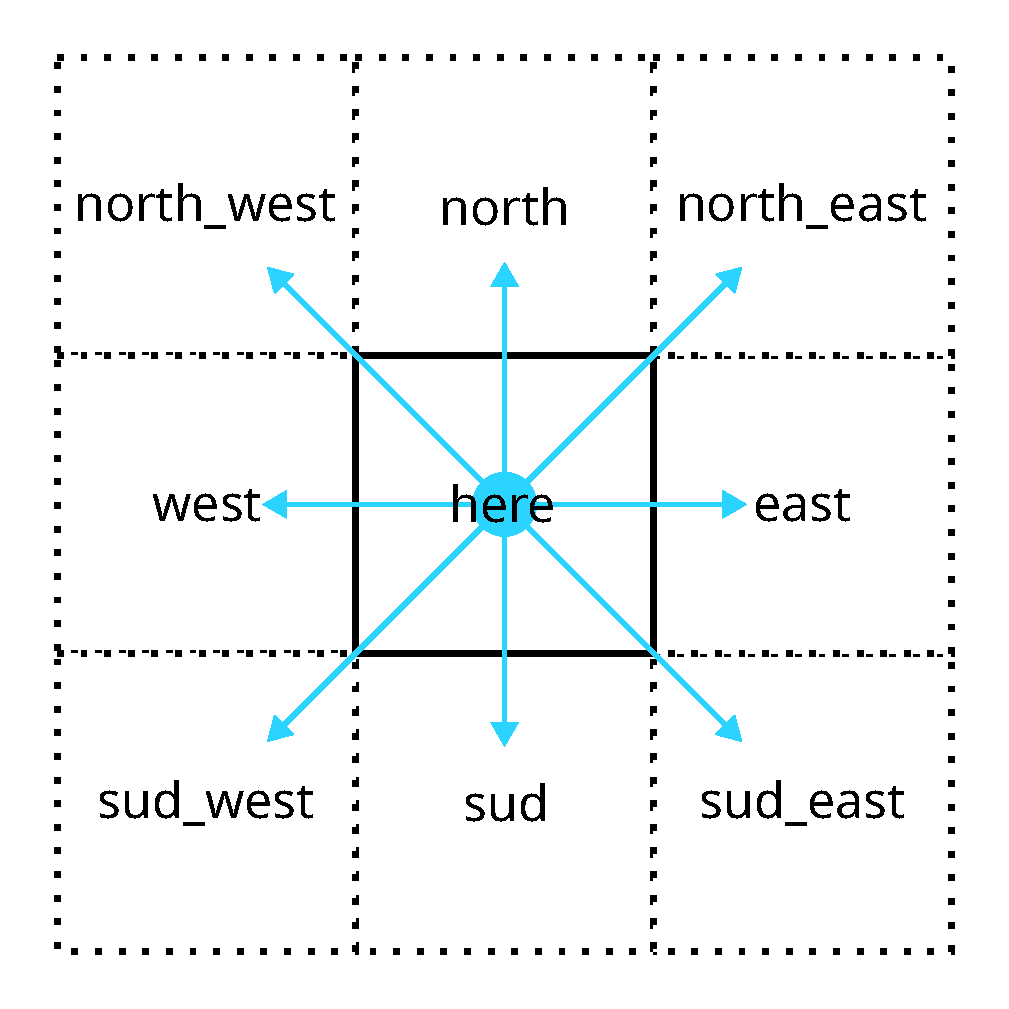
\includegraphics[width=.45\linewidth]{figures/ecai25/directions.pdf}
        \label{fig:directions}
    }
    \hfill
    \subfloat[Example of environment model]{
        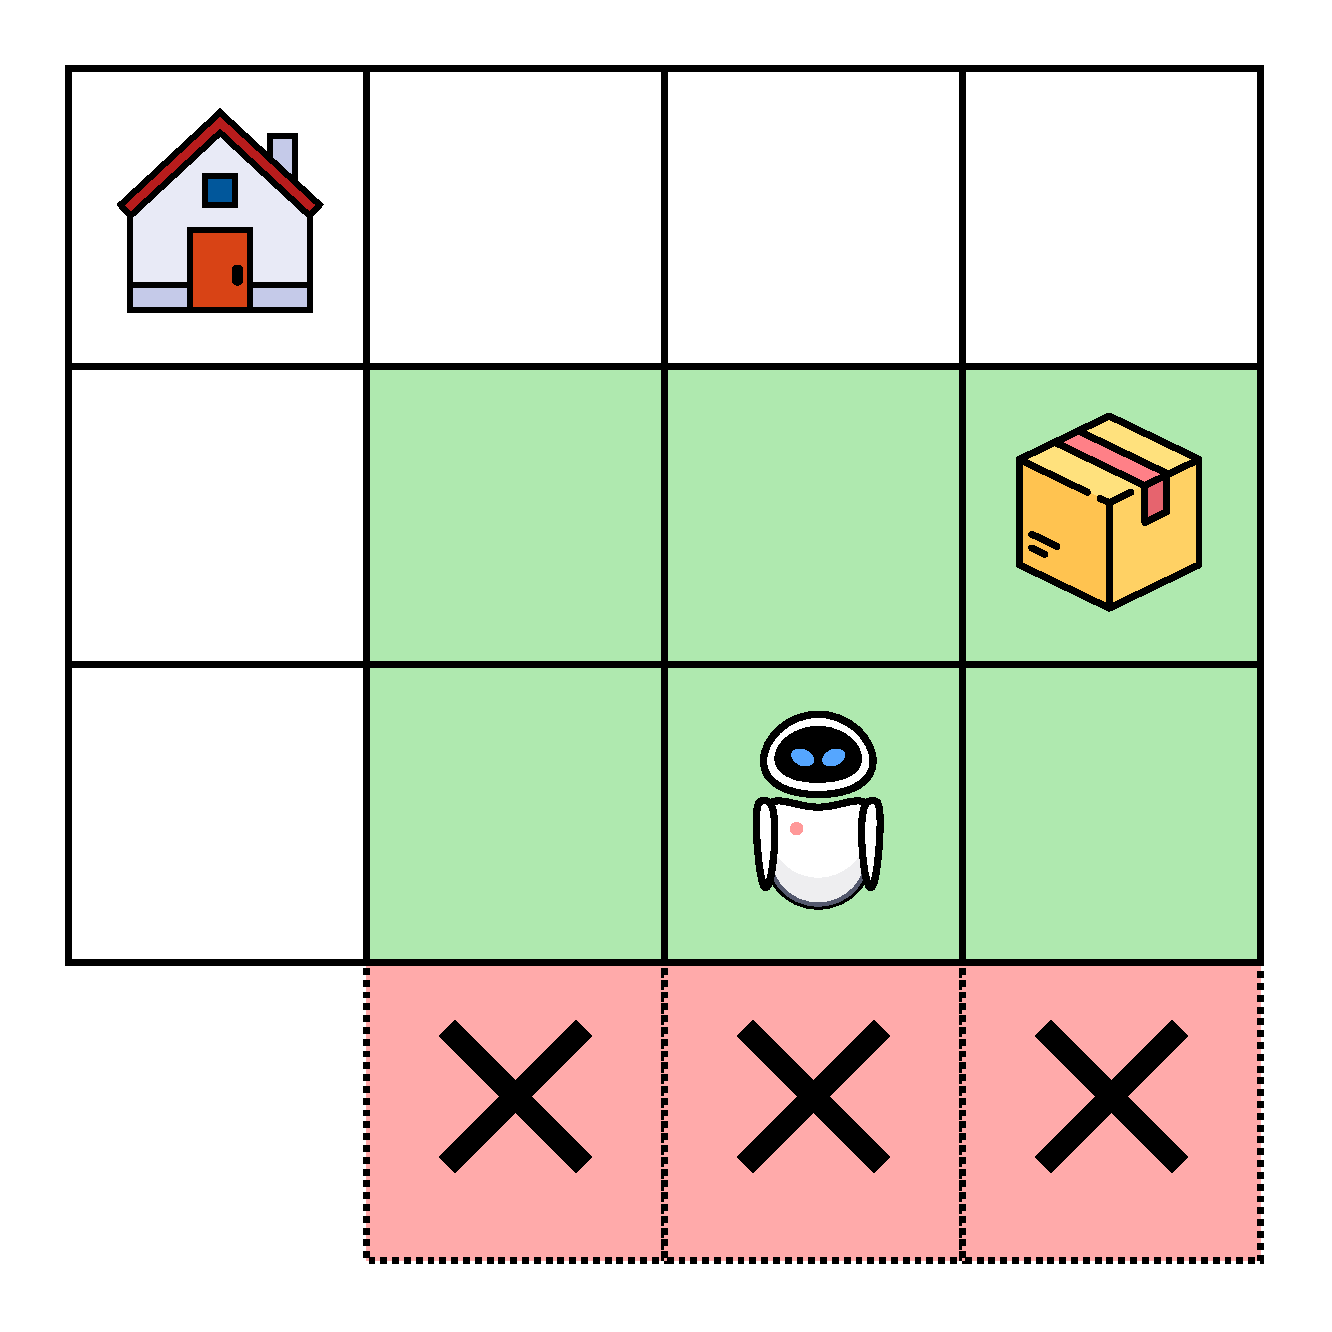
\includegraphics[width=.45\linewidth]{figures/ecai25/world.pdf}
        \label{fig:model}
    }
    
    \subfloat[Perceptions of the agent in \cref{fig:model}]{
        \makebox[0.5\linewidth][c] {
            \lstinputlisting[
                linewidth=0.4\linewidth,
            ]{figures/ecai25/perceptions.asl}
            \label{fig:perceptions}
        }
    }

\end{figure}

\paragraph{Example.}\label{sec:pgp-example}

% To clarify the concepts above,
% and the overall approach we are proposing,
From now on,
we rely on a running example.
%
Consider %for instance
the case of the \agentspeak{} agent depicted in \Cref{fig:environment-model}.
%
The agent is located in a grid 2D environment,
where it can move in 9 admissible directions
(i.e., the 8 cardinal directions plus \inlineAsl{here}, which implies no movement),
via the action \inlineAsl{move(Direction)},
unless there is an obstacle or a border in the way.
%
In any given moment,
the agent can perceive the environment,
expressed as in \Cref{fig:perceptions}.
%
% Particularly,
% it can perceive the presence of obstacles in the 8 cells surrounding it,
% via beliefs of the form \inlineAsl{obstacle(Dir)},
% which may be prefixed by $\neg$ to denote the absence of an obstacle
% in that \inlineAsl{Dir}ection.
%
% Similarly,
% the agent can perceive the presence of objects in its surroundings,
% via beliefs of the form \inlineAsl{there\_is(Obj, Dir)}.

Assuming that the agent is initially located into some cell where object \inlineAsl{home} is not even perceived,
and that it has the initial goal to \inlineAsl{reach(home)},
yet it has no plan to achieve this goal.
%
In such a situation,
the agent may trigger the \ac{PGP} to figure out what to do to handle goal \inlineAsl{!reach(home)}.
%
A good implementation of the \ac{PGP} would generate a set of plans $\mathcal{P} = \{p_1, p_2, p_3\}$ such as:
%
% \begin{lstlisting}[label={lst:pgp-result1}, caption={Example of generated plans}, captionpos=b]
\begin{lstlisting}
(*@$p_1$ $\equiv$@*) +!reach(Obj) : there_is(Obj, here).

(*@$p_2$ $\equiv$@*) +!reach(Obj) : there_is(Obj, Dir) <-
        move(Dir).

(*@$p_3$ $\equiv$@*) +!reach(Obj) : (*@$\neg$@*)there_is(Obj, _) <-
        ?random_free_dir(Dir); move(Dir); !reach(Obj).
\end{lstlisting}
%
which are actually good to \inlineAsl{reach} any object \inlineAsl{Obj}%
---not just \inlineAsl{home}.
%
There,
plan $p_1$ handles the success case where the object \inlineAsl{Obj} is already in the agent's current position,
then there is nothing to do,
as the initial goal has been already achieved.
%
Plan $p_2$ handles the case where the object is perceived in the surroundings of the agent,
in some \inlineAsl{Dir}ection:
the agent can now achieve the initial goal in one single \inlineAsl{move}ment.
%
Finally,
plan $p_3$ handles the case where the object is not perceived in the surroundings of the agent,
which means the agent has to explore the environment to find it.
%
The exploration is then attempted via a dummy strategy:
\emph{randomly} choosing a free \inlineAsl{Dir}ection,
then \inlineAsl{move}ing and recursively pursuing \inlineAsl{!reach(Obj)}.

From a technical perspective,
the \ac{PGP} generates a plan $p_1$ and $p_2$ by simply combining
goals, beliefs, and action names that are already known to the agent.
%
However,
in generating plan $p_3$,
the \ac{PGP} also \emph{invents} a new goal \inlineAsl{?random\_free\_dir(Dir)},
which is not known to the agent either at compile or run time.
%
Semantically,
this is a \emph{test} goal,
aimed at selecting one random obstacle-free direction,
yet,
technically,
this is a goal for which the agent has no plan.

Before executing plan $p_3$,
the agent may trigger the \ac{PGP} again,
to generate a plan for the subgoal \inlineAsl{?random\_free\_dir(Dir)}.
%
This time the \ac{PGP} may generate a plan $p_4$ such as:
%
\begin{lstlisting}
(*@$p_4$ $\equiv$@*) +?random_free_dir(Dir) : free(Dir) (*@$\wedge$@*) Dir(*@$\neq$@*)here.
\end{lstlisting}
%
Now the agent has all the plans it needs to achieve the initial goal \inlineAsl{!reach(home)},
so it can proceed executing them.

\subsection{When Should Plans Be Generated?}\label{sec:pgp-when}
In other words,
when should the agent trigger its \ac{PGP}?
%
Abstracting from technicalities,
and taking inspiration from prior literature on plan generation in \ac{BDI} agents,
we can identify two %three
main approaches to the triggering of \ac{PGP},
namely:
the reactive and the proactive ones. %, and on-demand approaches.
%
% Each approach comes with different assumptions and implications,
% concerning the role of the agents' programmer,
% the shape of the generated plans,
% and the autonomy of the agent.

\paragraph{On-demand \acs{PGP}.}

The on-demand \ac{PGP} is modelled as an \emph{action} that the agent can invoke whenever it needs to generate a plan.
%
Technically speaking,
the agent is assumed to have a built-in action \inlineAsl{generate\_plan(E)} in its action repertoire,
which it can invoke whenever it needs to generate a plan for event \inlineAsl{E}.
%
As an ordinary \agentspeak{} action,
\inlineAsl{generate\_plan} may appear in the body of any plan,
and be exploited by programmers to build smarter agents.
%
The action would just require the agent to provide some actual event \inlineAsl{E} as input,
and its effect would be the production of a plan of the form \inlineAsl{E <- C : \ldots},
where \inlineAsl{C} is the context of the plan,
to be added to the invoking agent's plan library.
%
Any failure in the \ac{PGP} execution results in a failure of the action,
handled by the agent as it would do for any other action.
%
The underlying assumption here is that
the programmer decides when the agent should trigger the \ac{PGP}.
%
% In fact,
% by writing ordinary \agentspeak{} plans,
% programmers may decide to exploit the \inlineAsl{generate\_plan} action to govern what exact plan should be generated,
% and under which conditions.
% %
% Another consequence of this approach is that,
% by looking at an agent's plan library,
% one may easily identify which and how many goals are going to require plan generation.
% %
% This may be useful for debugging purposes,
% or to understand the agent's behaviour in advance.

% It is worth noticing that,
As a consequence of constraint \ref{item:allowed-refs},
the \ac{PGP} may generate plans that use the \inlineAsl{generate\_plan} action in their body.
%
So, generated plans may themselves trigger the \ac{PGP} to generate new plans, when executed.
%
This powerful feature allows the agent to hierarchically generate plans,
possibly decomposing complex plans into simpler ones,
and so on recursively%
---provided that
the underlying \ac{LLM} is smart enough to understand when it is wise to postpone the generation of a (sub-)plan,
and when it is better to generate it immediately.

\paragraph{Reactive \acs{PGP}.}

The reactive \ac{PGP} is implicitly triggered by the agent's control loop
whenever an event \inlineAsl{E} occurs and the agent has no applicable plan for it.
%
So,
an unknown event
would trigger the \ac{PGP} instead of making the current intention fail.
%
If the \ac{PGP} fails, 
the current intention fails as when there is no plan were available;
if it succeeds,
the agent proceeds as if the plan existed from the start.

% The reactive approach could be considered as a refinement of the on-demand one,
% where the \ac{PGP} is automatically triggered by the agent's control loop,
% rather than explicitly invoked by the agent's programmer.
% %
% In fact,
Provided that agents are equipped with the aforementioned \inlineAsl{generate\_plan} action,
one may consider implementing the reactive approach as shown below: %in \Cref{lst:recative-pgp}:
%
% \begin{lstlisting}[label={lst:recative-pgp}, caption={One possible implementation of a reactive \ac{PGP}}, captionpos=b]
\begin{lstlisting}
(*@$p_\mathit{genex}$ $\equiv$@*) -G : missing_plan_for(G) <- generate_plan(G); G.
\end{lstlisting}
%
There,
we borrow \jason{}'s extended \agentspeak{} syntax (cf. \cite{BordiniHW2007}) for failure handling plans %\footnotemark{}
to express a plan (namely, $p_{genex}$) reacting to the failure event provoked by the absence of a plan for goal \inlineAsl{G},
to which the agent should react by generating a plan for it,
and finally pursue goal \inlineAsl{G} one more time.
%
The underlying assumption here is that agents are equipped by default with plan $p_\mathit{genex}$,
as well as with a special belief \inlineAsl{missing\_plan\_for(G)},
which computes whether plans are missing in the agent's plan library for goal \inlineAsl{G}.
%
% \footnotetext{
%     \jason{} is an implementation of \agentspeak{} which extends the syntax in many ways,
%     there including failure events of the form \inlineAsl{-G},
%     which occur when some plan for goal \inlineAsl{G} fails or none is available.
% }

The reactive approach improves the on-demand approach by making the generation procedure automatic,
and therefore implicit.
%
Neither the programmer nor the \ac{LLM} generating plans needs to explicitly trigger the \ac{PGP}:
the agent will handle this automatically
when it encounters a goal without an associated plan during execution.
%
% In fact,
% another benefit here is minimality \ac{PGP} of executions:
% aside from explicit invocations,
% the \ac{PGP} is triggered only when strictly necessary.

% Finally,
The reactive approach as well supports the generation of hierarchies of plans,
in a way which is similar to the example from \Cref{sec:pgp-example}.
%
% In fact,
% as prescribed by constraint \ref{item:novel-refs},
% the \ac{PGP} may generate plans that refer to novel, unknown goals.
% %
% When met at run-time,
% the agent will trigger the \ac{PGP} again to generate a plan for the new goal,
% and so on recursively.
%
The main difference here is that the \ac{LLM} is not required
to be aware of the recursive nature of the planning activity it is involved into.
%
So,
it can focus on the problem suggesting the best subgoals and actions to be performed to pursue a given goal.

% \paragraph{Proactive \acs{PGP}.}

% In the proactive approach,
% the \ac{PGP} is triggered by an ad-hoc, background intention,
% which is assumed to be built-in in each agent.
% %
% The intention would be responsible for continuously monitoring the agent's internal state,
% looking for goals or events for which the agent has no plan,
% and triggering the \ac{PGP} for each of them.
% %
% In case that no plans are missing,
% the intention would simply suspend itself or do nothing,
% waiting for further plans or goals being added to the agent%
% ---as these may contain new goals or events which require plan generation.

% Conceptually speaking,
% such an intention is never meant to terminate.
% %
% Rather,
% it should carry on the following operations in a loop:
% %
% \begin{inlinelist}
%     \item select one event \inlineAsl{E} for which no plan is available in the agent's plan library;
%     \item trigger the \ac{PGP} to generate a plan for \inlineAsl{E} on a new intention
%     -- so to allow multiple, concurrent \acp{PGP} for different events --
%     % \item wait for the addition of plans or goals in the agent's internal state;
%     \item repeat.
% \end{inlinelist}
% %
% Borrowing again from \jason{} syntax,
% we can express the proactive approach as follows:
% %
% \begin{lstlisting}
% (*@$g_\mathit{init\ }$ $\equiv$@*) !generate_plans.

% (*@$p_\mathit{scan}$ $\equiv$@*) !generate_plans <-
%         for (event(E) & missing_plan_for(E)) {
%             !!pgp(E)
%         }; !generate_plans.

% (*@$p_\mathit{gen\ }$ $\equiv$@*) !pgp(E) <- generate_plan(E).
% \end{lstlisting}
% %
% There,
% gaol $g_\mathit{init}$ is one built-in initial goal of the agent,
% whose only purpose is to start the generation intention along with the agent.
% %
% Plan $p_\mathit{scan}$ is a scanning plan:
% it selects known events from the agent's internal state
% -- via the special belief \inlineAsl{event(E)}, plus the aforementioned \inlineAsl{missing\_plan\_for} one --
% and triggers plan $p_\mathit{gen}$ on a new intention for each of them.
% %
% Plan $p_\mathit{gen}$,
% in turn,
% triggers the \ac{PGP} to generate a plan for the event \inlineAsl{E},
% without executing it thereafter.
% %
% Any failure in plan $p_\mathit{gen}$ would not interrupt plan $p_\mathit{scan}$,
% as it is running on a different intention.

% Similarly to the reactive approach,
% the proactive one allows for the generation of hierarchical plans,
% without requiring any explicit action by either the agent's programmer or the \ac{LLM}.
% %
% Yet,
% by anticipating the \ac{PGP} execution,
% it may also mitigate the risk of the agent being stuck waiting for the \ac{PGP} to terminate,
% while also being in \emph{urgent} need of a plan to know how to act.
% %
% The drawback however is that race conditions may occur,
% for instance between an intention needing some missing plan,
% and the intention in charge of generating it.
% %
% So,
% it may happen that one intention fails out of a missing plan,
% because the intention in charge of generating it has not been executed yet.
% %
% This is a problem that may be solved by the agent's programmer,
% at the expense of additional coding efforts.

\subsection{Concurrency and \ac{PGP}}

Regardless of how/when the \ac{PGP} is triggered,
any implementation approach should consider that the \ac{PGP} is inherently \emph{blocking} for the agent.
%
In fact,
at the current state of technology,
\acp{LLM} are commonly queried via Web services (contacted over the Internet),
and they may take up to many seconds to complete their response
(or even fail, e.g. due to network issues).
%
Even by assuming that the \ac{BDI} agent and the \ac{LLM} are running on the same machine,
the \ac{LLM} may require entire seconds to generate a plan.
%
Large time scales may be unacceptable for \ac{BDI} agents,
especially if waiting for the \ac{PGP} to terminate implies blocking the agent's control loop.
%
This would hinder the agents' ability to react to events in a timely manner,
and therefore its autonomy.

To mitigate this problem,
implementers should consider \emph{suspending} only the intention that triggered the \ac{PGP},
rather than the whole control loop of the agent.
%
As multiple intentions may be concurrently carried on by an \agentspeak{} agent,
this would allow it to ``keep thinking about how to react to event \inlineAsl{E},
while doing something else''.

% \subsection{Evaluating and Revising Plans}

% \gcnote{
%     We should discuss what mechanisms could be put in place for the agent to be able to automatically assess whether a generate plan is good or not.
%     Then there's the problem of revising plans, which is a bit more complex.
%     It is very much likely that this section will just become a future work.
% }
% \ganote{
%     Yes I agree to move this to future work. We should focus on what we already have.
% }

\section{Transferring Knowledge between \ac{BDI} agents and \acp{LLM}}\label{sec:remarks}

Here we delve into the practical aspects of endowing \ac{BDI} agents with a \ac{PGP},
we discuss
how to effectively engineer the prompts for \ac{LLM} to let it generate plans,
and
how to write agent specifications in \agentspeak{},
to enrich them with additional knowledge that can be exploited by the
new generative capabilities.

\subsection{From \acs{BDI} Agents to \acp{LLM} and Back}

% \gcnote{
%     TODO: discuss how prompts are engineered in order for \ac{LLM} to generate plans.
%     Aspects to be discussed:
%     1. what to encode (believes, goals, plans, available actions, etc.);
%     2. what contextual information to provide to the \ac{LLM} aside from the above;
%     3. how to encode agent information to be sent to the \ac{LLM} (natural language, \agentspeak{} code, Prolog code, etc.) in order to get parsable output;
%     4. how to parse the output to bring it back into \agentspeak{};
% }
In practice, how should the \ac{PGP} operate to work as discussed so far?

Technically, when triggered for a goal \inlineAsl{G}, the \ac{PGP} should:
%
\begin{inlinelist}
    \item convert the agent's internal state, as well as \inlineAsl{G}, into the textual prompt used to query the \ac{LLM} of choice,
    then
    \item parse the \ac{LLM} response to extract the generated plans.
\end{inlinelist}
%
The specific \ac{LLM} chosen does not impact the design of the \ac{PGP} itself,
yet it may affect the quality of the generated plans---as we further discuss in \Cref{sec:experiments}.

So, \emph{prompt generation} (structured information into free text)
and  \emph{parsing} (free text back into structured information)
are the two main \emph{complementary} activities of \ac{PGP}.
%
They may be implemented in several ways,
mostly differing in terms of \emph{what to encode}, and \emph{how to encode} it,
in the \ac{LLM} prompt and in the response.

\subsubsection{What to Encode}\label{sec:pgp-encoding}

% For the sake of clarity, in the following
% we describe the \ac{PGP} backwards, from its end back to its start.
% to better understand the rationale behind our proposed encoding.

\paragraph{The Response.}
%
The \ac{PGP} should produce a set of \ac{BDI} plans by querying some \ac{LLM},
which in turn produces a textual response.
%
The response represents a (possibly empty) collection of plans,
where each plan should involve:
%
\begin{inlinelist}
    \item a triggering event,
    \item a context -- i.e., a (possibly empty) collection of conditions to test --,
    and
    \item a body---i.e. a (possibly empty) collection of subgoals and actions.
\end{inlinelist}

\paragraph{The Prompt.}
%
To support the aforementioned plans generation,
the \ac{PGP} should provide all
(and possibly only)
relevant information to the \ac{LLM}
via some \emph{automatically}-generated prompt,
following a typical zero-shot prompting approach~\cite{KojimaGRMI22},
therefore encoding instructions and information about the
agent's current state in natural language and in structured form,
thus addressing \ref{rq:required-info}.
%This directly addresses \ref{rq:required-info} (what information LLMs require).

Conceptually speaking,
relevant information should include:
%
\begin{enumerate*}[label=\textbf{(I\arabic*)}]
    \item\label{item:goal} the intended meaning of the goal \inlineAsl{G} for which the plans are needed
    -- plus the explicit request to generate plans for it --,
    \item\label{item:admissible} goals, actions, and beliefs known to the agent,
    \item\label{item:current} the agent's currently handled plans, goals, and beliefs;
    as well as instructions on
    \item\label{item:pgp} what is the intended outcome of the plan generation process,
    \item\label{item:lang} the \agentspeak{} syntax and meaning,
    \item\label{item:task} how to impersonate a \ac{BDI} agent willing to generate a plan
    (i.e., role-playing prompting~\cite{KongZCLQSSZ23}),
    and
    \item\label{item:bdi} what a \ac{BDI} agent is in the first place.
\end{enumerate*}

%\gcnote{@Gianlu giù faccio sicuramente riferimento a qualche buona pratica di prompt engineering. Se ti vengono in mente citazioni aggiungile pure.}

Whereas the \ac{LLM} needs \ref{item:goal} to know what goal the agent is willing to pursue
-- in our running example, the goal \inlineAsl{!reach(home)} --
\ref{item:admissible} is required to know which goals, actions, or beliefs (akin to tool specifications in ReAct~\cite{YaoZYDSN023})
the \ac{LLM} could use to generate the plans.
%
For instance,
some generated plans may check for obstacles in the surroundings of the agent via belief \inlineAsl{obstacle(Dir)},
even if the agent is currently not perceiving any obstacle.
%
%The explanation of action \inlineAsl{move(Dir)} would fit here too,
%as well as a general descriptions of goals of the form \inlineAsl{!reach(Obj)}.

For the \ac{LLM} to account for the context currently perceived by the agent when generating the plans, \ref{item:current} is needed.
%
For instance, beliefs such as \inlineAsl{there\_is(box, north\_east)} and \inlineAsl{obstacle(north)} should be included here.
%
\ref{item:pgp} informs the \ac{LLM} about the purpose and the constraints of the plan generation process,
as defined in \Cref{sec:pgp}.
%
This is where,
for instance,
the possibility to formulate new goals and beliefs should be mentioned---%
along with the impossibility of creating new actions.

\ref{item:lang} lets the \ac{LLM} comply with the \agentspeak{} syntax,
when both reading the prompt and producing its response,
and makes it aware of how cognitive abstractions are modelled in \agentspeak{}.
%
This is where,
for instance,
the \ac{LLM} is informed about the three parts of a plan (event, context, and body),
and the components of a plan body (subgoals and actions).
%
Along with \ref{item:bdi},
-- where the general notions of beliefs, desires, and intentions are provided --
the core idea here is to provide the \ac{LLM} with enough background knowledge to operate in the \ac{BDI} domain,
regardless of whether \ac{BDI} literature has been included in the training set of the \ac{LLM} or not.

Finally,
\ref{item:task} provide the \ac{LLM} with meta-level suggestions about how to devise plans in general.
%
There, recommendations such as ``decompose the task hierarchically''
or ``re-use the known goals and actions whenever useful'' could be included.

It is worth noticing that,
while \ref{item:goal}, \ref{item:admissible}, and \ref{item:current} are specific to the agent's current state,
\ref{item:pgp}, \ref{item:lang}, \ref{item:task}, and \ref{item:bdi} are more general,
and could be factoreised across different runs of the \ac{PGP}.

\subsubsection{How to Encode~\ref{rq:knowledge-transfer}}
In principle flexibility in syntax is allowed for both the prompt and the response,
provided that
%
\begin{inlinelist}
    \item\label{syntax:prompt} the syntax used for the prompt is easily manipulable by the \ac{LLM},
    \item\label{syntax:response} the syntax used for the response is easily parsable by some non-\ac{LLM}-based parser.
\end{inlinelist}
%
A complete example of a prompt satisfying our recommendations is provided
in the supplementary materials~\cite{ZenodoSupplementaryMaterial}.
%
% Here we briefly summarise its main features.

To achieve \ref{syntax:prompt},
we recommend maximizing the exploitation of natural language (as done in related works in LLM as a ``planner''~\cite{Murugesan25a})---
which does not mean discarding \agentspeak{} syntax,
but rather complementing it with natural language descriptions.
%
For instance, when describing the goal \inlineAsl{!reach(Obj)} in the prompt,
a natural language description like
``the agent wants to reach a situation where \inlineAsl{Obj} is perceived in its surroundings''.
%
Similarly,
the admissible belief \inlineAsl{there\_is(Obj, Dir)} could be described as
``the agent can perceive the presence of \inlineAsl{Obj} in direction \inlineAsl{Dir}''.
%
Likewise, this applies to every admissible/current goal, belief, or action.

To achieve feature \ref{syntax:response},
we recommend using a syntax that is as structured as possible,
where the boundary between one generated plan and the next one is easily identifiable,
and each section of the plan
(event, context, operations)
is clearly delimited.
%
This could be achieved by using the \agentspeak{} syntax directly,
or,
if the \ac{LLM} is not good at it
(likely to happen for small \acp{LLM})
by using a more famous syntax,
such as Prolog or YAML.
%
So,
for instance,
one may ask the \ac{LLM} to generate plans matching the following template:
%
\begin{lstlisting}
EVENT:
  (*@$\mathit{verb}$@*): event
CONDITIONS:
  - condition
  - other_conditon
  - ...
OPERATIONS:
  - (*@$\mathit{verb}$@*): operation1
  - (*@$\mathit{verb}$@*): operation2
  - ...
\end{lstlisting}
%
where $\mathit{verb}$ is a keyword among \inlineAsl{execute}, \inlineAsl{achieve}, \inlineAsl{test}, \inlineAsl{add}, \inlineAsl{remove}, and \inlineAsl{update}.
%
This format can be parsed by programming languages, 
is human-readable and debuggable, 
and can be generated by the \ac{LLM}, 
as it aligns with well-known syntaxes (e.g., YAML).

It is worth mentioning that
a description of the expected response syntax should be included in the prompt
to let the \ac{LLM} know what is expected from it.
%
This is acknowledged as the most common way to control the shape of the \ac{LLM} response,
and it is commonly referred to as \emph{structured output}~\cite{TangZPZCG23}.
%
In our perspective,
the ``structured output instructions'' are yet another information to be included in the prompt,
along with the other items discussed above.

\subsection{Writing Generative Agent Specifications}\label{sec:writing}

% \gcnote{
%     TODO: discuss here how the role of \ac{BDI} agents changes when agents are generative.
%     Insight: less code to be written, yet some code should be written to inform the agent on how to generate the missing plans.
%     The agent-oriented programming language should be evolved too, to support new syntactical categories, aimed at letting programmers specify hints for plans generation.
%     Let's provide examples which are directly tailored on \jakta{}, to save space.
% }

When \ac{BDI} agents are generative and can generate their own plans,
one may wonder how the role of the programmer changes, to account for such new capabilities.
%
In other words, do agents still need programmers to write their plans?
%
Given the current state of technology,
we argue that %the answer is `yes, but less':
programmers are still needed to write the initial plans of the agent,
and they are also required to provide hints about the intended semantics of the goals, beliefs, and actions they write.
%
The latter point in particular (writing hints) is the main focus of this section.
Namely, we aim to show how developers can provide additional domain knowledge to the \ac{LLM} in an easily maintainable way, alongside the agent's specification, addressing \ref{rq:agent-spec}.
This focuses on transferring knowledge to the \ac{LLM} to improve plan generation.

In the general case,
it is not guaranteed that \acp{LLM} will be able to understand the intended meaning of the goals, beliefs, and actions
they are asked to generate plans for/with.
%
This is because there is no guarantee that \ac{BDI} programmers would use intuitive and self-explanatory names for them,
or, that the \ac{LLM} is trained on the \ac{BDI} programming language of choice.
%
For this reason,
we designed the encoding procedure (cf. \Cref{sec:pgp-encoding}) to include some natural-language
description of each aspect of the agent's internal state.

Yet,
descriptions cannot be automatically generated
-- as automatic procedures may be inaccurate or incomplete w.r.t.\ the programmer's intent --
so programmers need to write them directly.
%
Descriptions should be written in natural language and explain the meaning of
the \emph{admissible} and \emph{actual} goals, beliefs, and actions each agent has.

Accordingly,
our \ac{PGP}-equipped \ac{BDI} agent requires one final assumption:
agent programs should be written in a way that
\begin{inlinelist}
    \item natural-language descriptions for admissible and actual mental abstractions are part of the agent's code,
    and
    \item those descriptions are used to generate the prompt for the \ac{PGP}.
\end{inlinelist}
%
To this end,
the \agentspeak{} framework, and consequently \ac{BDI} programming languages, should be extended with ad-hoc syntactical constructs for
tagging cognitive abstractions with their intended meaning.
%
Furthermore,
to minimize the programmer's burden,
these constructs should be optional,
and allow for templating and reusing descriptions.

Consider for instance the \inlineAsl{obstacle(Dir)} beliefs in \Cref{fig:perceptions}.
%
When generating an \ac{LLM} prompt for them,
the \ac{PGP} should
\begin{inlinelist}
    \item describe the general meaning beliefs of the form \inlineAsl{obstacle(Dir)}
    -- namely: ``an obstacle is perceived in direction \inlineAsl{Dir}'' --
    and
    \item describe the specific meaning of each belief of this sort that the agent currently has%
    % also considering that it may or may not be negated%
    ---namely: ``there is an obstacle in direction north''.
\end{inlinelist}
%
Yet,
there is no need for the programmer to write all these descriptions by hand,
as they can be automatically generated out of templates.

We prototype these ideas in \jakta{}~\cite{DBLP:journals/sncs/BaiardiBCP24},
an \agentspeak{}-based programming language
implemented as a Kotlin \ac{DSL}%
---therefore easily extensible with additional syntactical constructs.
%
In \jakta{},
% the code of the agent from \Cref{fig:environment-model} would be look like the one in \Cref{lst:jakta-code}.
% %
% \lstinputlisting[
%     float,
%     label={lst:jakta-code},
%     caption={Example of a \jakta{} agent extended with natural-language descriptions},
%     language=Kotlin,
%     basicstyle=\tiny\ttfamily
% ]{listings/jakta-code.kt}
% %
% There,
the new entries are (cf. Section C in \cite{ZenodoSupplementaryMaterial}):
\begin{inlinelist}
    \item the \texttt{.meaning\{\ldots\}} blocks,
    which can be used to tag \emph{actual} goals, beliefs, or actions with their intended meaning,
    via a post-fix syntax;
    and the
    \item the \texttt{admissible\{\ldots\}} blocks,
    which can be used to tag \emph{admissible} goals or beliefs with their intended meaning,
    via a pre-fix syntax.
\end{inlinelist}
%
In both cases,
the meaning is expressed as a string,
attained via string interpolation,
which in turn may include the functor, the arguments, and the presence/absence of negation
of the tagged goal, belief, or action.
%
The strings are then exploited by the \ac{PGP} to generate the prompt for the \ac{LLM}.

\section{Experimental Evaluation}\label{sec:experiments}

Here we assess our approach empirically,
by evaluating the performance of the \ac{PGP} in generating plans for \ac{BDI} agents,
by indirectly assessing the quality of the generated plans.

\paragraph{Experimental Setup}

We implement the reactive \ac{PGP} approach as described in \Cref{sec:pgp} in a \jakta{} agent~\cite{DBLP:journals/sncs/BaiardiBCP24},
whose specification is enriched with natural-language descriptions as discussed in \Cref{sec:writing}.
%
The experiment is publicly available\footnote{github.com/pslab-unibo/experiment-2025-ECAI-generative-bdi-agents} 
and archived on Zenodo~\cite{ZenodoArtifact}.
%
The agent has to reach home within a simulated 2D grid world environment
where it can perceive obstacles, with no pre-programmed knowledge.
%
The setup mirrors our running example throughout the chapter.
%
We conduct the experiment across multiple popular and publicly available LLM models
(specifically: \texttt{gpt-4.1}, \texttt{gemini pro 2.5}, \texttt{deepseek V3}, and \texttt{claude 3.7 thinking}),
iterating each experiment $5$ times per model
to account for the stochastic nature of LLM responses,
resulting in a total of 20 experimental runs.

\paragraph{Metrics}
To assess the quality of generated plans
we combine automatic and manual evaluation procedures,
as our goal is to assess hard properties of the generated plans
(e.g., syntactical correctness or functionality, which can be automatically tested),
but also soft properties (e.g., relevance, usefulness, readability, etc.) 
which are hard to formalize and automatically infer.
%
To evaluate the quality of generated plans, we define the following metrics:
\newcommand{\PC}{\textbf{PC}}
\newcommand{\CC}{\textbf{CC}}
\newcommand{\PBC}{\textbf{PBC}}
\newcommand{\GR}{\textbf{GC}}
\newcommand{\RA}{\textbf{RA}}
\newcommand{\NGC}{\textbf{NGC}}
\newcommand{\NBC}{\textbf{NBC}}
\newcommand{\GSM}{\textbf{GSM}}
\newcommand{\BSM}{\textbf{BSM}}
\newcommand{\TSR}{\textbf{TSR}}
\newcommand{\GAT}{\textbf{GAT}}
\newcommand{\PRAS}{\textbf{PRAS}}
\begin{itemize}
    \item \emph{Plan Count} (\PC): Total number of generated plans.
    \item \emph{Context Complexity} (\CC): Average number of beliefs per plan context.
    \item \emph{Plan Body Complexity} (\PBC): Average number of operations per plan body.
    \item \emph{Generalization Count} (\GR): Number of generated plans that use variables (general) rather than constants (specific).
     \item \emph{Redundancy Amount} (\RA): Amount of generated plans which are useless (e.g., not executable at runtime or subsumed by more general plans).
    \item \emph{Novel Goal Count} (\NGC): Number of newly-invented goals.
    \item \emph{Novel Belief Count} (\NBC): Number of newly-invented beliefs.
    \item \emph{Goal Semantic Misalignment} (\GSM): Number of semantically-misaligned uses of admissible goals.
    \item \emph{Belief Semantic Misalignment} (\BSM): Number of semantically-misaligned uses of admissible beliefs.
    \item \emph{Task Success Rate} (\TSR): Percentage of experiments where the agent successfully achieves the \inlineAsl{!reach(home)} goal.
    %\item \emph{Goal Achievement Time} (\GAT): Average time steps required to achieve the goal in successful experiments.
\end{itemize}
Among these metrics,
\GR{} and \TSR{} should be maximised (higher values are better),
while \RA{}, \GSM{}, \BSM{}, should be minimised (lower values are better).
%
The remaining metrics (\PC{}, \CC{}, \PBC{}, \NGC{}, and \NBC{}) have no clear optimization direction,
yet they provide valuable comparative insights, with both extremely low and high values potentially indicating issues.

Additionally,
to establish a comprehensive evaluation metric for plan quality,
we implement a \textbf{Plan-Reference Alignment Score (\PRAS{})} comparing generated plans against expert-designed reference plans.
%
For this purpose,
we exploit an LLM explicitly as a judge~\cite{DBLP:journals/corr/abs-2412-05579},
tasked with evaluating the quality of abstraction, generalizability,
and adherence to BDI principles in the generated plans compared to reference implementations---see Section D in \cite{ZenodoSupplementaryMaterial}.
%
This LLM-as-judge methodology allows us to systematically rate plan quality using criteria that
would be difficult to formalise through traditional metrics alone.
%
\PRAS{} tends to 1 when the generated plans are similar to the reference ones,
to 0 when they are completely different.

\paragraph{Results}
\Cref{tab:experiments} and \cite{ZenodoSupplementaryMaterial} (Section E) summarise the results of our experiments across different LLM models in terms of the defined metrics,
whereas \Cref{fig:pras} provides a visual representation of the \PRAS{} scores for each model.
%
In \cite{ZenodoSupplementaryMaterial} (Section B) we provide an example of a generated plan.
\begin{table}[t]
    \centering
        \caption{Experimental results across different LLM models. These number are averaged over 5 runs per model.}
        \label{tab:experiments}
        \footnotesize
        \begin{tabular}{@{}l@{\;}|r@{\;}r@{\;}r@{\;}r@{\;}r@{\;}r@{\;}r@{\;}r@{\;}r@{\;}|r@{\;}r@{\;}}
            \toprule
             \textbf{Model} & \PC{} & \CC{} & \PBC{} & \GR{} $\uparrow$ & \RA{} $\downarrow$ & \NGC{} & \NBC{} & \GSM{} $\downarrow$ & \BSM{} $\downarrow$ & \TSR{} $\uparrow$\\  \midrule
            Claude & 4.80 & 1.86 & 1.59 & 2.80 & 0.00 & 0.80 & 0.20 & 0.00 & 0.00 & 60\% & \\
            Deepseek & 5.00 & 1.52 & 1.96 & 1.00 & 0.40 & 1.20 & 1.60 & 0.20 & 1.00 & 40\% &  \\
            GPT 4 & 2.00 & 1.90 & 1.50 & 2.00 & 0.00 & 1.00 & 0.00 & 1.00 & 0.00 & 100\% \\
            Gemini Pro & 3.80 & 2.00 & 1.71 & 3.80 & 0.00 & 0.20 & 0.80 & 0.00 & 0.00 & 20\% \\
            \midrule
            Optimal & 3.00 & 1.00 & 1.30 & 3.00 & 0.00 & 0.00 & 0.00 & 0.00 & 0.00 & 100\% \\
            \bottomrule
        \end{tabular}
\end{table}
\begin{figure}[t]
    \centering
    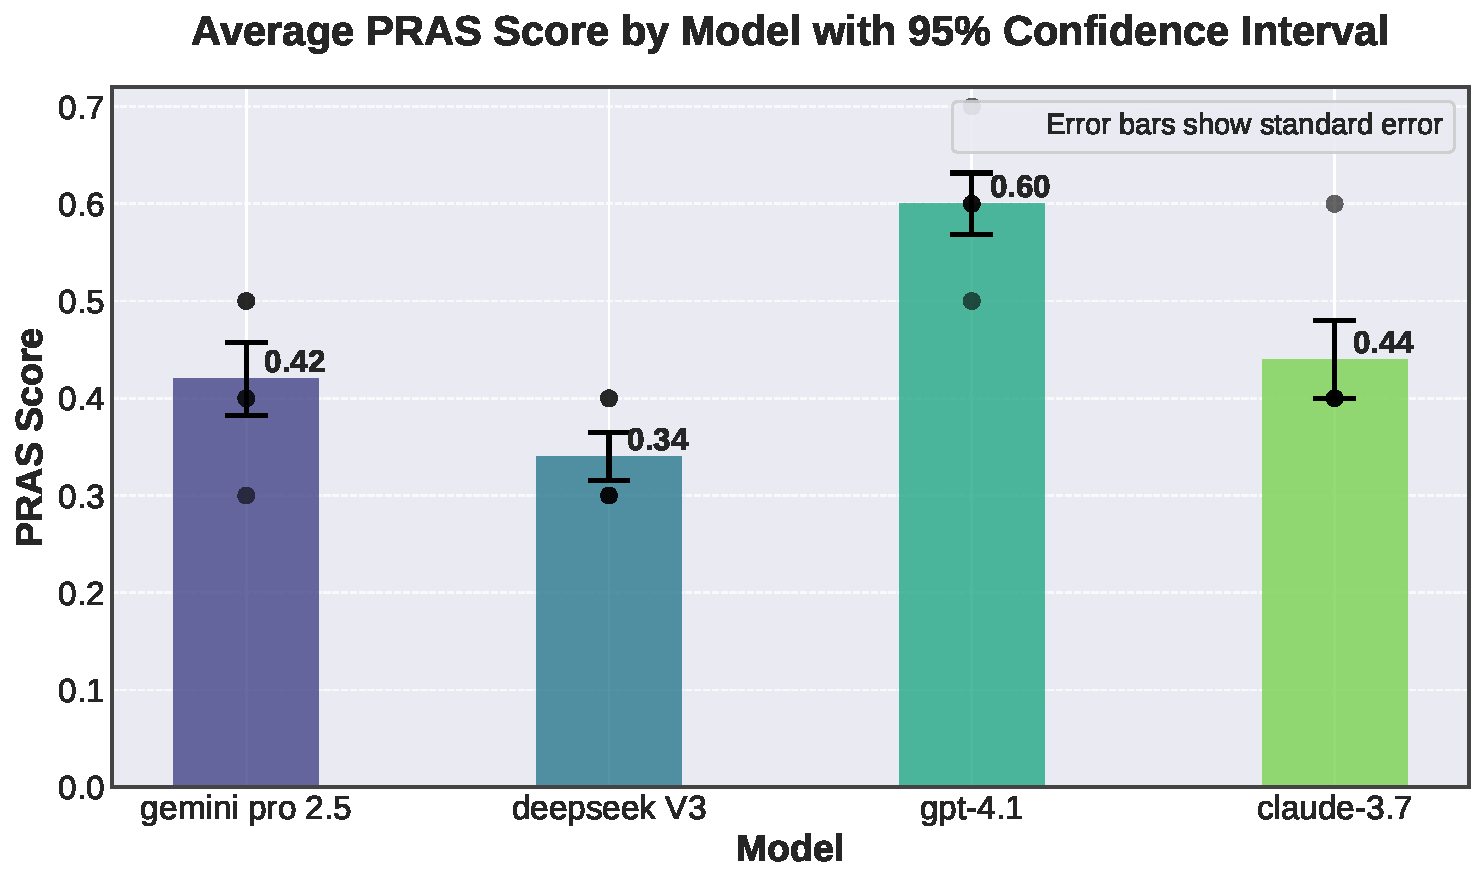
\includegraphics[width=0.8\columnwidth]{figures/ecai25/geval_results_bar_plot.pdf}
    \caption{\PRAS{} across different LLM models.}
    \label{fig:pras}
    \vspace{0.5cm}
\end{figure}
Task Success Rate (\TSR{}),
 our primary effectiveness indicator,
 varied considerably across models (Table 1).
%
GPT-4 demonstrated perfect performance with 100\% \TSR{}, producing consistently usable plans
 that successfully completed the task in all experimental runs,
 thereby matching the optimal baseline.
Claude achieved moderate success (60\% \TSR{}),
 while Deepseek (40\%) and Gemini Pro (20\%) struggled with task completion.

Another key indicator of plan quality,
 namely the \PRAS{} score,
 indicated that GPT-4 generated plans most closely resembling expert-designed reference plans (0.60),
 suggesting a high degree of reusability (also due to its high \TSR{}).
%
Conversely, the other models exhibited lower \PRAS{} scores ($<0.50$),
 which may indicate a divergence from reference implementations.
These lower scores suggest differences in plan structure
 and strategy compared to expert-designed solutions,
 potentially reflecting model-specific reasoning patterns or
 limitations in interpreting the semantic constraints of the BDI architecture.
%
Despite generally positive alignment scores,
plans generated by most \acp{LLM} diverged significantly from
the baseline in terms of structure and complexity,
as evident from the results.
%
Complexity analysis showed that \acp{LLM} generally produced more elaborate solutions than the optimal baseline (\PC{}=3.00, \CC{}=1.00, \PBC{}=1.30).
%
Most models generated higher plan counts (Deepseek: 5.00, Claude: 4.80),
context complexity (Gemini Pro highest at 2.00),
and plan body complexity (Deepseek highest at 1.96),
showing a tendency toward richer conditions and longer plans,
than the minimal optimal strategy.

Interestingly, however, Gemini Pro displayed the highest Generalization Count (3.80)
 among LLMs,
 surpassing even the optimal \GR{} (3.00),
 indicating a tendency to create abstract,
 variable-using plans.
%
However, this high generalization did not translate into effectiveness,
 given its low \TSR{}.
Conversely, Deepseek showed a significant Redundancy Amount (0.40),
 likely lowering its \TSR{}, while GPT-4 and Claude produced no redundant plans (\RA{} = 0.00).

For cognitive construct invention,
 Deepseek was most prolific (\NGC{} = 1.20, \NBC{} = 1.60),
 followed by GPT-4 (\NGC{} = 1.00, \NBC{} = 0),
 while Claude and Gemini Pro showed minimal invention.
%
This highlights LLMs' abstraction capabilities, though it can lead to unnecessary complexity, as seen in Deepseek's redundant plans.

Finally, the semantic alignment metrics assess
 the correct usage of pre-defined admissible goals and beliefs,
 leveraging the provided natural language descriptions.
%
Lower scores are better,
 indicating less misalignment.
%
Claude and Gemini Pro achieved perfect scores (\GSM{}/\BSM{} = 0.00).
 However, GPT-4 showed misalignment in goal usage (\GSM{} = 1.00),
 and Deepseek in belief usage (\BSM{} = 1.00),
 suggesting these models,
 despite their capabilities,
 occasionally failed to correctly interpret or apply the semantics of existing agent knowledge based on the hints provided.
\paragraph{Summary}
Addressing the research question \emph{can LLMs generate (re)usable BDI plans?},
 our experiments show that LLMs can indeed generate usable plans,
 but the quality and effectiveness (namely, reusability) of these plans vary significantly across models.
%
While GPT-4 achieved perfect task completion (100\% \TSR{})
 with a reasonable alignment with human-generated plan (\PRAS{} = 0.60),
 Gemini Pro demonstrated the highest Generalization Count (3.80)
 but paradoxically showed poor task success (20\% \TSR{}).
%
This suggests that plan reusability does not automatically translate to effectiveness.
%
The tendency of LLMs to generate more complex plans than necessary (higher \PC{}, \CC{}, \PBC{} than optimal)
%
and occasionally invent new abstractions presents both opportunities and challenges.
%
Overall, LLMs can generate (re)usable BDI plans, but their quality and effectiveness are highly model-dependent, with tradeoffs between generalization, complexity, and utility.

\section{Conclusion}\label{sec:conclusion}

In this chapter,
we explore integrating \ac{GenAI} into the \agentspeak{} agent architecture
to exploit \acp{LLM} for generating new plans at runtime, 
based on the agent's current knowledge.
%
Our goal is to assess if and how \acp{LLM} can generate plans for \ac{BDI} agents,
potentially reducing reliance on human programmers or first-principle planners.

% Unlike approaches that treat agents as generative systems themselves,
% we preserve the strengths of the \ac{BDI} model
% -- its theoretical foundation, programming paradigms, and controllability --
% while enhancing it with generative and \ac{NLP} capabilities for plan generation.
%
We encapsulate the \ac{LLM} within a \ac{PGP} functionality,
for reactive or on-demand plan generation,
ensuring \ac{BDI} architecture compatibility.
%
We define the \ac{PGP} interface, propose implementation guidelines,
and evaluate a prototype to validate our approach.

Addressing \ref{rq:required-info},
we define our \ac{PGP} to use structured prompts detailing current and generally \emph{admissible} goals and beliefs,
available actions and plans,
and the operational semantics of the \ac{BDI} architecture.
%
%Clear natural language semantics significantly improve \ac{LLM} interpretability,
%leading to practical and relevant plans.
%
For \ref{rq:knowledge-transfer},
structured prompts paired with parseable outputs ensure reliable integration of generated plans into the agent’s library,
balancing expressiveness with formal rigor.
%
We further speculate that the knowledge transfer can be improved,
by providing additional semantics to the \ac{LLM}
via natural language descriptions of the agent's goals, beliefs, and actions.

Consequently, answering \ref{rq:agent-spec},
automatic plan generation shifts the agent specification from exhaustive plan encoding
to providing the basic (procedural) knowledge necessary for the problem domain,
potentially leaving to the \ac{LLM} the task of handling
corner cases and unexpected situations.
%
The agent operates like a classic \ac{BDI} agent,
with the possibility of the \ac{PGP} to be triggered explicitly (on-demand) or implicitly (reactively)
to handle goals with no matching plans.

For \ref{rq:reusability},
our methodology is promising for generating reusable plans with variables,
despite the variability in \acp{LLM} performance.

% \subsection*{Future Work}

Future work includes exploring runtime validation and verification mechanisms
to address hallucinations or inaccuracies in \ac{LLM}-generated constructs.
%
Studying prompt robustness under varying conditions and developer inaccuracies
could enhance the methodology's practicality.
%
Ablation studies may clarify factors influencing prompt effectiveness \ref{rq:required-info}
and knowledge transfer \ref{rq:knowledge-transfer}.
%
Testing scenarios with concurrent goals, dynamic environments, and partial observability
will validate scalability and generalization \ref{rq:reusability}.
%
Finally, incorporating plan repair, failure learning, and adaptive refinement further enhances agent autonomy and long-term performance.

This research bridges traditional \ac{BDI} architectures and emerging \ac{GenAI} technologies,
laying the groundwork for more autonomous, adaptable, and explainable cognitive agents.

\chapter{The Gap Between BDI Agents and Semantic Hypermedia and What We Can Do About It}

Integrating intelligent agents with the Web has long been an objective
for both the \ac{MAS}~\cite{DBLP:conf/edoc/ShafiqDF06}
and Semantic Web~\cite{lassila2001semantic} communities.
%
More than fifteen years later
the Web has evolved into a more dynamic and open environment,
yet it is still dominated by traditional clients, servers,
and (most recently) bots and scrapers%
---which can hardly be considered full agents.
%
Ultimately,
with the widespread adoption of the \ac{REST} architectural style~\cite{DBLP:journals/toit/FieldingT02}
and Web interoperability standards such as \ac{WoT}~\cite{wotarch},
the integration of \ac{MAS} and the Web has regained momentum.

Along this line,
the \ac{W3C} Autonomous Agents on the Web community group\footnote{\url{https://www.w3.org/community/webagents/}}
has been established to connect researchers and practitioners,
and a new perspective has emerged: \ac{hMAS}~\cite{DBLP:conf/atal/CiorteaMGBRZ19}.
This vision treats the (Semantic) Web as an open environment in which
agents can interact by consuming and manipulating hypermedia resources.

Even more recently,
with the rise of \ac{LLM}-based \emph{Agentic AI}~\cite{acharya2025access},
the development of \ac{LLM}-driven agents that interact with Web APIs~\cite{10.5555/3692070.3692540}
(or directly with websites~\cite{10.5555/3692070.3694608})
has attracted significant attention.
%
However,
although these approaches are promising,
they do not make structured knowledge representation obsolete~\cite{pan2024tkde},
and they often trade the controllability offered by traditional agent-programming paradigms
for stronger guarantees in terms of correctness and completeness.

Arguably,
Web-integrated agents developed with cognitive architectures,
such as \ac{BDI} agents~\cite{DBLP:conf/kr/RaoG91},
would retain controllability and predictability:
they could directly exploit hypermedia to discover new resources and actions,
and use Semantic Web technologies such as \ac{RDF}~\cite{RDF_Concepts_W3C:14} and \ac{OWL}~\cite{OWL_Syntax_W3C:12}
to act intelligently without compromising on quality.
%
Nevertheless,
we believe that
the integration of \ac{BDI} agents with the Web
is hindered by a conceptual and technological gap,
which limits developers in creating agents that need to interact with (Semantic) hypermedia.
%
More precisely:
\begin{enumerate}[label=\textbf{(G\arabic*)}]
    \item\label{gap:logic}
    \ac{BDI} agents are historically tied to \ac{LP}
    (as exemplified by the \agentspeak{} semantics~\cite{DBLP:conf/maamaw/Rao96}),
    whereas the Semantic Web is grounded on \ac{DL}.
    Although the two paradigms are theoretically compatible,
    their practical implementations interoperate poorly,
    increasing the cost of integration significantly.
    %
    Although \ac{BDI} programming languages and frameworks with little or no reliance on \ac{LP} mechanisms exist
    (e.g., \cite{map2005sp,kampik2019emas,howden2001jack}),
    they still come with their own semantics and representations for beliefs, goals, and actions,
    which leaves an abstraction gap with respect to Semantic Web technologies.

    \item\label{gap:open-world}
    \ac{BDI} agents are typically based on the \ac{PRS} architecture~\cite{georgeff1986pieee},
    which relies on pre-defined plans and does not natively support discovering new actions at runtime,
    a necessary feature for interacting proficiently with hypermedia environments.
\end{enumerate}

In the remainder of this chapter,
we will refer to \ac{BDI} agents implicitly assuming \agentspeak{}-like agents.

In this chapter,
we provide a brief overview of the hypermedia nature of the (Semantic) Web
and the main principles of \ac{hMAS} in \Cref{sec:background}.
%
We then analyse the gap between \ac{BDI} agents and hypermedia
and identify the integration requirements discussed in \Cref{sec:gap-analysis}.
%
Next,
in \Cref{sec:related-works},
we assess these requirements against prior contributions
that have attempted to bridge the gap between \ac{BDI} agents and semantic hypermedia.
%
Finally,
in \Cref{sec:generalised-bdi-engine},
we present our proposal
for reducing the abstraction gap for developers
by introducing a generalised \ac{BDI} engine
that can directly leverage Semantic Web technologies for belief representation and deliberation,
and we discuss the main open challenges and opportunities of this approach.

%==========================================================
\section{Background}
\label{sec:background}
%==========================================================

\subsection{The Web, Semantics and Hypermedia}

The World Wide Web was proposed by Tim Berners-Lee as a global, open information space
based on the ability to link resources through hypermedia documents~\cite{DBLP:journals/cn/Berners-LeeCG92}.
%
The Web is built with the \ac{REST} architectural style~\cite{DBLP:journals/toit/FieldingT02}
which supports independently evolving components.
%
% The \ac{REST} architectural style~\cite{DBLP:journals/toit/FieldingT02}
% adopted by the Web allows to have independently evolving components
% that can interact through a uniform interface thanks to:
% \begin{inlinelist}
%   \item \acp{URI} to identify resources,
%   \item the exchange of representations of resources using shared data formats (e.g., JSON, XML),
%   \item self-descriptive messages following the semantics of the HTTP protocol, and
%   \item the use of \ac{HATEOAS} guiding clients in their next possible actions.
% \end{inlinelist}

The Semantic Web~\cite{BernersLee2001} complements the \emph{self-descriptive} principle of \ac{REST}
by encoding semantics in the representation through the general model of \ac{RDF}~\cite{RDF_Concepts_W3C:14}
based on machine-readable \emph{triples}
that state facts using a common vocabulary defined within ontologies.
%
{OWL}~\cite{OWL_Syntax_W3C:12} allows the encoding of such ontologies following the principles of \ac{DL} to define concepts and relationships between them.
%
%Ontologies can be used to encode structured knowledge about a domain of interest, creating consensus on the meaning of concepts and relationships between them, hence improving interoperability between different systems on the open Web.

Another fundamental principle is \ac{HATEOAS} which defines hypermedia as ``the simultaneous presentation of information and controls such that the information becomes the affordance through which the user obtains choices and selects actions''~\cite{DBLP:journals/toit/FieldingT02}.
% %
This way, the Web can be seen as an open environment
where clients discover new resources and available actions by consuming hypermedia.
%
When such hypermedia is annotated with explicit semantics,
it should be possible for clients to better understand the meaning of the affordances,
avoiding the need for hard-coded knowledge.
%
%This is the mechanism adopted for instance in the \ac{WoT}~\cite{wotarch} where \emph{\ac{TD}} are used as semantic hypermedia representations of \ac{IoT} devices,
%declaring the possible interaction affordances exposed by the devices (e.g., reading a sensor value, turning on a light, etc.).


\subsection{Hypermedia Multi-Agent Systems}

The idea of \ac{hMAS}~\cite{DBLP:conf/atal/CiorteaMGBRZ19} seeks a deeper integration of \ac{MAS} and the Web through the adoption of hypermedia and \ac{REST} principles.
%
The main idea behind such integration is to overcome the limitations of previous integration approaches by considering the Web as an \emph{environment} for agents to operate in~\cite{DBLP:conf/emas/CiorteaBR18}.
%
Considering the environment as a first-class abstraction~\cite{weyns2007aamas},
\ac{hMAS} revisits the Agents and Artifacts meta-model~\cite{ricci2011aamas} as a way to modularize and program the environment.
%
In \ac{hMAS}, artifacts are represented as hypermedia resources, exposing affordances that agents can discover through the uniform interface of the Web.
%
Most efforts in the \ac{hMAS} community have focused on shaping the environment dimension, 
since, ideally, 
heterogeneous agents should be able to operate within it.
%
However, the agent dimension also deservers further investigation to improve how agents can effectively exploit the hypermedia environment (e.g., for action discovery at runtime~\cite{vachtsevanou2024atal}).
%
Thus, 
in this chapter, 
we focus on the agent dimension of \ac{hMAS}, and
specifically on \ac{BDI} agents and how to support deeper integration with semantic hypermedia.

%==========================================================
\section{Integrating \acs{BDI} Agents and Semantic Hypermedia: a Gap Analysis}
\label{sec:gap-analysis}
%==========================================================

% From the brief background presented in \Cref{sec:background},
% it should be evident that
% despite both \ac{BDI} agents and the Semantic Web being rooted in logic-based knowledge representation,
% there are significant differences between the two worlds.
% %Specifically, Prolog-like logic typically used to practically implement \ac{BDI} agents and \ac{DL} used in the Semantic Web are different subsets of \ac{FOL} with consequently different expressiveness and semantics
% Specifically, \ac{DL} excel in representing relationships between concepts, while \ac{BDI} agents use \ac{LP} to store facts about the external environment as belief and declaratively express goals.
% The different technologies used in the two different paradigms makes them difficult to integrate \ref{gap:logic}.
% %
% Furthermore, \ac{BDI} agents are typically designed with a closed-world perspective whereas the Semantic Web is an open information space \ref{gap:open-world}.
% %
% When it comes to practical applications this creates an abstraction and technological gap
% which can be difficult to bridge for developers.
% %
% In the following, we describe in more detail such differences.

Here we delve into the details of the gaps that we identified between \ac{BDI} agents and semantic hypermedia,
namely,
\ref{gap:logic} the practical differences for knowledge representation and manipulation
between \ac{LP} and Semantic Web technologies,
and
\ref{gap:open-world} the limitations of \ac{BDI} agents with \emph{open} hypermedia environments,
where actions are not predefined but discovered at runtime.

\paragraph{Syntactical Differences Between \acs{LP} and \acs{RDF}.}

On a syntactical level,
\ac{BDI} agents commonly represent beliefs as definite clauses~\cite{MAKOWSKY1987266}
% and goals as facts
%which are either atomic \emph{terms} (e.g., \texttt{alice}) or a \emph{structure} composed of a \emph{functor} followed by an arbitrary number of \emph{arguments} within parentheses
(e.g. \texttt{person(alice)}).
%
In the Semantic Web,
knowledge is represented in the form of \ac{RDF} \emph{triples} which connect a \emph{subject} to an \emph{object} through a \emph{predicate} (e.g. \texttt{:alice rdf:type foaf:Person}).
%
Although \ac{RDF} triples can be represented as definite clauses~\cite{DBLP:conf/www/GrosofHVD03}
(while the opposite is not true),
in practice,
semantic knowledge is available on the Web in \ac{RDF},
and accessing that from \ac{BDI} agents requires a translation step,
which has many degrees of freedom
(e.g., \texttt{type(alice, person)} and \texttt{triple(alice, type, person)} are reasonable mappings of the \ac{RDF} triple above),
which is completely up to \ac{BDI} developers.
%
% Developers wishing to integrate \ac{BDI} agents with the Semantic Web hence face the challenges of choosing a suitable -- and more importantly consistent -- mapping which we believe adds a significant cognitive load during the development process.
In other words,
implementing the translation is additional work which, if handled manually in an ad-hoc manner can be source of inconsistencies.

\paragraph{Ontological Inference.}

\ac{RDF} triplets are commonly paired with \ac{OWL} ontologies (e.g., \texttt{foaf}\footnote{\url{http://xmlns.com/foaf/spec/}} in the example above),
providing \emph{axioms} that define the meaning of the triples's predicates
(e.g., \texttt{rdf:type} denotes the \emph{instance of} relation between subjects and classes),
as well as constraints, and relationships between concepts.
%
This is a way to standardize knowledge representation across hypermedia.
%
Logic programs, instead, are not really meant to be scattered over the Web,
nor being accessed remotely.

Again,
\ac{BDI} developers who want to create agents capable of ontological inference face a hidden challenge:
% This means that, in order to properly reason about the knowledge represented in \ac{RDF} and \ac{OWL},
% developers may need to translate the whole \ac{RDF}, \ac{OWL} and ontology semantics into their own belief base, adding a significant overhead and a potential source of inconsistencies.
either they translate the \ac{OWL} ontology into definite clauses,
or they wrap some \ac{OWL} reasoner into the agent interpreter and reasoning cycle.
%
Despite being automatable to some extent (cf. ~\cite{samuel2008tplp}),
both activities require additional engineering effort,
and should rather be addressed with direct support from the \ac{BDI} framework.

% Although \ac{OWL} ontologies can be converted into logic formulas through an automatic process
% it can be cumbersome for \ac{BDI} developers to exploit them when writing the agent program
% and similarly hard for Semantic Web experts to understand how to properly interact with the translated knowledge base.

\paragraph{Querying.}

\ac{BDI} commonly relies on \ac{SLD} resolution~\cite{emden1976jacm} to query the belief base,
when this is implemented as a logic program.
%
Furthermore,
they rely on logic unification~\cite{10.1145/357162.357169} to match plans and goals,
making the intertwining with \ac{LP} even deeper.
%
% This basic mechanism allows to easily verify conditions based on the current beliefs, retrieve information and also perform inference using dedicated rules developers can encode to represent the problem domain.
% %
% Unification relies on finding a substitution for the variables in a logic formula that makes it true with the facts within a logic theory. When multiple substitutions are possible, the unification process usually returns the first available one, as it is typically implemented as a depth-first search algorithm with backtracking.
%
Conversely,
the Semantic Web relies on \ac{SPARQL}~\cite{sparqlprotocol} to query \ac{RDF} data.
%
\ac{SPARQL} allows matching graph patterns and retrieve all the values of variables in the pattern from the matched triples,
providing an intuitive way to query the knowledge base.

Despite both \ac{LP} and \ac{SPARQL} allow expressing declarative queries for a knowledge base,
the latter may be more practical and efficient for \ac{RDF} data,
especially when the query spans over multiple triples.
%
Consider for instance a query searching for the unknown relations \texttt{?r} between \texttt{alice} and \texttt{bob},
and matching all the triples where the subject is \texttt{carl} and
the predicate is \texttt{?r} to retrieve all the objects \texttt{?x}.
%
A query of this kind would be straightforward to write in \acs{SPARQL}, 
while it would require second-order variables in \ac{LP}. 
%
This feature is not commonly supported by \ac{LP} or \ac{BDI} frameworks, 
and is typically worked around via \emph{meta-programming}, 
resulting in longer and more cumbersome \ac{LP} code.

%
As for inference,
given the expressiveness limitations of \ac{OWL},
\ac{SWRL}~\cite{horrocks2004swrl} can be used to define inference rules.
%
% An important difference is that while logic unification automatically performs inference, \acs{SPARQL} searches only on the set of triples currently in a knowledge base. If inference is required, the developer must explicitly \emph{materialize} the triples inferred by a reasoner before querying.
Here, a similar argument like the one above concerning the wrapping of \ac{SWRL} reasoners applies.

\paragraph{Open vs. Close Environments.}

\ac{BDI} agents are equipped with a predefined set of plans, composed of sequences of actions that the agent knows how to execute.
%
Additionally, \ac{BDI} agents usually run in a closed environment,
which is designed by the developer to provide perceptions to the agents and
support the execution of the actions used in the plans~\cite{weyns2007aamas}.
%
The development process of \ac{BDI} agents is hence based on the fact that a developer anticipates
the relevant possible settings an agent may encounter and provides plans to handle them.
%
This makes it difficult for agents to adapt to unexpected settings or to flexibly incorporate new actions that become available while exploring the environment.
%
Relating this to the open hypermedia nature of the Web, makes the effective integration of \ac{BDI} agents challenging.
%
Following the \ac{HATEOAS} principle, agents may discover new affordances
(i.e., possible actions)
while navigating through the hypermedia environment.
%
The inability to exploit such new affordances may limit the agent in adapting to the environment and effectively interact with it.

\subsection{Integration Requirements}
\label{sec:integrating-bdi-hypermedia}

Guided by our gap analysis,
we identify a set of requirements that we believe may improve practical development of \ac{BDI} agents in Web environments.
%
We hence propose that a \ac{BDI} agent programming framework for \ac{hMAS} should support the following features:
%
\begin{enumerate*}[label=\textbf{(R\arabic*)}]
  \item direct manipulation of \ac{RDF} and \ac{OWL} triples in the agent's belief base;
  \label{req:direct}

  \item ontological inference for deliberation (e.g., plan selection and execution);
  \label{req:reasoning}

  \item support for querying the belief base via \acs{SPARQL};
  \label{req:query}

  \item ability to exploit affordances discovered in the environment to dynamically adapt the agents' plans.
  \label{req:actions}
\end{enumerate*}


%==========================================================
\section{Related Works}
\label{sec:related-works}
%==========================================================

% \sbnote{ho tolto i paragrafi ma non ho integrato, passo la palla a gio prima di conflicts}


%\sbnote{Related works, JASDL (Jason+Ontological reasoning), Yggdrasil framework, Hypermedea (Saint-Etienne Cartago Artifacts for Hypermedia), others.... }

Here we summarize some related works demonstrating how,
despite the many extensions of \agentspeak{} towards \ac{DL},
the direct exploitation of Semantic Web technologies
(namely, \ref{req:direct} and \ref{req:query})
in \ac{BDI} \emph{programming} frameworks is still underexplored.

% \paragraph{Semantic extensions of \agentspeak{}.}

In \cite{DBLP:conf/dalt/MoreiraVBH05} authors propose \agentspeakdl{},
an extension of \agentspeak{} to support the $\mathcal{ALC}$ description logic~\cite{BAADER2008135}.
%
% In \agentspeakdl{},
% semantic rules for the steps in the reasoning cycle are the same of predicate-logic \agentspeak{},
% but the beliefs representation is extended with \ac{DL} objects and relationships to express \ac{RDF} triples.
% %
% Their formal semantics description highlights
% that introducing ontological reasoning
% affects mainly three operations of the whole \agentspeak{} lifecycle, namely:
% \begin{inlinelist}
%   \item the Plan research,
%   \item the query on the Belief Base, and
%   \item the Belief Update.
% \end{inlinelist}
There,
agents' belief bases consist of an $\mathcal{ALC}$ ontology
(concepts, roles, and individuals)
and any operation involving access to the belief base
(e.g., plan selection, belief update, and query)
imply either performing inference or updating such ontology.
%
So,
\agentspeakdl{} provides the theoretical foundations to support our integration requirements from \Cref{sec:integrating-bdi-hypermedia}.
%
\agentspeakdl{} is then extended by CooL-\agentspeak{}~\cite{DBLP:journals/wias/MascardiABBR14},
where authors explore inter-agent exchange of procedural knowledge~\cite{DBLP:conf/dalt/AnconaM03},
possibly expressed by different ontologies.
%
% To do so,
% CooL-\agentspeak{} integrates Coo-BDI~\cite{DBLP:conf/dalt/AnconaM03} and \agentspeakdl{}
% features.
%
The authors of \cite{DBLP:conf/iat/HalacED11} provide a different theoretical integration of \agentspeak{} with \ac{DL}
to account for \emph{goal states}
(new, suspended, active, succeeded, failed)
in the agent's lifecycle,
in such a way that state transitions are tied to conditions expressed in \ac{DL}.
% claim that \agentspeakdl{} does not provide a complete solution for the integration of \ac{BDI} agents and Semantic Web technologies,
% mainly because goals are only represented as events for procedural plans.
%
% Therefore,
% they propose an extension of the \agentspeak{} semantics
% where the agents lifecycle is enriched with goal states,
% where beliefs are logic predicates adapted to represent \ac{DL} objects and relationships,
% like in \agentspeakdl{}.
% \gcsidenote{Riprendi da qui}

% \paragraph{Integrating \ac{DL} and \ac{BDI}.}

\agentspeakdl{} also serves as the foundation for JASDL~\cite{DBLP:conf/dalt/KlapiscakB08},
an implementation of \agentspeakdl{} in \jason{}~\cite{bordini2007programming}.
%
The key extension in JASDL is the introduction of ``semantically-enriched literals,'' 
i.e., $\mathcal{ALC}$ statements expressed as logic facts,
%using \jason{} standard syntax for beliefs
(see example in \Cref{lst:jasdl-example}).
%
% The examples in \Cref{lst:jasdl-example} illustrate how \ac{RDF} triples are represented as \ac{DL} in the belief base of the agent.
%
JASDL adopts \jason{} belief syntax and belief-base management mechanisms,
while wrapping and adapting a semantic reasoner to let agents perform ontological inference,
thus addressing \ref{req:reasoning}.
%
With this approach, 
developers gain ontological inference in \jason{},
but at the price of translating \ac{RDF} triples into logic predicates.
%
\lstinputlisting[float,
  lastline=3,
  language=Java,
  caption={\small{On the left, \ac{RDF} triples expressed as predicates in JASDL, on the right their meaning inferred by a \ac{OWL} reasoner. The example is taken from \cite{DBLP:conf/dalt/KlapiscakB08}.}},
  label={lst:jasdl-example}
]{listings/hyperagents25/jasdl.txt}

%
Other approaches~\cite{DBLP:journals/wias/MascardiABBR14,DBLP:conf/www/CharpenayZLB22, DBLP:conf/semweb/ONeillBBC21, DBLP:conf/emas/CiorteaBR18}
rely on encapsulating functionalities and services in external components that agents can share and exploit to support their activities.
% where artifacts are a set of passive resources and tools encapsulating functionalities and services
% that agents can share and exploit to support their activities.
% using artifacts to mediate the interaction among agents and the semantic hypermedia environment.
%
For instance
CooL-\agentspeak{}~\cite{DBLP:journals/wias/MascardiABBR14} relies on \cartago{}~\cite{DBLP:books/sp/09/RicciPVO09},
to define and implement the \emph{Ontology Artifact},
providing agents with ontological inference capabilities%
---encoding \ac{DL} statements as beliefs similarly to JASDL.

Similarly, 
Hypermedea~\cite{DBLP:conf/www/CharpenayZLB22} extends \jacamo{}~\cite{BOISSIER2013747}
(again, via artifacts and constraints on the beliefs-base syntax)
to support agents interacting with semantic hypermedia and, in particular, the \ac{WoT}.
%
More precisely,
Hypermedea \emph{artifacts} produce agent beliefs such as the ones in \Cref{lst:hypermedea-example}
through observable properties%
---i.e., \ac{RDF} triples expressed as logic predicates,
in Jason's syntax.
%
Furthermore, 
other \emph{artifacts} support the manipulation of such \ac{RDF} triples,
materialization of ontological inferences,
as well as the interaction with \acs{WoT}'s \emph{things},
and the synthesis of plans via a PDDL planner%
---hence addressing \ref{req:actions}.
% \begin{inlinelist}
%   \item \textit{Linked Data Artifact} to interact with \ac{RDF} triples,
%   \item \textit{Ontology Artifact} which bridge the gap between \ac{RDF} models and predicate representations,
%   \item \textit{Thing Artifact} which proxies the communication with Things in the environment (i.e. each Thing its own Thing Artifact to interact with it), and
%   \item \textit{Planner Artifact} which synthetize plans given a \textit{domain description} and a \textit{Problem Description}, using PDDL definitions and FF-X planner.
% \end{inlinelist}
%
\lstinputlisting[float,
  % lastline=1,
  language=Java,
  caption={\small{The example shows how \ac{RDF} triples are represented in Hypermedea agents belief base. The example is taken from Hypermedea \ac{API} reference (https://archive.is/vxULu).}},
  captionpos=b,
  label={lst:hypermedea-example}
]{listings/hyperagents25/hypermedea.txt}

A different take is proposed in \cite{DBLP:conf/semweb/ONeillBBC21}
where Astra~\cite{CollierRL15} agents are equipped with a set of \emph{modules} to allow \ac{BDI} agents to store knowledge and interact with a ``personal'' triple store separated from the belief base.
Similarly to other approaches,
the bridge to belief representation is by mapping triples directly to logic predicates with three arguments.

Finally, although not directly related to \ac{BDI} agents, 
the Yggdrasil framework~\cite{DBLP:conf/emas/CiorteaBR18} provides a hypermedia layer for building \ac{hMAS} environments on top of \cartago{} artifacts
and has been used to implement \ac{hMAS} applications with the \jacamo{} framework.

% Finally,
% in line with the vision of the environment as a first-citizen abstraction for the interaction between hypermedia and agents~\cite{DBLP:conf/www/CharpenayZLB22},
% the authors of~\cite{DBLP:conf/emas/CiorteaBR18} propose a demonstrator application,
% % together with the engineering principles that support the integration using the environment.
% based on Yggdrasil~\cite{DBLP:conf/emas/CiorteaBR18} for supporting the hypermedia abstraction,
% and on \jacamo{}~\cite{BOISSIER2013747} for implementing agents and artifacts.



\paragraph{Exploiting Discovered Actions at Runtime.}

To exploit new actions discovered at runtime \ref{req:actions} \ac{BDI} agents must have access to a \emph{planner} either within the agent (see ~\cite{MeneguzziS15} for a general overview of planning in \ac{BDI} agents) or through the environment---as proposed in Hypermedea~\cite{DBLP:conf/www/CharpenayZLB22}.
%
In the context of \ac{hMAS}, 
this requires that the environment 
formally describes how and when to use them 
(e.g., their preconditions and effects),
and that agents can interpret such information to instruct the planner accordingly.
%
Recent works explored this idea by using \emph{signifiers}~\cite{vachtsevanou2023atal} in hypermedia environments to better convey affordances to \ac{BDI} agents~\cite{vachtsevanou2024atal}.
%
A less structured approach is proposed in \cite{10.1145/3603163.3609077,schmid2024kgswc},
where agents (albeit not \ac{BDI}) are able to select actions in a hypermedia environment by using a \ac{LLM} oracle.

%==========================================================
\section{Levelling the Gap with a Generalised \ac{BDI} Engine}
\label{sec:generalised-bdi-engine}
%==========================================================

To bridge the gap between \ac{BDI} agents and semantic hypermedia,
we propose a \emph{generalised} \ac{BDI} engine,
addressing the requirements in \Cref{sec:integrating-bdi-hypermedia}.
%
This approach primarily tackles gap~\ref{gap:logic}, while leaving the exploration of gap~\ref{gap:open-world}
(benefitting from the modularity of the engine) to future work.
%
A similar approach has been proposed in~\cite{novak2006atal}, 
in which authors discuss the idea of a modular \ac{BDI} architecture,
to make it independent of the logic representation and reasoning mechanisms,
although not in the context of hypermedia.
%
Sharing the core modularity idea, we propose to create a \ac{BDI} interpreter encapsulating agents reasoning cycle,
while decoupling the specific technology used for knowledge representation and manipulation.
%
This would allow for tailoring the reasoning mechanisms to application-specific needs.
%
In this way,
beliefs
can flexibly support different formats depending on the domain at hand
and be adapted to work directly with, e.g., \ac{RDF} triples, JSON, YAML, and other Web standards.
%
Such a design fulfills the first requirement \ref{req:direct}.

\begin{figure}
    \centering
    \caption{Generalised \ac{BDI} engine architecture. The generalised \ac{BDI} reasoning layer is agnostic to the knowledge representation technology used in the concrete specification layer, which can be tailored to support different formats (e.g., \ac{RDF}, JSON, YAML, etc.).}
    \label{fig:generalised-bdi-architecture}
    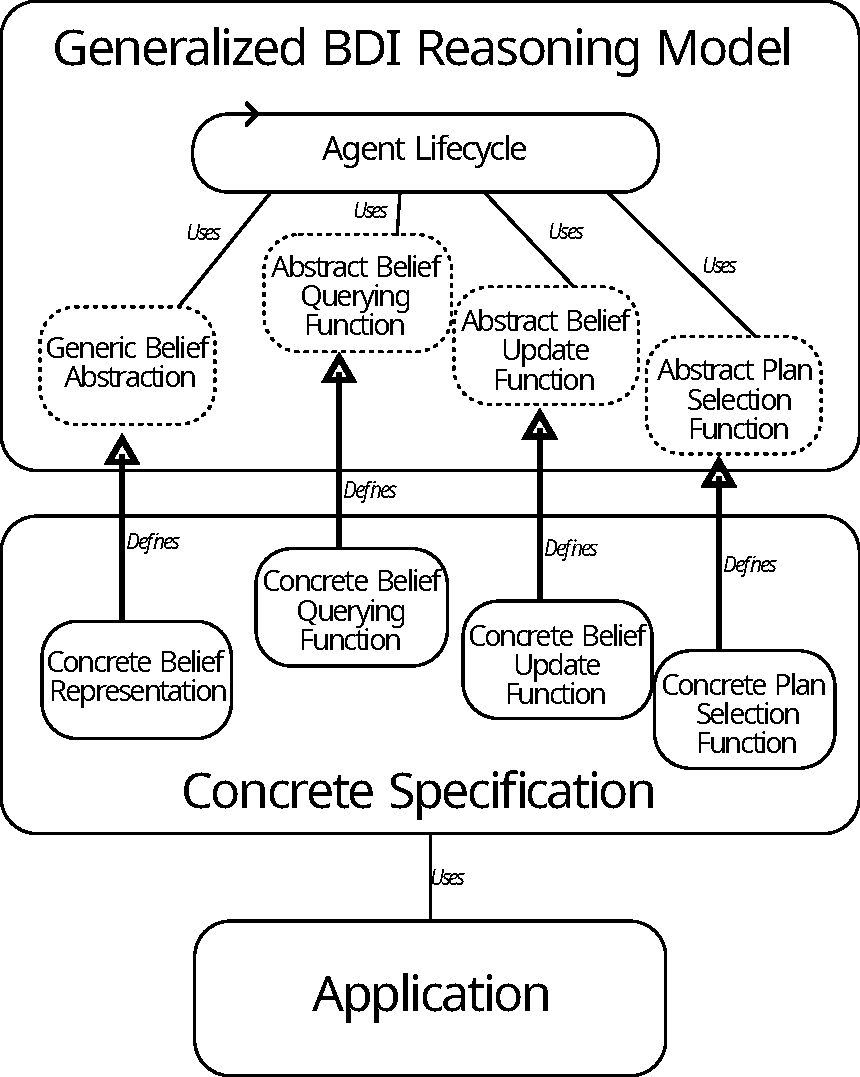
\includegraphics[width=0.5\linewidth]{figures/hyperagents25/architecture}
\end{figure}

However,
separating the reasoning cycle of \ac{BDI} agents from knowledge representation is complex,
as the two are deeply intertwined~\cite{DBLP:conf/dalt/MoreiraVBH05}.
%
Consider for instance these fundamental operations:
%
\begin{inlinelist}
  \item \emph{plan selection}
  % is the process of selecting a plan to achieve a goal among the ones available,
  % which evaluation of applicability is strictly related on how beliefs are represented in the belief base;
  depending on conditions to be tested against the belief base;

  \item \emph{belief querying}
  % is the process of retrieving information from the belief base;
  as part of a plan, for the sake of decision-making;

  \item \emph{belief update}
  % is the process of updating the belief base with new information.
  for the sake of updating the agent's knowledge,
  as part of a course of action.
\end{inlinelist}
%
In \ac{LP}-based frameworks,
these would simply rely on logic unification and resolution,
whereas in a generalised \ac{BDI} engine,
each operation may rely on different matching strategies.
%
For instance,
for Semantic Hypermedia agent,
one may rely on \ac{RDF} and \ac{OWL} for beliefs representation,
\acs{SPARQL} for belief querying and update,
and \ac{SWRL} for plan selection and ontological inference%
%
% In the latter case,
% agent developers would be able to plug-in convenient syntaxes and ad-hoc technologies,
% hence customising how the generic \ac{BDI} engine operates upon beliefs in all such cases,
---thus addressing \ref{req:reasoning} and \ref{req:query}.

% The integration of \ac{BDI} \ac{MAS} with heterogeneous syntax representations
% can be performed with a layered architecture of the framework.
% %
% The layered architecture proposed is composed of:
The generalised \ac{BDI} engine can be realised with a layered architecture (see \Cref{fig:generalised-bdi-architecture}) comprising three layers.
%
\begin{enumerate*}[label={\emph{Layer \arabic*}:}]
  \item \textbf{generalised \ac{BDI} reasoning layer},
  where the agent's deliberation process is implemented as a reasoning cycle,
  yet agnostic to how beliefs are represented and manipulated.
  %
  This is where
  agents' intentions are maintained
  and updated as agents perceive,
  decide what to do,
  and finally act.
  %
  Any operation involving belief bases should rely on some \emph{abstract} \acs{API},
  to be implemented by the next layer.
  %
  \item \textbf{concrete specification layer},
  where the aforementioned \acs{API} is implemented to provide concrete operations on the belief base.
  %
  This layer acts as an adapter between the generalised \ac{BDI} reasoner
  and the specific knowledge representation technologies of choice.
  %
  Lastly,
    \item \textbf{application layer},
  where actual goals, plans, and interactions of a \ac{MAS} are defined
  to tackle some specific use case.
\end{enumerate*}

% The main advantages of this isolation are: reuse of the same reasoning engine across multiple domains, and Better support for semantic web standards and open-world reasoning.

Requirement \ref{req:actions} although not directly addressed by the approach,
could be integrated with the techniques already being explored in the \ac{hMAS} community (cf. \Cref{sec:related-works}), benefitting from the possibility of choosing the most suitable knowledge representation technology
to facilitate their agents to discover new actions at runtime in the hypermedia environment.

%==========================================================
\section{Conclusion}
\label{sec:conclusion}
%==========================================================

In this chapter, 
we present a gap analysis between \ac{BDI} agents and semantic hypermedia,
showing how they are difficult to integrate due to the different technologies and paradigms they rely on.
%
We identify a set of ideal requirements, finding that none of the surveyed related works fully satisfy them
and propose to implement them through a generalised \ac{BDI} engine that can be tailored to use \ac{RDF} and \ac{OWL} as knowledge representation technologies.

Future work will focus on implementing the architecture proposed in \Cref{sec:generalised-bdi-engine}
and explore how to support \ac{hMAS} developers with syntax extensions
and tools to ease the development of \ac{BDI} agents in hypermedia environments
within our \ac{BDI} programming framework \jakta{}~\cite{DBLP:journals/sncs/BaiardiBCP24}.
